\chapter{Genetic Drift and Neutral Diversity}

Various sources of randomness are inherent in evolution.  One major source of
stochasticity in population genetics is genetic drift.  Genetic drift occurs
because more or less copies of an allele by chance can be transmitted to the
next generation. This can occur because by chance the individuals carrying a
particular allele can leave more or less offspring in the next generation. In a
sexual population genetic drift also occurs because Mendelian transmission
means that only one of the two alleles in an individual, chosen at random at a
locus, is transmitted to the offspring. 

Genetic drift can play a role in the dynamics of all alleles and populations,
but it will play the biggest role for neutral alleles. A neutral polymorphism
occurs when the segregating alleles at a polymorphic site have no discernible
differences in their effect on fitness. We'll make clear what we mean by discernible later, for
the moment think of this as ``no effect" on fitness. 


\subsection{Loss of heterozygosity due to drift.} \label{LossofHet} 

Genetic drift will, in the absence of new mutations, slowly purge our
population of neutral genetic diversity as alleles slowly drift to high or low
frequencies and are lost or fixed over time. \\

Imagine a population of a constant size $N$ diploid individuals, and that we
are examining a locus segregating for two alleles that are neutral with respect
to each other.  This population is randomly mating with respect to the alleles
at this locus. See Figures \ref{fig:LossHet_two_alleles} and
\ref{fig:LossHet_many_alleles} to see how genetic drift proceeds, by tracking
alleles within a small population. \\

In generation $t$ our current level of heterozygosity is $H_t$,
i.e. the probability that two randomly sampled alleles in generation
$t$ are non-identical is $H_t$. Assuming that the mutation rate is
zero (or vanishing small), what is our level of heterozygosity in
generation $t+1$?\\

\begin{figure}
\begin{center}
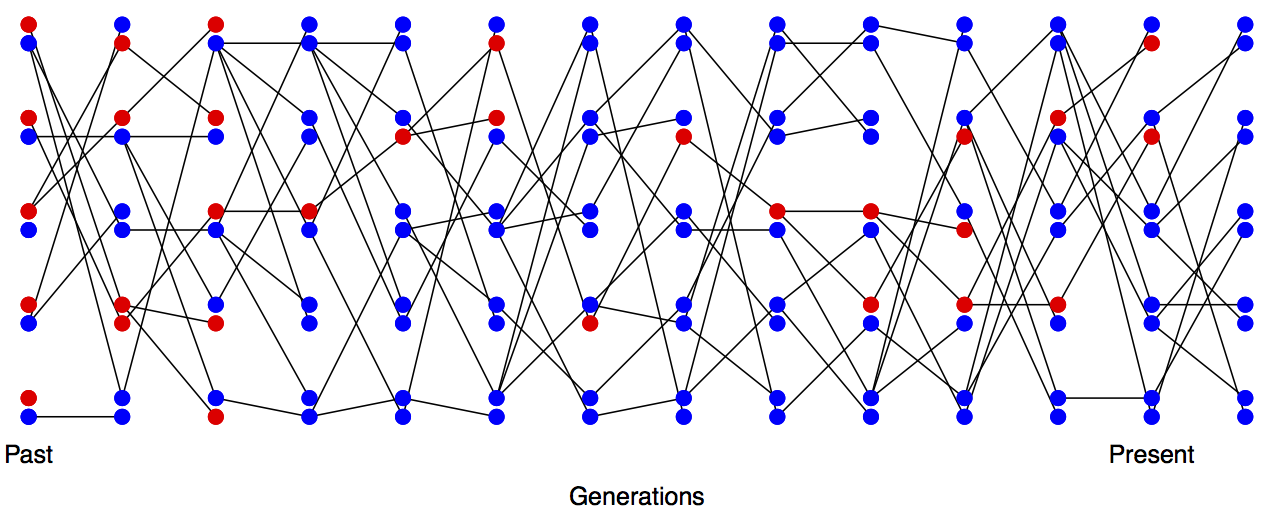
\includegraphics[width= \textwidth]{figures/Loss_of_he_col_two_alleles.png}
\end{center}
\caption{Loss of heterozygosity over time, in the absence of new
  mutations. A diploid population of 5 individuals over the
  generations, with lines showing transmission. In the first
  generation every individual is a heterozygote.} \label{fig:LossHet_two_alleles}
\end{figure} 

\begin{figure}
\begin{center}
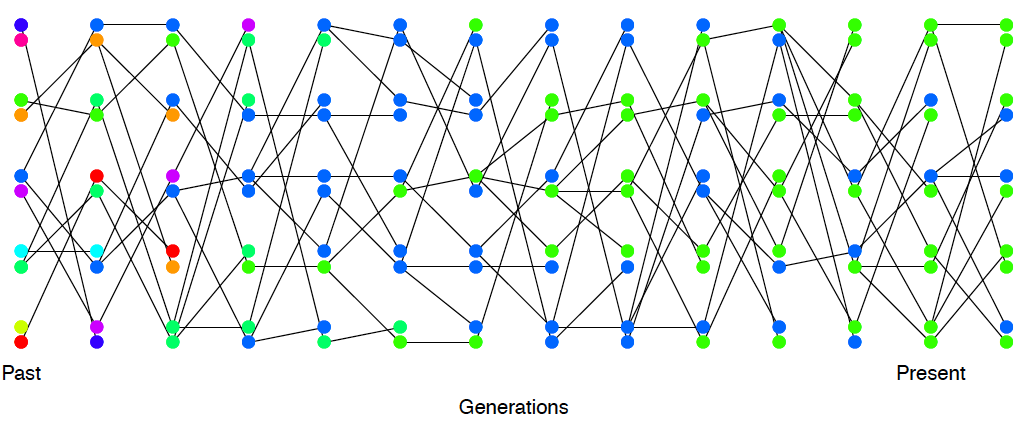
\includegraphics[width= \textwidth]{figures/Loss_of_het_2_many_alleles.png}
\end{center}
\caption{Loss of heterozygosity over time, in the absence of new
  mutations. A diploid population of 5 individuals. In the first generation I colour every allele a different
colour so we can track their descendants.} \label{fig:LossHet_many_alleles}
\end{figure} 

In the next generation ($t+1$) we are looking at the alleles in the
offspring of generation $t$. If we randomly sample two alleles in generation
$t+1$ which had different parental alleles in generation $t$ then it
is just like drawing two random alleles from generation $t$. So the
probability that these two alleles in generation $t+1$, that have
different parental alleles in generation $t$, are non-identical is
$H_t$. \\

Conversely, if our pair of alleles have the same parental allele in
the proceeding generation (i.e. the alleles are identical by descent
one generation back) then these two alleles must be identical (as we
are not allowing for any mutation). \\

\marginnote{
\begin{question} You are in charge of maintaining a population of delta smelt in the Sacramento river delta. Using a large set of microsatellites you
  estimate that the mean level of heterozygosity in this population is 0.005.
  You set yourself a goal of maintaining a level of heterozygosity of at least
  0.0049 for the next two hundred years. Assuming that the smelt have a
  generation time of 3 years, and that only genetic drift affects these loci.
  What is the smallest fully outbreeding population that you would need to
maintain to meet this goal?  
\end{question}
}

In a diploid population of size $N$ individuals there are $2N$ alleles. The
probability that our two alleles have the same parental allele in the
proceeding generation is $\nicefrac{1}{(2N)}$, the probability that they have
different parental alleles is is $1-\nicefrac{1}{(2N)}$. So by the above
argument the expected heterozygosity in generation $t+1$ is
%
\begin{equation}
H_{t+1} = \frac{1}{2N} \times 0 + \left(1-\frac{1}{2N} \right)H_t
\end{equation}
%
By this argument if the heterozygosity in generation $0$ is $H_0$ our
expected heterozygosity in generation $t$ is
%
\begin{equation}
H_t = \left(1-\frac{1}{2N} \right)^tH_0
\end{equation}
%
i.e. the expected heterozygosity with our population is decaying
geometrically with each passing generation. If we assume that $\nicefrac{1}{(2N)}
\ll 1$ then we can approximate this geometric decay by an exponential
decay (see Question \ref{geo_question} below), such that
%
\begin{equation}
H_t =H_0 \exp \left(-\frac{t}{2N} \right)  
\end{equation}
%
i.e. heterozygosity decays exponentially at a rate
$\nicefrac{1}{(2N)}$.

Note how this picture of decreasing heterozygosity is in contrast to the
consistency of Hardy--Weinberg equilibrium of the previous chapter. 
However, our Hardy-Weinberg \emph{proportions} hold in forming each new
generation. As the offspring genotypes in the next generation ($t+1$) represent a random
draw from the previous generation ($t$). If the parental frequency is $p_t$ we
\emph{expect} a proportion $2p_t(1-p_t)$ of our offspring to be
heterozygotes (and HW proportions for our homozygotes). However, because of population size is finite the
observed genotype frequencies in the offspring will (likely) not match exactly with our
expectations. As our genotype frequencies likely change slightly due
to sampling, biologically this reflects random variation in family size
and Mendelian segregation, the allele frequency will changed. 
Therefore, while each generation represents a sample from
Hardy-Weinberg proportions based on the generation before, our
genotype proportions is not a equilbrium (an unchanging state) as the
underyling allele frequency changes over the generations. We'll develop some mathematical models for these allele
frequency changes later on. For now we'll simply note that
under our simple model of drift (formally the Wright Fisher model) our
allele count in the $t+1^{th}$ generation represents a binomial sample
(of size $2N$) from the population frequency $p_t$ in the previous
generation.  

% generation $t$ may differ
%from that of $t+1$. We'll develop some mathematical models for these allele
%frequency changes 
 %from the previous generation we are
%drawing alleles at random from the  
%Here, the
%freqeuncy of each genotype will likely change, due to chance fluctuations in
%the underlying allele frequency $p$. While within a single generation
%Hardy--Weinberg proportions are maintained (at least approximately), across
%generations the genotypic frequencies change with allele frequency. The change
%in allele frequencies is due to drift: due to random variation in family size
%and Mendelian segregation, the allele frequency in generation $t$ may differ
%from that of $t+1$. We'll develop some mathematical models for these allele
%frequency changes later on.


\begin{marginfigure}
\begin{center}
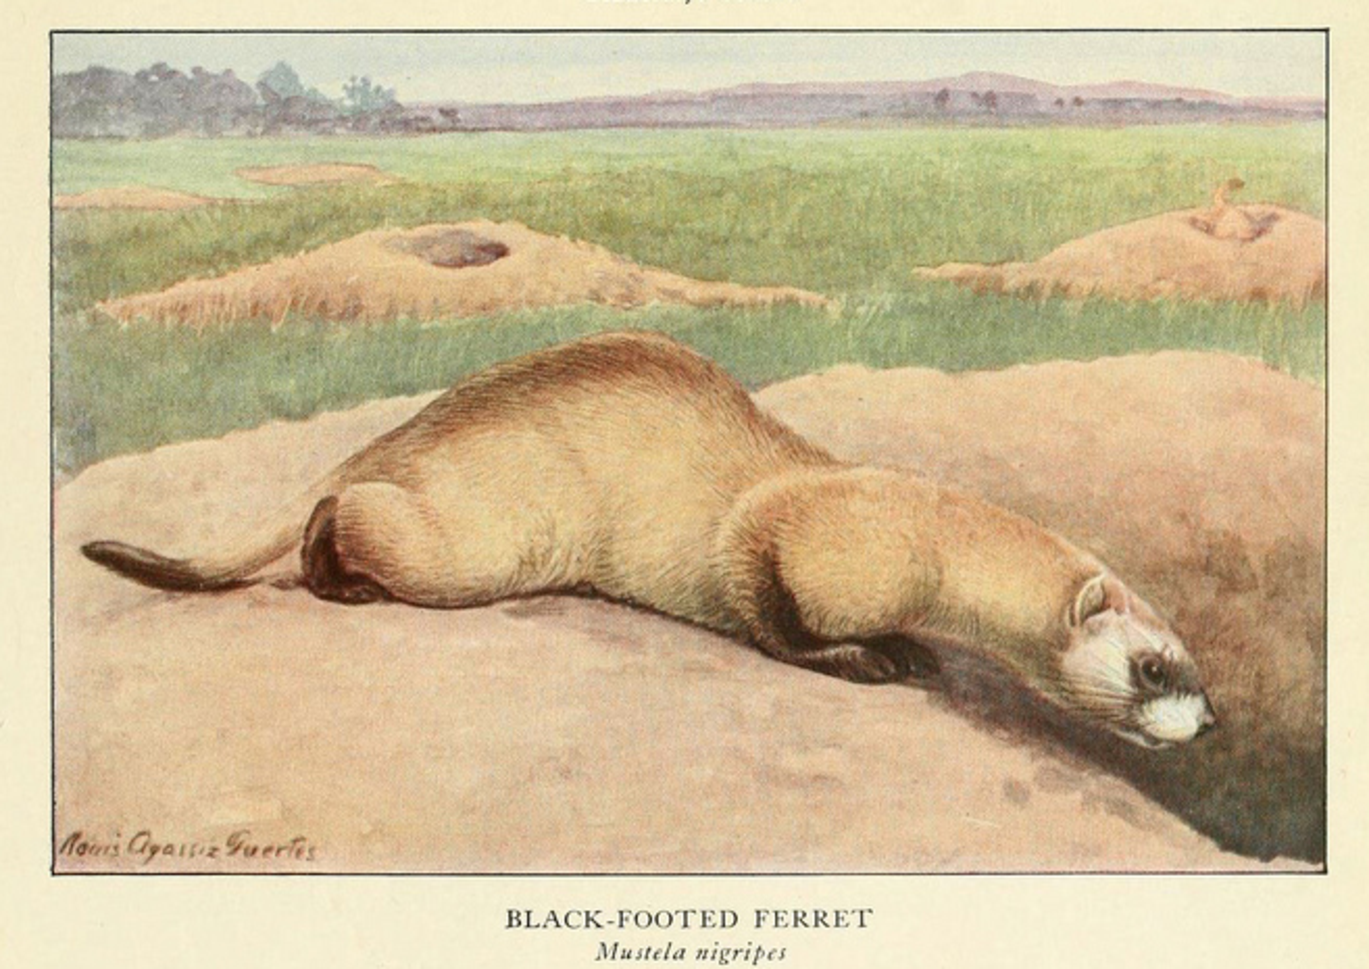
\includegraphics[width=\textwidth]{illustration_images/Genetic_drift/Black_footed_ferrets/Black_footed_ferret.pdf}
\end{center}
\caption{The black-footed ferret ({\it M. nigripes}). Wild animals of North America, The National geographical
  society, 1918. BHL} \label{fig:black_footed_ferret}  
\end{marginfigure} 

\begin{marginfigure}
\begin{center}
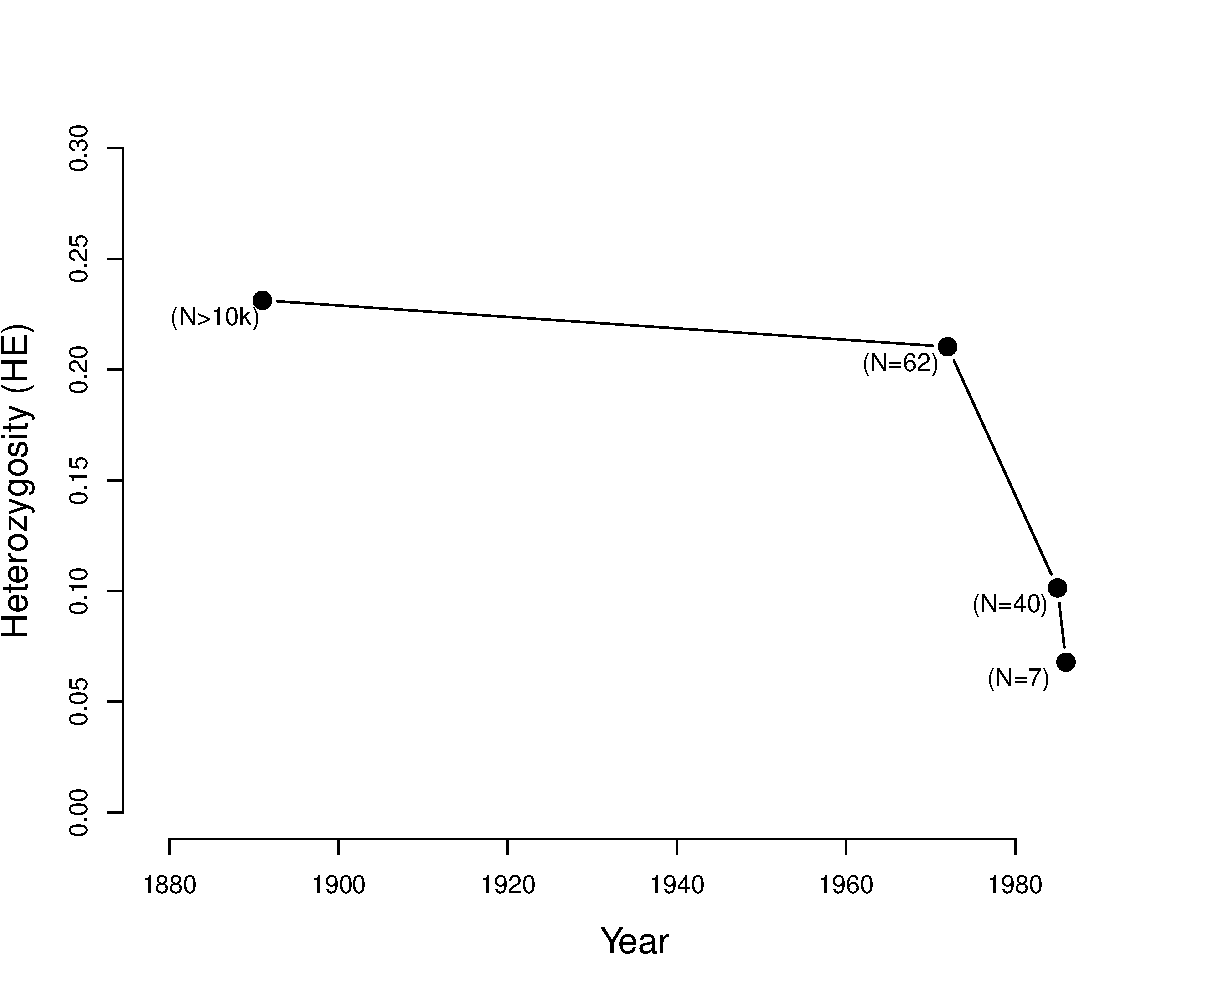
\includegraphics[width= \textwidth]{Journal_figs/genetic_drift/black_footed_ferrets/black_footed_ferrets_He.pdf}
\end{center}
\caption{Loss of heterozygosity in the Black-footed Ferrets. Redrawn
  from \citeauthor{Wisely:02}.} \label{fig:LossHet_ferrets}  
\end{marginfigure} 

To see how a decline in population size can affect levels of
heterozygosity lets consider the case of black-footed ferrets ({\it Mustela
  nigripes}). The black-footed ferrets population size of the declined dramatically through the twentifth century due
to destruction of their habitat.  In 1979 what was thought to
be the the last ferret died in captivity, and they thought to be
extinct. In 1981 a very small, wild population were rediscovered ($40$ individuals), but in 1985 this
suffered a number of disease outbreaks. All of the $18$ remaining wild individuals
were brought into captivity, 7 of these individuals
reproduced. \citeauthor{Wisely:02} measured heterozygosity at a number
of microsatellites in indviduals from museum collections, see Figure \ref{fig:LossHet_ferrets}.
Thanks to intense captive breeding efforts and conservation work a
wild population of over 300 individuals has be established
since. However, because all of these individuals are descended from
those 7 individuals who survived the bottleneck diversity levels
remain low. 


\begin{question} \label{geo_question} In mathematical population genetics, a
  commonly used approximation $(1-x) \approx e^{-x}$ for $x << 1$ (formally
  this follows from the Taylor series expansion of $\exp(-x)$ ignoring second
  order terms of $x$).  This is especially useful for approximating a geometric
  decay process by an exponential decay process, e.g. $(1 - x)^t \approx
  e^{-xt}$. Using R, check how good of an approximation this is for three
  values of x, $x = 0.5, 0.1, 0.01$. Do this by plotting the geometric decay as
  points, and the exponential decay as a curve, using different colors for each
  of these three values. Note that you should have a discrete timescale for the
  geometric decay (e.g. using \texttt{t=seq(0, 18)}) and a near continuous scale
  for the exponential decay (e.g. using \texttt{t=seq(0, 18, length.out=100)}.
  Print off your graph and hand it in. 
    % max <- 18; x <- seq(0, max); x1 <- seq(0, max, length.out=100); plot(x, (1-0.5)^x, col='purple', pch=19); lines(x1, exp(-0.5*x1), col='purple'); points(x, (1-0.1)^x, pch=19, col='orange'); lines(x1, exp(-0.1*x1), col='orange'); points(x, (1-0.01)^x, pch=19, col='green'); lines(x1, exp(-0.01*x1), col='green') # messy but works

\end{question}

\subsection{Levels of diversity maintained by a balance between
 mutation and drift} \label{DriftMutationBalance}
\graham{Move this to a supp? And just have $\pi$}
Looking backwards in time from one generation to the next, we are going to say
that two alleles which have the same parental allele (i.e. find their common
ancestor) in the preceding generation have \emph{coalesced}, and refer to this
event as a \emph{coalescent event}.

The probability that our pair of randomly sampled alleles have coalesced in the
preceding generation is $\nicefrac{1}{(2N)}$, the probability that our pair of
alleles fail to coalesce is $1-\nicefrac{1}{(2N)}$. 

The probability that a mutation changes the identity of the
transmitted allele is $\mu$ per generation. So the probability of no
mutation occurring is $(1-\mu)$. We'll assume that when a mutation
occurs it creates some new allelic type which is not present in the
population. This assumption (commonly called the infinitely-many-alleles model) makes the math slightly cleaner, and also
is not too bad an assumption biologically. See Figure
\ref{fig:Mut_Sel_balance} for a depiction of mutation-drift balance in
this model over the generations.

This model let's us calculate when our two alleles last shared a common
ancestor and whether these alleles are identical as a result of
failing to mutate since this shared ancestor.  For example we can work out the probability that our
two randomly sampled alleles coalesced $2$ generations in the past
(i.e. they fail to coalesce in generation $1$ and then coalescent in
generation $2$), and
that they are identical as
\begin{equation}
\left(1- \frac{1}{2N} \right) \frac{1}{2N} (1-\mu)^4
\end{equation}
note the power of $4$ is because our two alleles have to have failed
to mutate through $2$ meioses each. 

More generally the probability that our alleles coalesce in generation
$t+1$ and are identical due to no mutation to either allele in the
subsequent generations is
%
\begin{equation}
P(\textrm{coal. in t+1 \& no mutations}) =  \frac{1}{2N} \left(1- \frac{1}{2N} \right)^t \left(1-\mu \right)^{2(t+1)}
\end{equation}
%
to make this slightly easier on ourselves let's further assume that $t
\approx t+1$ and so rewrite this as:
\begin{equation}
P(\textrm{coal. in t+1 \& no mutations}) \approx \frac{1}{2N} \left(1- \frac{1}{2N} \right)^t \left(1-\mu \right)^{2t}
\end{equation}
%

This gives us the approximate probability that two alleles will coalesce in the
$(t+1)^\text{th}$ generation. In general, we may not know when two alleles may
coalesce: they could coalesce in generation $t=1, t=2, \ldots $, and so on.
Thus, to calculate the probability that two alleles coalesce in \emph{any}
generation before mutating, we can write:

\begin{align*}
  P(\textrm{coal. in any generation \& no mutations}) \approx & P(\textrm{coal. in} \; t=1 \; \textrm{\& no mutations}) \; + \\ 
&  P(\textrm{coal. in} \; t=2 \; \textrm{\& no mutations}) + \ldots \\
  %P(\textrm{coal. in} \; t=3 \; \textrm{\& no mutations})  +\ldots \\
  = & \sum_{t=1}^\infty P(\textrm{coal. in } \; t \; \textrm{generations \& no mutation})
\end{align*}
%
which follows from the fact that coalescing in a particular generation is
mutually exclusive with coalescing in a different generation and basic probability.

While we could calculate a value for this sum given $N$ and $\mu$, it's
difficult to get a sense of what's going on with such a complicated expression.
Here, we turn to a common approximation in population genetics (and all applied
mathematics), where we assume that $\nicefrac{1}{(2N)} \ll 1$ and $\mu \ll 1$.
This allows us to approximate the geometric decay as an exponential decay.
Then, the probability two alleles coalesce in generation $t+1$ and don't mutate
can be written as:
%
\begin{align} P(\textrm{coal. in t+1 \& no mutations}) &\approx \frac{1}{2N}
\left(1- \frac{1}{2N} \right)^t \left(1-\mu \right)^{2t} \\ 
& \approx \frac{1}{2N} e^{-t/(2N)} e^{-2\mu t } \\
&=\frac{1}{2N} e^{-t(2\mu+1/(2N))} \end{align} 
%
and then we simply approximate the summation by an integral, giving us:
%
\begin{figure} \begin{center} 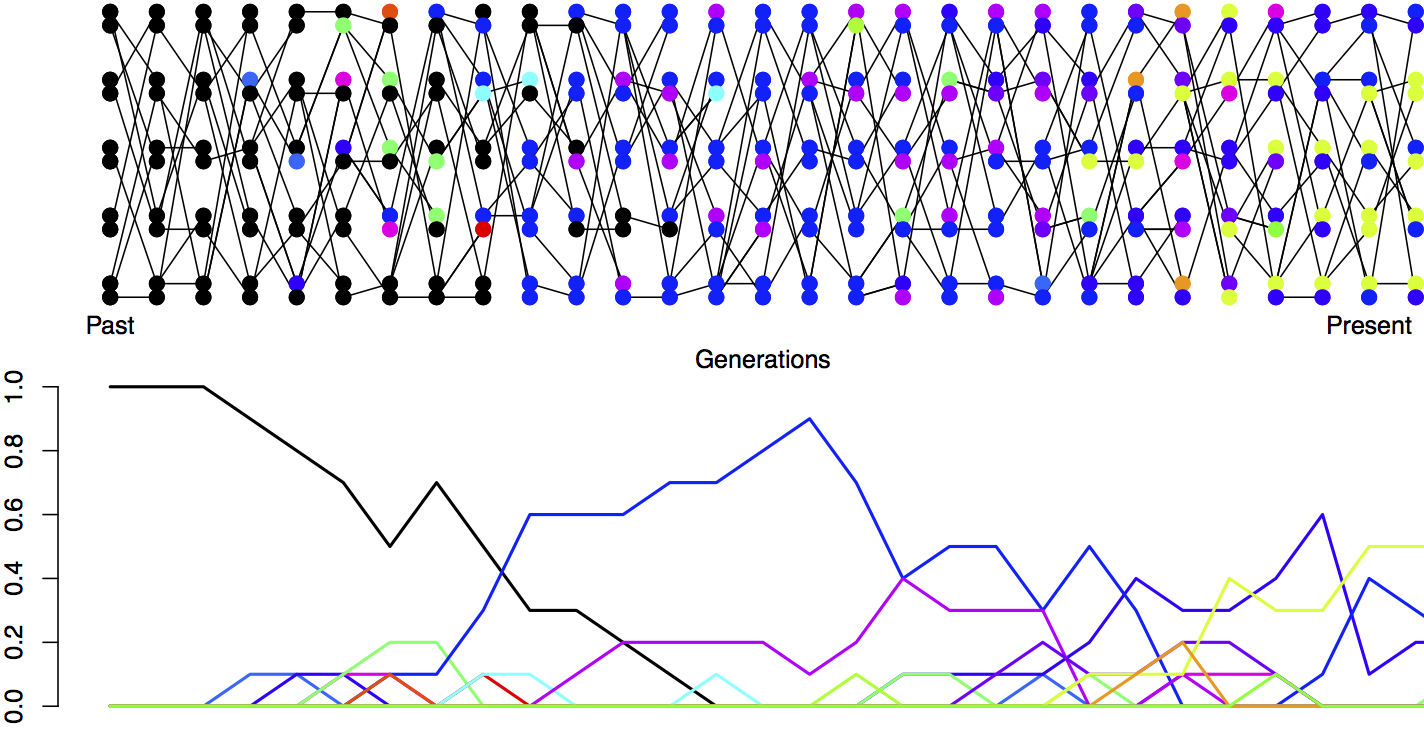
\includegraphics[width= 0.8
\textwidth]{figures/Mut_drift_balance.png} \end{center} \caption{Mutation-drift
balance. A diploid population of 5 individuals. In the first generation
everyone has the same allele (black). Each generation the transmitted allele
can mutate and we generate a new colour. In the bottom plot I trace the
frequency of alleles in our population over time.} \label{fig:Mut_Sel_balance}
\end{figure} 

\begin{equation}
\frac{1}{2N} \int_0^{\infty} e^{-t(2\mu+1/(2N))} dt =
\frac{1/(2N)}{1/(2N)+2\mu} = \frac{1}{1+4N\mu}
\end{equation}

Doing so gives us the probability that our two alleles coalesce at some point
in time, and do not mutate on either ancestral lineage to their common
ancestor. Equivalently, this can be thought about as the probability our two
alleles coalesce \emph{before} mutating. 

Then, the complementary probability that our pair of alleles are non-identical
(or heterozygous) is simply one minus this. This gives the equilibrium
heterozygosity in a population at equilibrium between mutation and drift:

\begin{equation}
  H = \frac{4N\mu}{1+4N\mu} \label{eqn:hetero}
\end{equation}
This compound parameter $4N\mu$, the population-scaled mutation rate,
will come up a number of times so we'll give it its own name
\begin{equation}
\theta = 4N\mu
\end{equation}

So all else being equal, species with larger population sizes should
have proportionally higher levels of neutral polymorphism.  If you've read to here please email Prof Coop a picture of JBS Haldane
in a striped suit with the title ``I'm reading the chapter 2 notes''. (It's well worth googling JBS Haldane and read more about his life,
he's a true character and one of the last great polymaths. )

\subsection{The effective population size}
\marginnote{the effective population size ($N_e$) is the population size that
would result in the same rate of drift in an idealized constant population size
as that observed in our true population (following our modeling
assumptions).}

In practice populations rarely conform to our assumptions of being
constant in size with low variance in reproduction success. Real
populations experience dramatic fluctuations in size, and there is
often high variance in reproductive success. Thus rates of drift in
natural populations are often a lot higher than the census population
size would imply. See Figure \ref{fig:LossHet_varying_pop}  for a depiction of
a repeatedly bottlenecked population losing diversity at a fast rate.

\begin{figure}
\begin{center}
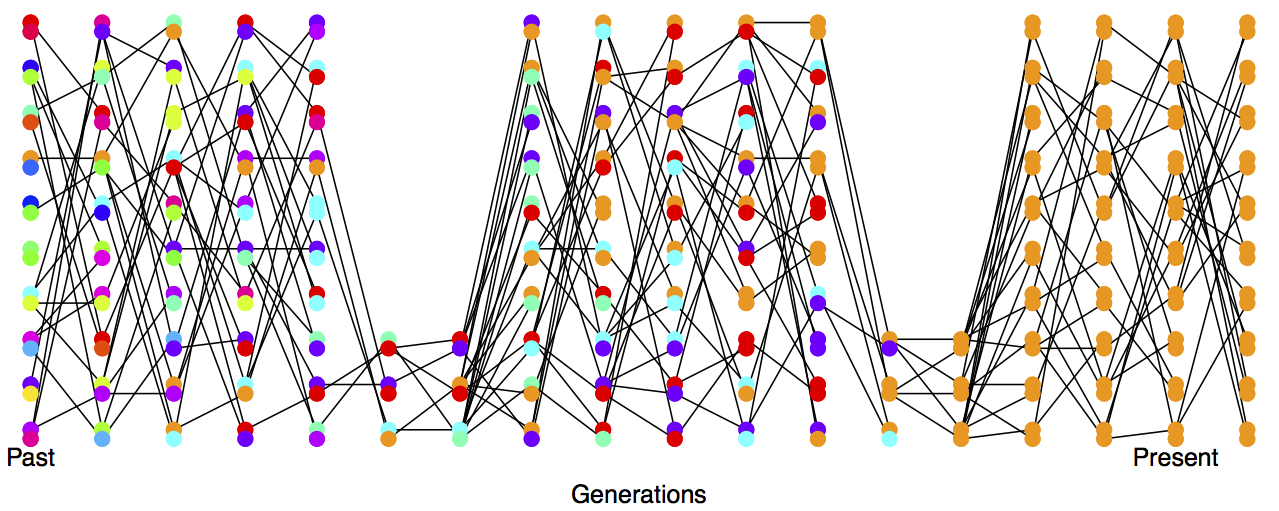
\includegraphics[width= \textwidth]{figures/Loss_of_he_col_alleles_varying_pop_dark.png}
\end{center}
\caption{Loss of heterozygosity over time in a bottlenecking population. A diploid population of 10 individuals, that bottlenecks
  down to three individuals repeatedly. In the first generation I colour every allele a different
colour so we can track their descendants, there are no new
  mutations.} \label{fig:LossHet_varying_pop}  
\end{figure} 


To cope with this population geneticists often invoke the concept of
an \emph{effective population size} ($N_e$). In many situations (but not all), departures from model assumptions can be captured by substituting $N_e$ for $N$.
\\

\marginnote{
To see this note that if $1/(N_i)$ is
small, then we can approximate \eqref{eqn:var_pop_coal} by 
\begin{equation}
\prod_{i=1}^{t} \exp \left( -\frac{1}{2N_i} \right)   =
\exp \left(- \sum_{i=1}^{t} \frac{1}{2N_i} \right) .
\end{equation}
This is same form but
the exponent has changed. Comparing the exponent in the two cases we see
\begin{equation}
\frac{t}{2N} = \sum_{i=1}^{t} \frac{1}{2N_i} 
\end{equation}
so that if we want a constant effective population size ($N_e$) that has the same
rate of loss of heterozygosity as our variable population we need to set
$N=N_e$ and rearrange this to give \eqref{eq:Ne_harmonic}.} 

If population sizes vary rapidly in size, we can (if certain conditions are met)
replace our population size by the harmonic mean population size.
Consider a diploid population of variable size, whose size is $N_t$ $t$ generations into the
past. The probability our pairs of alleles have not coalesced by the generation $t^{th}$ is
given by
\begin{equation}
\prod_{i=1}^{t} \left(1-\frac{1}{2N_t} \right) \label{eqn:var_pop_coal}
\end{equation}
note that this is simply collapses to our original expression
$\left(1-\frac{1}{2N } \right)^t $ if $N_i$ is constant. 

The rate of loss of heterzygosity in this population is equivalent to
a population of effective size
\begin{equation}
N_e =\frac{1}{\frac{1}{t} \sum_{i=1}^{t} \frac{1}{N_i} }. \label{eq:Ne_harmonic}
\end{equation}
this is the harmonic mean of the varying population size.


Thus our
effective population size, the size of an idealized constant
population which matches the rate of genetic drift, is the harmonic
mean true population size over time. The harmonic mean is very
strongly affected by small values, such that if our population size is
one million $99\%$ of the time but drops to a $1000$ every hundred or
so generations, $N_e$ will be much closer to $1000$ than a
million. \\


%would result in the same rate of drift
%Luckily, in many (not all) situations, departures from model assumptions can be captured by substituting Ne for N, i.e., by plugging in a fictitious N that leads to the same level of genetic drift as observed.



Variance in reproductive success will also affect our effective
population size. Even if our population has a large constant size of $N$
individuals, if only small proportion of them get to reproduce then
the rate of drift will reflect this much small number of reproducing
individuals. See Figure \ref{fig:LossHet_varying_RS} for a depiction of the higher rate of drift
in a population where there is high variance in reproductive success.

\marginnote{When our two alleles pick an ancestor, $25\%$ of the time
our alleles were both in a female ancestor in which case they coalesce
with probability $1/(2N_F)$, and $25\%$ of the time they are both in a
male ancestor in which case they coalesce with probability
$1/(2N_M)$. The remaining $50\%$ of the time our ancestral lineages
are in two individuals are different sexes in a generation so cannot
coalescence.  Therefore, our probability of coalescence in the preceding
generation is
\begin{equation}
\frac{1}{4}\frac{1}{2N_M}+\frac{1}{4}\frac{1}{2N_F} %=
%\frac{1}{8}\frac{N_F+N_M}{N_FN_M} 
\end{equation}
i.e. the rate of coalescence is the harmonic mean of the two
sexes population sizes, 
equating this to $\frac{1}{2N_e}$}

\begin{marginfigure}
\begin{center}
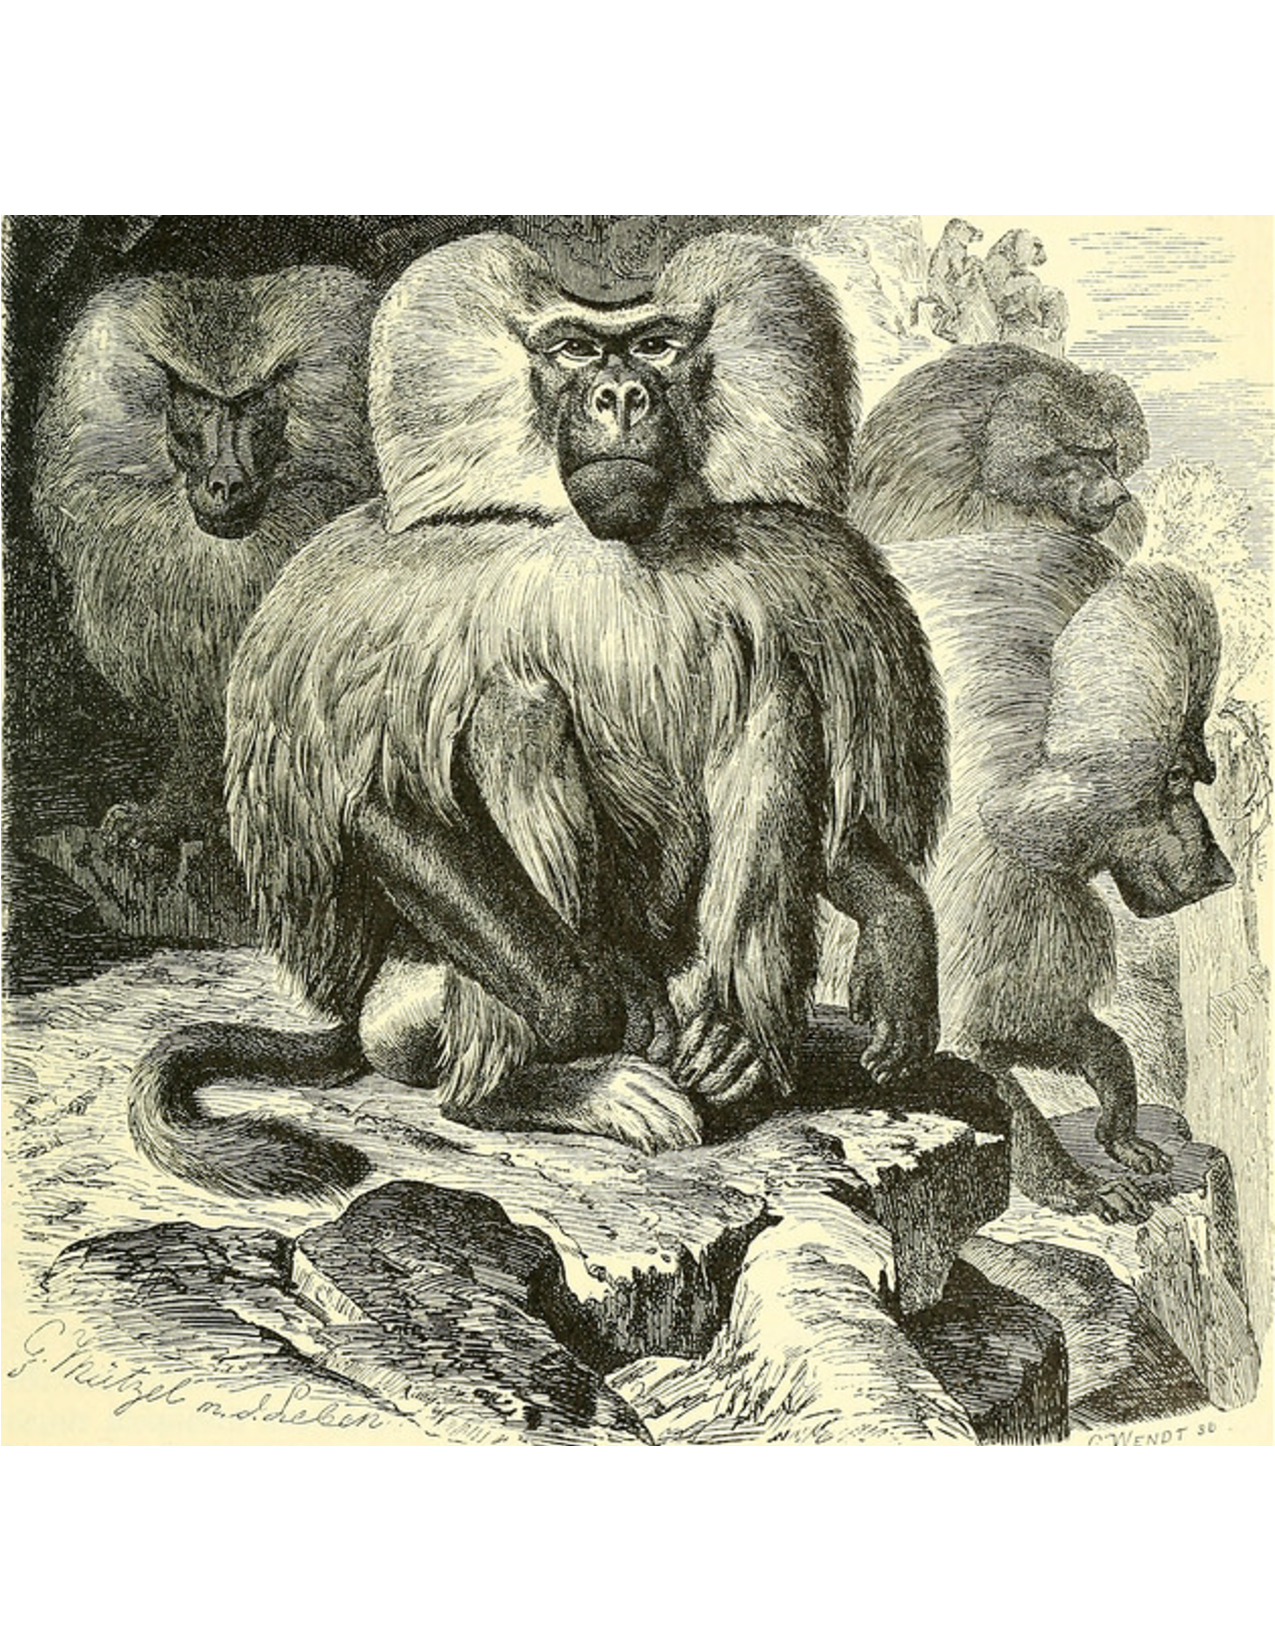
\includegraphics[width= 0.7 \textwidth]{illustration_images/Genetic_drift/Hamadryas_baboon/Hamadryas_baboon.pdf}
\end{center}
\caption{Male Hamadryas baboons. Brehm's Tierleben. Brehm,
  A.E. 1893. Up to ten females live in a harem with a single male.  %Brehm's animal life
} \label{fig:Hamadryas_baboon}  
\end{marginfigure} 

While every individual has a mother an a father, not every individual
gets to be a parent. In practice in many populations far more females
get to reproduce than males. If only $N_M$ males get to contribute to the next
generation and $N_F$ females get to contribute to the next
generation, we find
\begin{equation}
N_e = \frac{4N_FN_M}{N_F+N_M}
\end{equation}
Thus if reproductive success is very skewed in one sex (e.g. $N_M \ll
N/2$) our effective population size will be much reduced as a result.\\

\begin{question}
You are studying a population of 1000 Hamadryas baboons. Assuming a
1/10 male to female sex ratio of matings. What is the effective
population size?
 \end{question}

\begin{figure}
\begin{center}
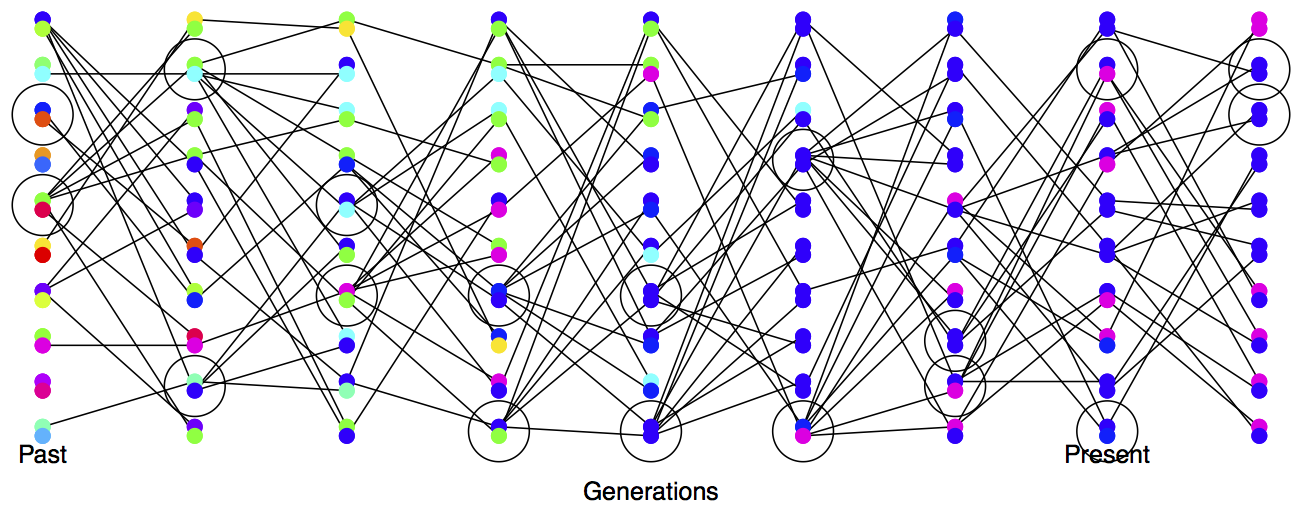
\includegraphics[width= \textwidth]{figures/Loss_of_he_col_alleles_varying_RS.png}
\end{center}
\caption{High variance on reproductive success increases the rate of genetic drift. A diploid population of 10 individuals, where the circled
  individuals have much higher reproductive success. In the first generation I colour every allele a different
colour so we can track their descendants, there are no new
  mutations.} \label{fig:LossHet_varying_RS}
\end{figure} 


\section{The Coalescent and patterns of neutral diversity}

\begin{quote}
"Life can only be understood backwards; but it must be lived
forwards." -- Kierkegaard
\end{quote}

\paragraph{Pairwise Coalescent time distribution and the number of
 pairwise differences.}
Thinking back to our calculations we made about the loss of neutral heterozygosity
and equilibrium levels of diversity (in Sections \ref{LossofHet} and \ref{DriftMutationBalance}), you'll note that we could first specify
what generation a pair of sequences coalesce in, and then calculate
some properties of heterozygosity based on that. That's because neutral
mutations do not affect the probability that an individual transmits
that allele, so don't affect the way in which we can trace ancestral lineages
back. \\


As such it will often be helpful to consider the time to the common
ancestor of a pair of sequences, and then think of the impact of that
on patterns of diversity. See Figure \ref{fig:Coalescent_simulation}
for an example of this. 

\begin{figure}
\begin{center}
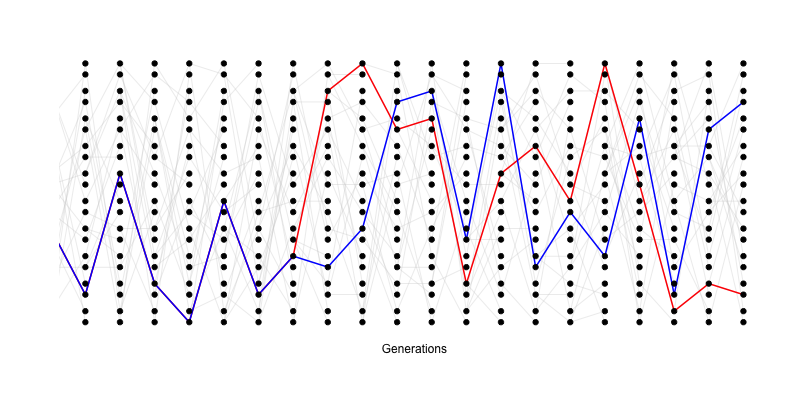
\includegraphics[width=\textwidth]{figures/Coalescent.png}
\end{center}
\caption{A simple simulation of the coalescent process. The simulation
  consists of a diploid population of 10 individuals (20 alleles). In
  each generation, each individual is equally likely to be the parent
  of an offspring (and the allele transmitted is indicated by a light
  grey line).  We track a
  pair of alleles, chosen in the present day, back 14 generations
  untill they find a common ancestor.} \label{fig:Coalescent_simulation}
\end{figure}

\marginnote{Blurring our eyes a little we can see  that \ref{eqn:coal_time_dist} is
\begin{equation}
\approx \frac{1}{2N} e^{-t/(2N)} 
\end{equation}
thus if we wanted a continuous random variable we could say that the coalescent time of a pair of sequences ($T_2$) is
approximately exponentially distributed with a rate $1/(2N)$, i.e. $T_2 \sim \text{Exp}\left( 1/(2N) \right)$. }

\graham{fix equation numbers here}
The probability that a pair of alleles
have failed to coalesce in $t$ generations and then coalesce in the
$t+1$ generation back is
\begin{equation}
  \frac{1}{2N} \left(1- \frac{1}{2N} \right)^{t} \label{eqn:coal_time_dist}
\end{equation}
Thus the coalescent time of our pair of alleles is a Geometrically distributed random variable,
where the probability of success is $1/(2N)$, we've denote this by $T_2 \sim  \text{Geo}(1/(2N))$
The mean coalescent time of a pair of a pair of alleles is $2N$ generations\\

Conditional on a pair of alleles coalescing $t$ generations ago
there are $2t$ generations in which a mutation could occur. If the per
generation mutation rate is $\mu$ then the expected number of
mutations between a pair of alleles coalescing $t$ generations ago is
$2 t\mu$

As our expected coalescent time is $2N$ generations (which follows from the expected value of exponential distributions), the expected
number of mutations separating two alleles drawn at random from the
population is
%
\begin{align}
  \E(j) &= 2\mu\E(t) \\ \nonumber
  &= 4N\mu \\
  &= \theta \nonumber
\end{align}
We'll assume that mutations never happen at the same site twice,
i.e. no multiple hits, such that we get to see all of the mutation events that separate our pair
of sequences \sidenote{This is called the infinitely-many-sites assumption,
which should be fine if $N\mu_{BP} \ll 1$, where $\mu_{BP}$ is the mutation rate per base pair).} Thus the number of
mutations between a pair of sites is the observed number of
differences between a pair of sequences. \\

We'll denote the observed number of pairwise differences at putatively neutral
sites separating a pair of sequences as $\pi$ (we usually average this over a
number of pairs of sequences for a region). So we can estimate of $\theta$ from
$\pi$, $\widehat{\theta}_{\pi}$ by setting $\widehat{\theta}_{\pi}=\pi$.  If we
have an independent estimate of $\mu$, then from setting $\pi =
\widehat{\theta}_{\pi} = 4N\mu$ we can obtain an estimate of the population
size $N$ that is consistent with our levels of neutral polymorphism.

\begin{marginfigure}
\begin{center}
  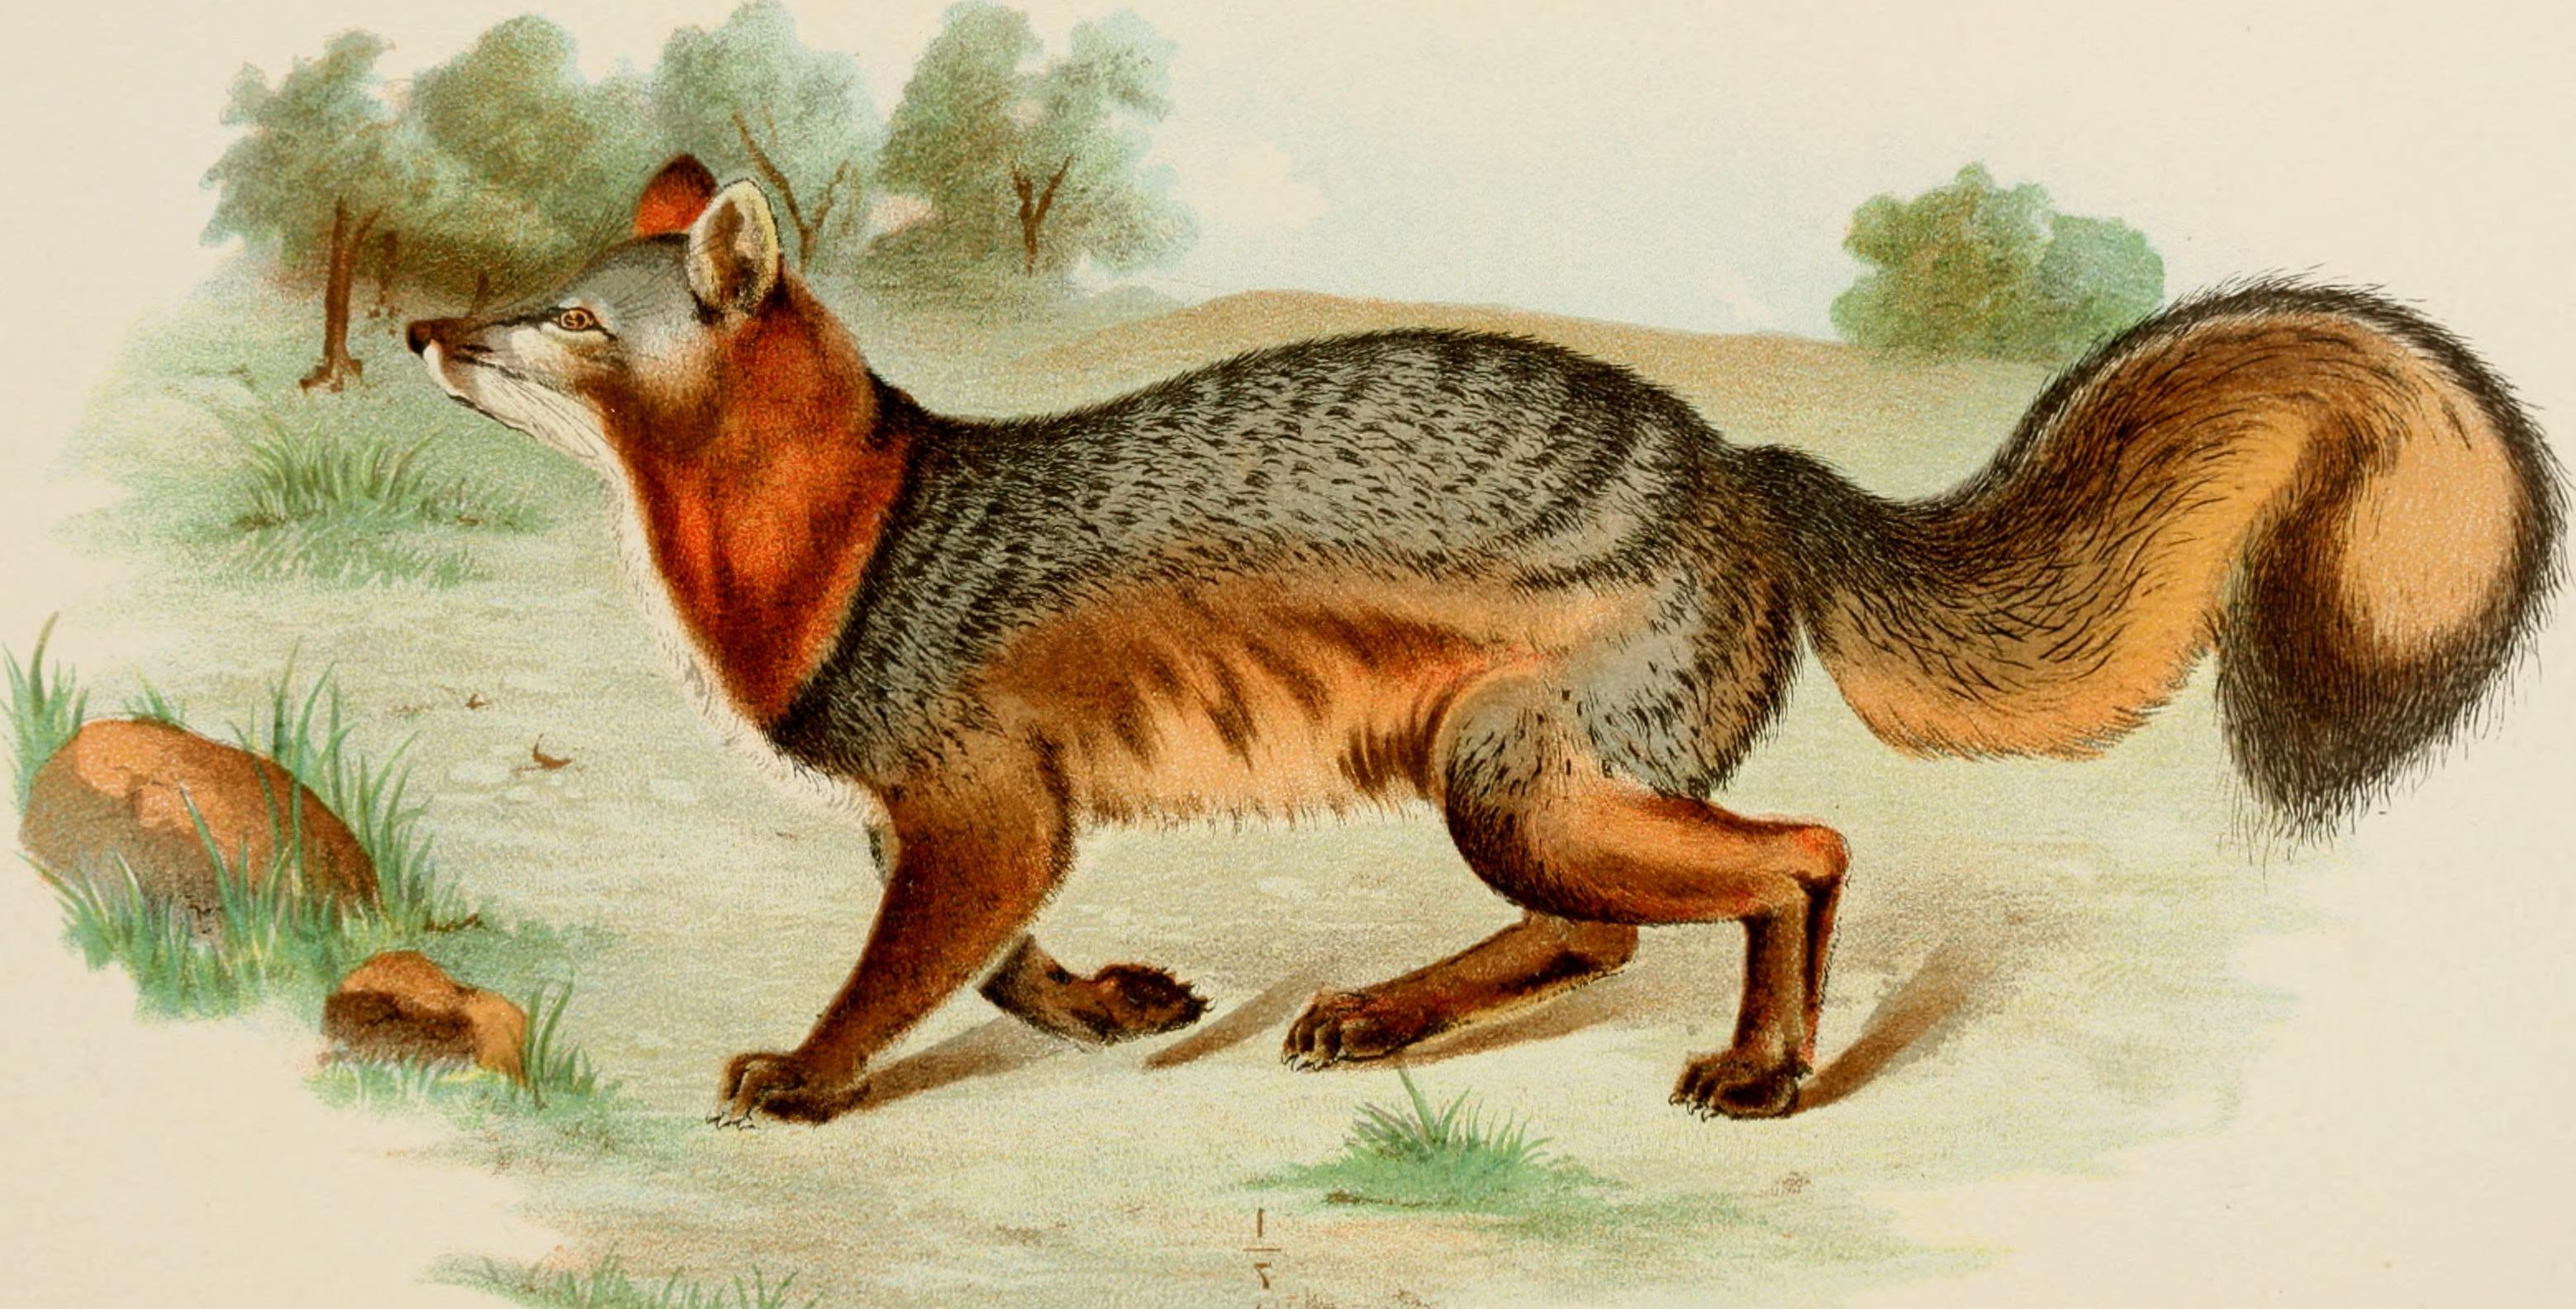
\includegraphics[width =
  \textwidth]{illustration_images/Quant_gen/Grey_fox/14770789583_4db7ec5164_o.jpg}  %https://www.flickr.com/photos/internetarchivebookimages/14770789583/in/photolist-axdicF-ovfa8V-odM3sY-bCrnQ8-ovgYXn-tiQfMQ-odMpu5-x1xCJu-wQ7qT7-wE7kfs-xEZQd1-wK4YSh-ovWx4g-wpDZzF-xjvQ89-tHDjuS-w9Wit5-xEvyhH-xjCbKD-u4q3Qe
\end{center}
\caption{Gray Fox, {\it Urocyon cinereoargenteiis}. Pearson and Warren. Diseases and enemies of poultry. (1897) BHL.} 
\end{marginfigure}

\marginnote{
\begin{question}
\citet{robinson:16} found that the endangered Californian Channel Island fox on San Nicolas had very
low levels of diversity ($\pi =0.000014 \text{bp}^{-1}$) compared to
its close relative the California mainland gray fox ($0.0012\text{bp}^{-1}$). \\
%\bf A How many sites do you expect to differ between two samples
%sequenced over a 100kb region in each of these populations?\\   
{\bf A)} Assuming a mutation rate of $2\times 10^{-8}$ what
effective population size do you estimate for these two populations?
\\
{\bf B)} Why is the effective population size of the Channel Island fox
so low? [Hint: quickly google Channel island foxes to read up on their
history, also to see how ridiculously cute they are.]
\end{question}
}

\paragraph{More details on the pairwise coalescent.}
\graham{This section is currently where some of the continuous time
  coal. has been moved.}


Conditional on the calescent time $t$ the probability of our pair of alleles are separated by $j$ mutations
since they last shared a common ancestor is
\begin{equation}
P(j | T_2 = t ) = {2t \choose j} \mu^{j} (1-\mu)^{2t-j}
\end{equation}
i.e. mutations happen in $j$ generations, and do not happen in $2t-j$
generations (with ${2t \choose j}$ ways this can possibly
happen). Assuming that $\mu \ll 1$, and that $2t-j \approx 2t$ then we
can approximate the probability that we have $j$ mutations as a
Poisson distribution
\begin{equation}
P(j | T_2 = t ) = \frac{ (2 \mu t )^{j} e^{-2\mu t}}{j!}
\end{equation}
i.e. a Poisson with mean $2\mu t $. \\


\section{The coalescent process of a sample of alleles.}

Usually we are not just interested pairs of alleles, or the
average pairwise diversity, we are interested in the properties of
diversity in samples of a number of alleles drawn from the population.  
To allow for this instead of just following a pair of lineages back until they
coalesce, we can follow the history of a sample of alleles back
through the population.

Consider first sampling three alleles at random from the population. The
probability that all three alleles choose exactly the same ancestral allele one
generation back is $\nicefrac{1}{(2N)^2}$. If $N$ is reasonably large then this
is a very small probability. As such it is very unlikely that our three alleles
coalesce at once, a in a moment we'll see that it is safe to ignore such
unlikely events. \\

\begin{figure}
\begin{center}
  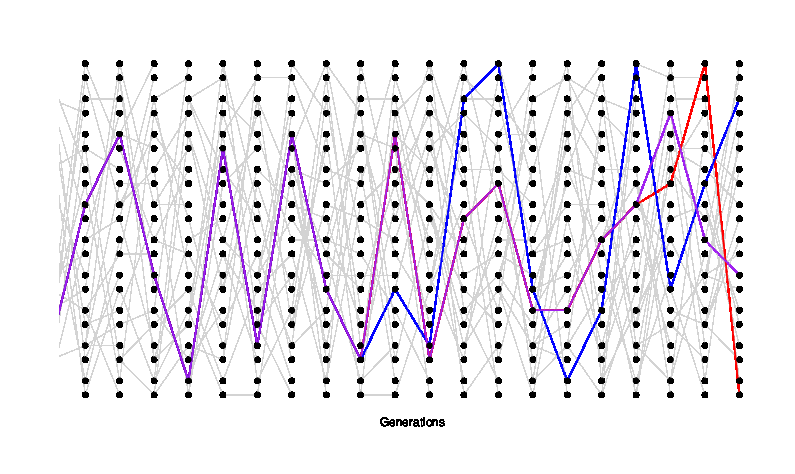
\includegraphics[width = \textwidth]{figures/Coalescent_3.png}
\end{center}
\caption{A simple simulation of the coalescent process for three
  lineages. We track the ancestry of 
  three modern-day alleles, the first pair (blue and purple) coalesce four generations back 
  their are then two independent lineages we are tracking, this pair
  then coalesces twelve generations in the past. Note that different
  random realizations of this process will differ from each other a lot.} \label{fig:Coalescent_simulation_3}
\end{figure}

The probability that a specific pair of alleles find a common ancestor in the
preceding generation is still $\nicefrac{1}{(2N)}$. There are three possible pairs of
alleles so the probability that no pair finds a common ancestor is
\begin{equation}
\left(1-\frac{1}{2N} \right)^3 \approx \left( 1- \frac{3}{2N} \right)
\end{equation}
in making this approximation we are multiplying out the right hand-side
and ignoring terms of $1/N^2$ and higher. See
Figure \ref{fig:Coalescent_simulation_3} for a random realization of this process. \\

More generally when we sample $i$ alleles there are ${i \choose 2}$
pairs,\sidenote{said as ``i choose 2''}  i.e. $i(i-1)/2$ pairs, thus the probability that no pair
of alleles coalesces in the preceding generation is
\begin{equation}
\left(1-\frac{1}{(2N)} \right)^{{i \choose
 2}} \approx \left( 1- \frac{{i \choose
 2}}{2N}\right)
\end{equation}
while the probability of any pair coalescing is $\approx \nicefrac{2N}{{i \choose
 2}}$.\\

We can ignore the possibility of more than pairs of alleles (e.g. tripletons)
simultaneously coalescing at once as terms of $\nicefrac{1}{N^2}$ and higher
can be ignored as they are vanishingly rare. Obviously there are in reasonable
sample sizes there are many more triples (${i \choose 3}$), and higher order
combinations, than pairs (${i \choose 2}$) but if $i \ll N$ then we are safe to
ignore these terms.

\marginnote{
To see the continuous time  version of this note that \eqref{eqn:T_i} is
\begin{equation} 
\approx  \frac{{i \choose
 2}}{2N} \exp \left( - \frac{{i \choose
 2}}{2N} t \right)
\end{equation}
the waiting time $T_i$ to the first coalescent event in a sample
of $i$ alleles is exponentially distributed with rate $\nicefrac{{i \choose
 2}}{2N}$, i.e. $T_i \sim \text{Exp}\left(\nicefrac{{i \choose
 2}}{2N} \right)$. }

When there are $i$ alleles the probability that we wait until the
$t+1$ generation before
any pair of alleles coalesce is
\begin{equation}
 \frac{{i \choose
 2}}{2N}\left( 1- \frac{{i \choose
 2}}{2N}\right)^{t} \label{eqn:T_i}
\end{equation}
thus the waiting time while there are $i$ lineages is a geometrically
distributed random variable with probability of success $ \nicefrac{{i \choose
    2}}{2N}$, which we denote by
\begin{equation}
T_i \sim \text{Geo}
\left(  \nicefrac{{i \choose
      2}}{2N} \right).
\end{equation}
The mean waiting time till any of pair within our
 sample to coalesce is 
\begin{equation}
\E( T_i) \frac{2N}{{i \choose  2}}  \label{eqn:E_T_i}
\end{equation}

When a pair of alleles first find a common ancestral allele some
number of generations back further into the past we only have to keep
track of that common ancestral allele for the pair. Thus when a pair
of alleles in our sample of $i$ alleles coalesce, we then switch to
having to follow $i-1$ alleles back. Then when a pair of these $i-1$
alleles coalesce, we then have to follow $i-2$ alleles back. This
process continues until we coalesce back to a sample of two, and from
there to a single most recent common ancestor (MRCA).\\


\paragraph{Simulating a coalescent genealogy}
To simulate a coalescent genealogy at a locus for a sample of $n$ alleles we therefore simply follow this
algorithm
\begin{enumerate}
\item Set $i=n$.
\item We simulate a random variable to be the time $t_i$ to the next coalescent event from $t_i \sim
  \text{Exp}\left(\nicefrac{{i \choose
 2}}{2N} \right)$
\item Choose a pair of alleles to coalesce at random from all possible
 pairs.
\item Set $i=i-1$
\item Continue looping of steps 1-3 until $i=1$ i.e. the most recent
 common ancestor of the sample is found.
\end{enumerate}
by following this algorithm we are generating realizations of the
genealogy of our sample. \\



\subsection{Expected properties of coalescent genealogies and
  mutations.} 

\begin{figure}
\begin{center}
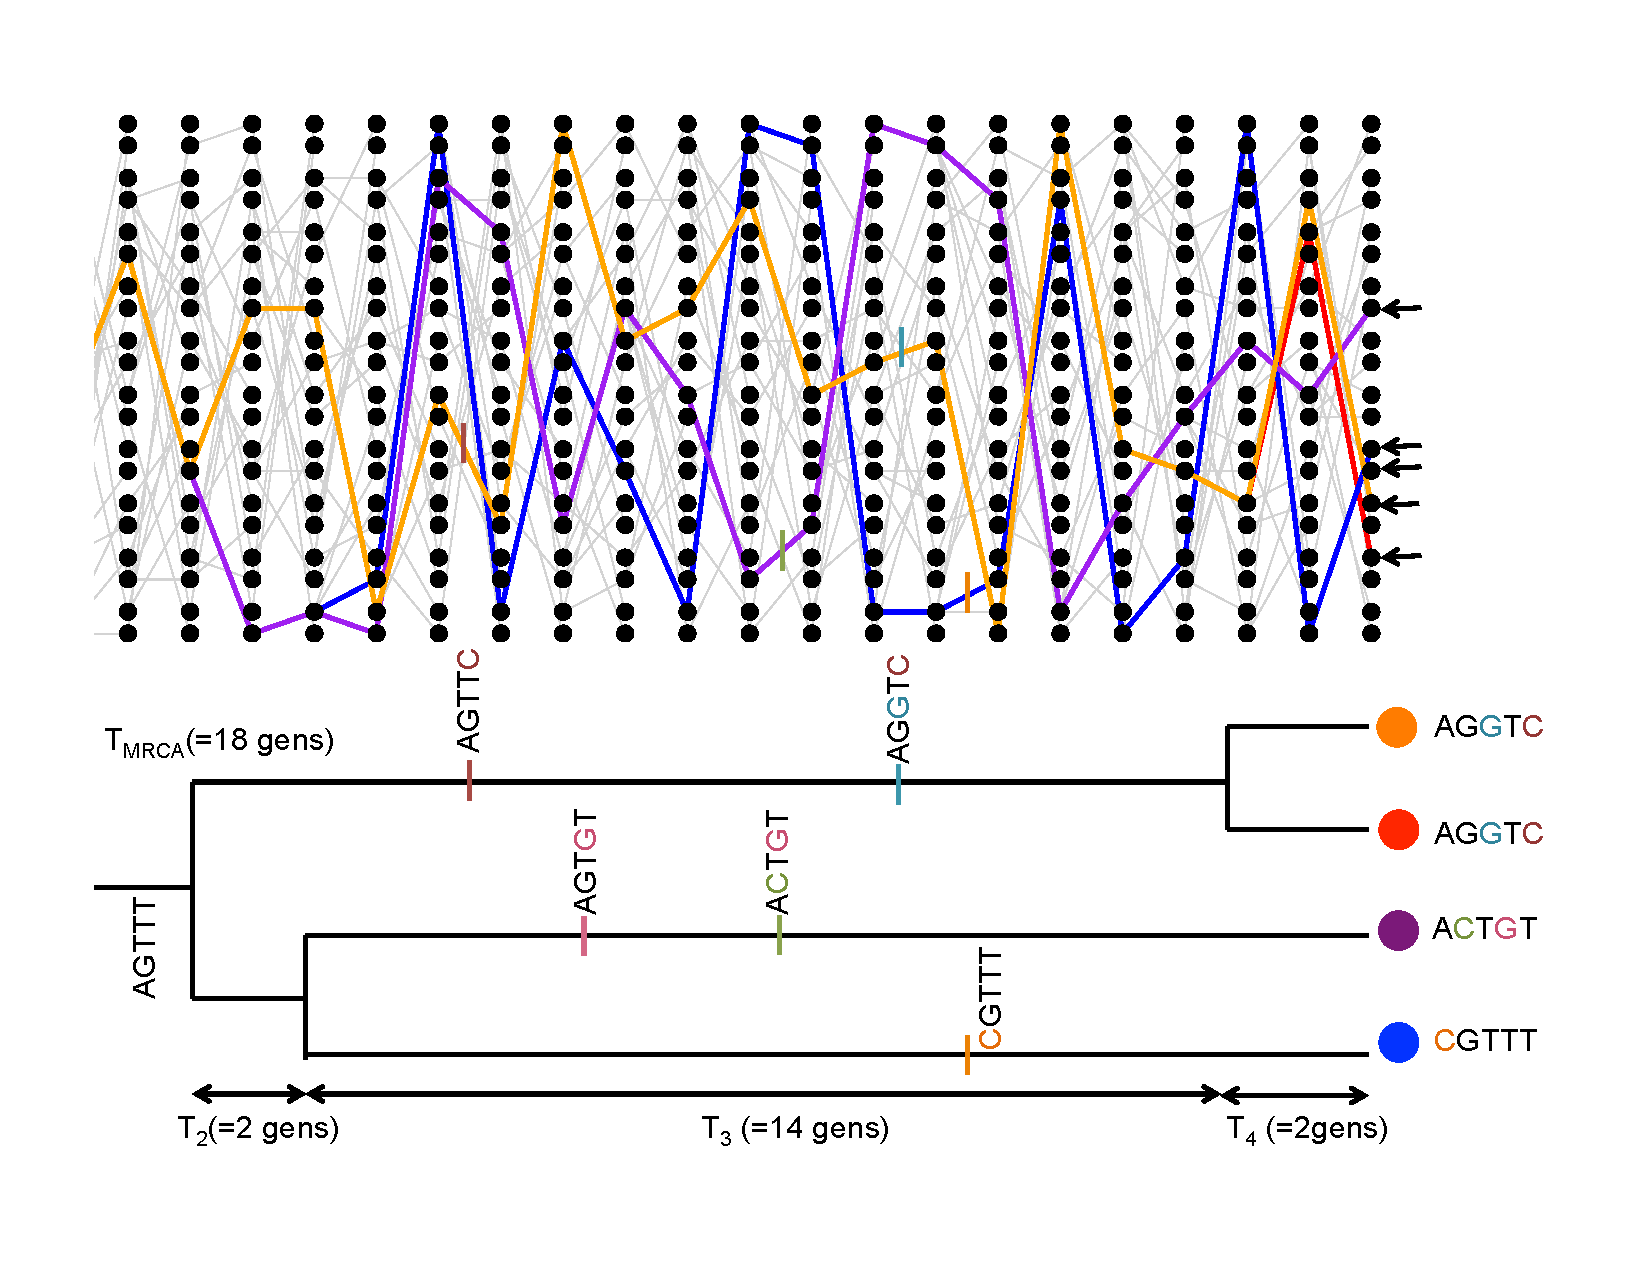
\includegraphics[width= \textwidth]{figures/Coalescent/Coal_w_muts.pdf}
\end{center}
\caption{ } \label{fig:Coal_w_muts}
\end{figure}


\paragraph{The expected time to the most recent common ancestor.}
We will first consider the time to the most recent common ancestor of
the entire sample ($T_{MRCA}$). This is
\begin{equation}
T_{MRCA} = \sum_{i=n}^2 T_i
\end{equation}
generations back. As our coalescent times for different $i$ are independent, the expected time to the most recent common ancestor
is
\begin{equation}
\E(T_{MRCA}) = \sum_{i=n}^2 \E(T_i) = \sum_{i=n}^2  2N/{i \choose
 2}
\end{equation}
using the fact that $\frac{1}{i(i-1)}=\frac{1}{i-1} - \frac{1}{i}$ with a bit of
rearrangement we can rewrite this is
\begin{equation} 
\E(T_{MRCA}) = 4N\left(1- \frac{1}{n} \right) \label{TMRCA_neutral}
\end{equation}
so the average $T_{MRCA}$ scales linearly with population
size. Interestingly, as we move to larger and larger samples (i.e. $n \gg 1$) the average
time to the most recent common ancestor is converging on $4N$. What's
happening here is that in large samples our lineages typically coalesce rapidly
at the start and very soon coalesce down to a much smaller number of
lineages.   \\


\paragraph{The expected total time in a genealogy and the number of
  segregating sites.}

Mutations fall on lineages of the coalescent genealogy. These mutations affect all
descendants of this lineage, and under the infinitely-many-sites assumption,
create a new segregating site for each new mutation. The mutation process is a
\emph{Poisson process}, and the longer a particular lineage branch, the more
mutations that can accumulate on it. The total number of segregating sites in
the genealogy is thus a function of the \emph{total} amount of time in the
genealogy of the sample, or the sum of all the genealogy branch lengths,
$T_{tot}$. Since our coalescent genealogies are bifurcating (only two lineages
coalesce at once), our total amount of time in the genealogy is:

\begin{equation}
T_{tot} = \sum_{i=n}^2 iT_i
\end{equation}
as when there are $i$ lineages each contributes a time $T_i$ to the
total time. Taking the expectation of the total time in the genealogy
\begin{equation}
\E(T_{tot}) = \sum_{i=n}^2 i \frac{2N}{{i \choose
 2} } = \sum_{i=n}^2 \frac{4N}{i -1} =\sum_{i=n-1}^1 \frac{4N}{i}
\end{equation}
so our expected total amount of time in the genealogy scales linearly
with our population size. Our expected total amount of time is also
increasing with sample size but is doing so very slowly. To see this
more carefully we can see that for large $n$
\begin{equation}
\E(T_{tot}) = \sum_{i=n-1}^1 \frac{4N}{i} \label{eqn:E_T_tot}
\end{equation}
\marginnote{To get a better sense of how this grows with the sample we
  can see that \ref{eqn:E_T_tot} can be approximated by $\int_1^n \frac{1}{i} di
= 4N \log(n-1)$ approximating our sum by an integral, which will work for
large $n$. }
So our expected total amount of time in the genealogy
is growing with $n$ but it is doing so very slowly. This again follows
from the fact that in large samples the initial coalescence usually
happens very rapidly, so that extra samples adds little to the total
amount of time in the tree. \\

We saw above that the number of mutational differences between a pair
of alleles that coalescence $T_2$ generations ago was Poisson with a
mean of $2 \mu T_2$. A mutation that occurs on any branch of our
genealogy will cause a segregating polymorphism in the sample
(making our infinitely-many-sites assumption). Thus if the total time
in the genealogy is $T_{tot}$ there is $T_{tot}$
generations for mutations. So the total number of mutations
segregating in our sample ($S$) is Poisson with mean $\mu T_{tot}$. Thus the
expected number of segregating in history a sample of size $n$ is
\begin{equation}
\E(S) = \mu \E(T_{tot}) = \sum_{i=n-1}^1 \frac{4N\mu }{i} = \theta
\sum_{i=n-1}^1 \frac{1}{i}
\end{equation}
Thus we can use this formula to derive another estimate of the
population scaled mutation rate, by setting our observed number of
segregating sites in a sample ($S$) equal to this expectation. We'll call this estimator $\widehat{\theta}_W$
\begin{equation}
\widehat{\theta}_W =\frac{ S}{\sum_{i=n-1}^1 \frac{1}{i}}  
\end{equation}
this estimator was devised by \citeauthor{watterson:75}\cite{watterson:75}, hence the $W$.


\paragraph{The neutral site-frequency spectrum.}

We can use our coalescent process to find our the expected number of
alleles present $i$ times out of $n$, e.g. how many singletons do we
expect to find in our sample?  

\begin{marginfigure}
\begin{center}
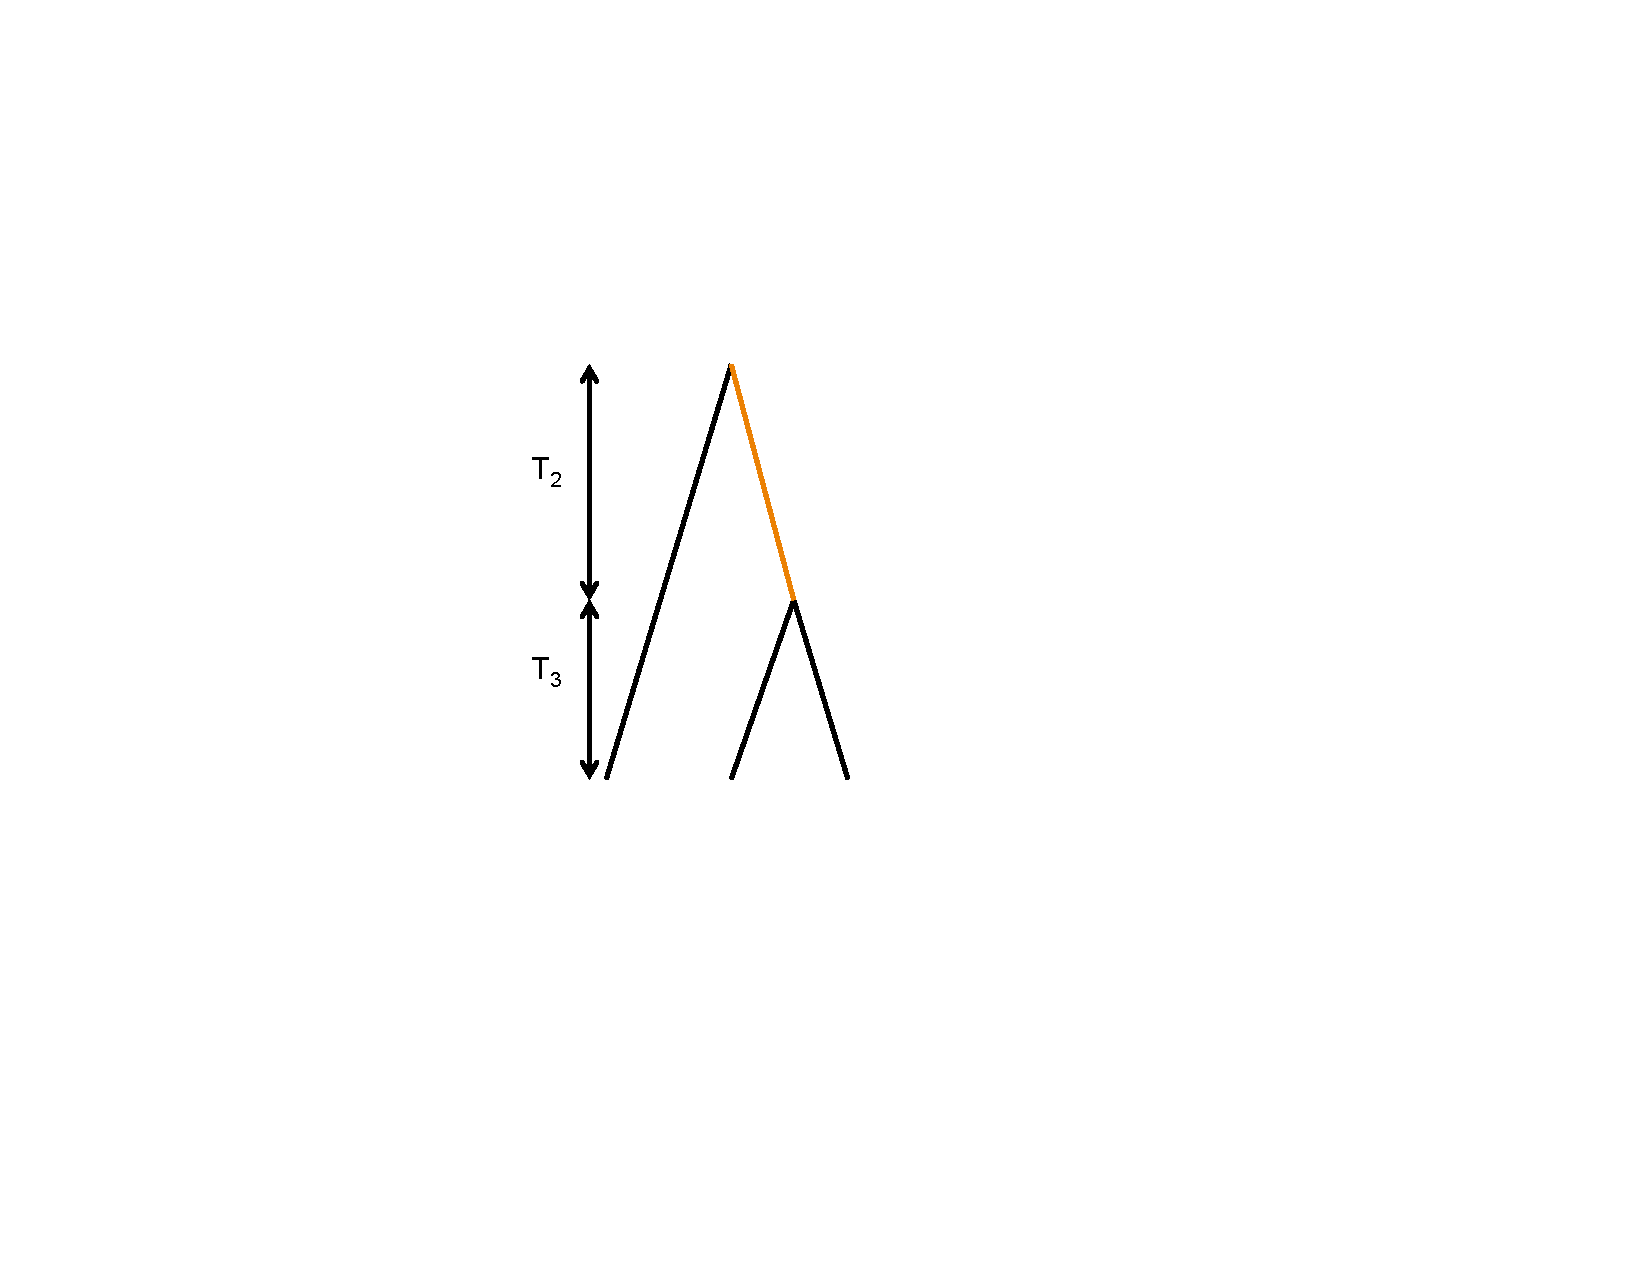
\includegraphics[width= \textwidth]{figures/Genetic_drift/freq_spec_tree.pdf}
\end{center}
\caption{A tree for three samples, note that this is the only possible
tree shape (treating the tips as unlabelled)} \label{fig:freq_coal}
\end{marginfigure}

To see how we could go about working this out, lets start by
considering the coalescent tree, shown in \ref{fig:freq_coal}, for sample of $3$ alleles drawn from a
population. Mutations that fall on the
branches coloured in black will be derived singletons, while mutations that
fall along the orange branch will be doubletons in the sample. The
total number of generations where a singleton mutation could arise is
$3 T_3 + T_2$, note that we only count the time where there are two
lineages once. While the time where doubletons could arise is
$T_2$. So our expected number of singletons, using eqn \eqref{eqn:E_T_i}, is 
\begin{equation}
\E(S_i) = \mu \left( 3\E(T_3) +  \E(T_3) \right) = \mu \left( 3
  \frac{2N}{3}+ 2N \right) = \theta
\end{equation}
by similar logic our expected number of doubletons is $\E(S_i)
=\theta/2$, i.e. there are half as many doubletons as singletons. 

Extending this logic to large samples is doable, but tedious
\graham{Give  numbers for 10 tips}. A nice
simple proof of the neutral site frequency spectrum is given by
\citeauthor{Hudson:15}, but we won't give this here. The general form is: 
\begin{equation}
\E(S_i) = \theta \frac{1}{i}   \label{eqn:neutral_freq_spec}
\end{equation}
there are twice as many singletons as doubletons, three times as many
singletons as tripletons, and so on. The other thing that will be
helpful for us to know is that neutral alleles at intermediate frequency tend to be old, and
those that are rare in the sample are young.

\begin{question}
There are two possible tree shapes that could relate four
samples. Colour (or otherwise mark) the branches by where singletons,
doubletons, and tripleton derived alleles could arise. 

Can you work out the expected number of each types of allele?
\end{question}


\paragraph{tests based on the site frequency spectrum}
A variety of tests of whether site frequency spectrum conforms to its
neutral, constant-population expectations have been proposed. This is
useful for detecting population size changes using many loci data, or
for detecting the signal of selection at individual loci. One of
the first was proposed by \citeauthor{tajima:89}, and is called
Tajima's $D$. Tajima's $D$ is
\begin{equation}
  D = \frac{\theta_{\pi}-\theta_{W}}{C} \label{eqn_Tajimas_D}
\end{equation}
where the numerator is the difference between the estimate of
$\theta$ based on pairwise differences and that based on segregating
sites. As these two estimators both have expectation $\theta$ under
the neutral, constant-population model the expectation of $D$ is zero. The denominator $C$ is the square-root of an estimator
variance of this difference, the idea being for $D$ to have mean zero
and variance $1$. \\

An excess of rare alleles compared to the constant-population, neutral
model will result in the negative Tajima's $D$, because each
additional rare allele increases the number of segregating sites by
$1$, but only has a small effect on the pairwise differences. 
A positive Tajima's $D$ reflects an excess of intermediate frequency alleles, relative to
the  constant-population, neutral model. As intermediate-frequency, neutral alleles increase pairwise diversity
more per segregating site than a typical neutral alleles.


\subsection{Demography and the coalescent}

\begin{marginfigure}
\begin{center}
  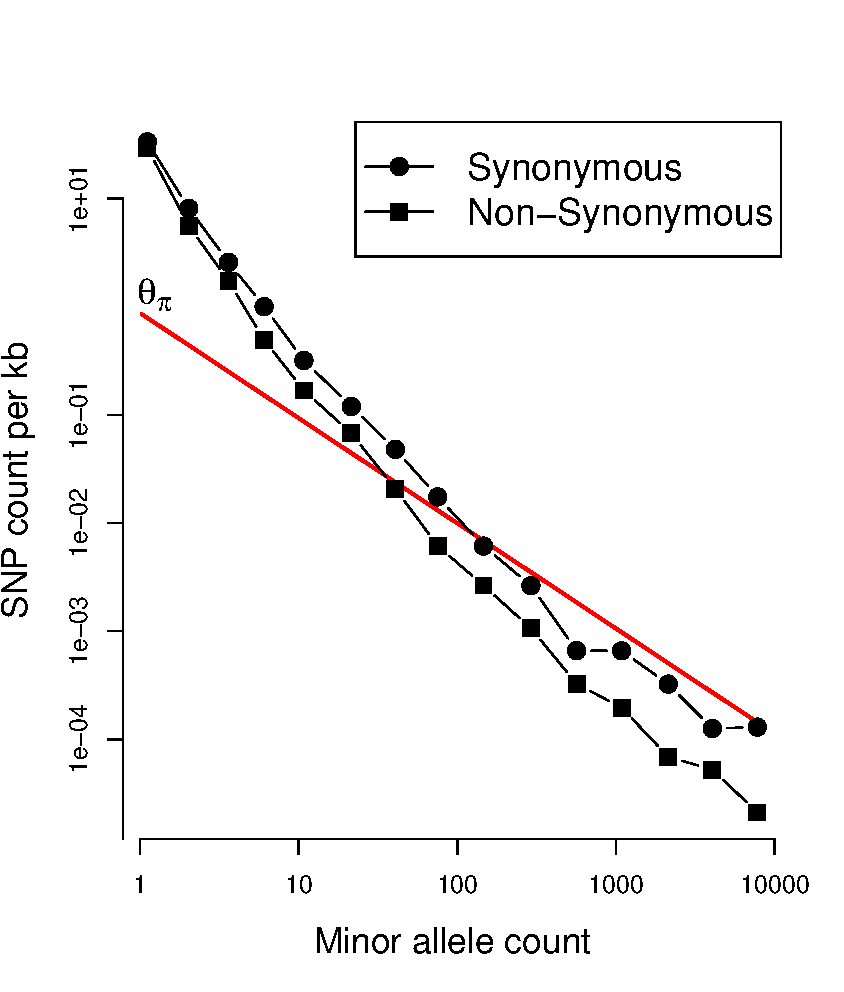
\includegraphics[width = \textwidth]{Journal_figs/genetic_drift/human_pop_growth/Nelson_pop_growth.pdf}
\end{center}
\caption{Data from 202 genes from 14002 people of European ancestry (28004 alleles). Note
  the double log-scale. Redrawn from citeauthor{nelson:12}. The red
  line gives the neutral, constant population size estimate using a
  $\theta$ estimated from $\pi$.} \label{fig:Human_growth}
\end{marginfigure}
We've already seen how changes in population size can change the rate
at which heterozygosity is lost from the population (see the
discussion around eqn. \eqref{eqn:var_pop_coal}). If the population
size in generation $i$ is $N_i$ the probability that a pair of
lineages coalesce is $\nicefrac{1}{2N_i}$, this conforms to our
intuition that if the population size is small that the rate at which
pairs of lineages find their common ancestor is faster. If the
population randomly fluctuates rapidly in size throughout 
we can often accomodate this simply by using the effective popuation size $N_e$ in place of $N$. However,
longer term more systematic changes in population size will distort
the coalescent genealogies, and hence patterns of diversity, in more
systematic ways. 

As an example of how demography can potentially distort patterns left
in a sample the observed frequency spectrum from a very large sample of humans, shown in Figure \ref{fig:Human_growth}. For
comparison the neutral frequency spectrum, eqn
\eqref{eqn:neutral_freq_spec}, is shown as a red line. There are
  vastly more rare alleles than expected under our neutral, constant-population-size model. 

\begin{figure}
\begin{center}
  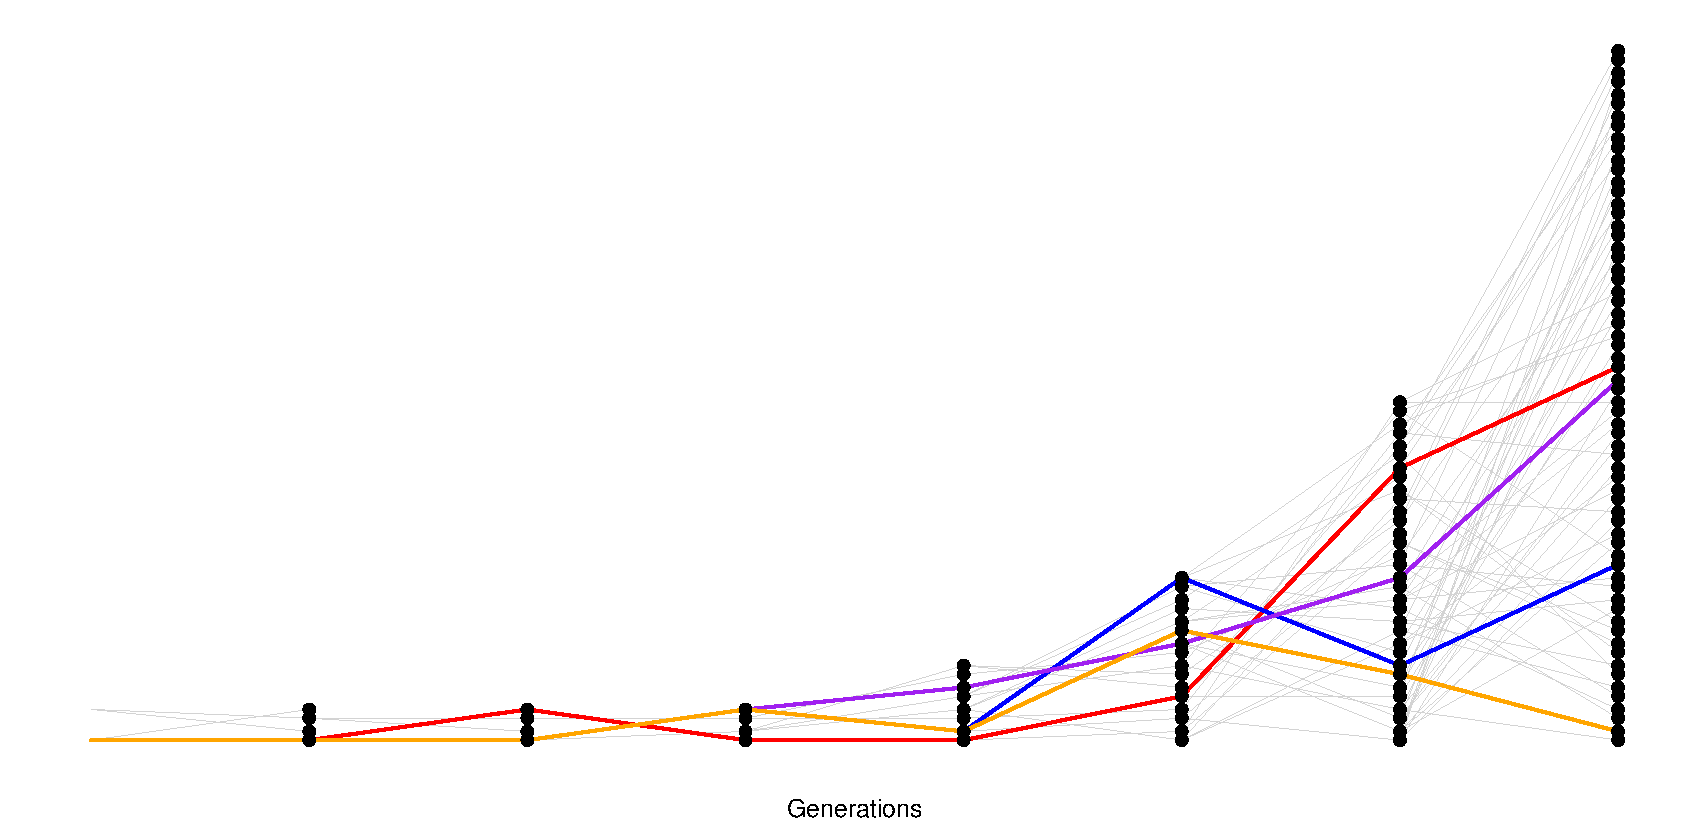
\includegraphics[width = \textwidth]{figures/Genetic_drift/Demography/Growth_genealogy.pdf}
\end{center}
\caption{} \label{fig:Genealogy_growth}
\end{figure}

Why is this? Well this is likely the result of the very recent
explosive growth in human populations. If the population has grown rapidly then the pairwise-coalescent
rate in the past may be much higher than closer to the present. (see Figure \ref{fig:Genealogy_growth}). 

The first consequence of this is that they'll be much less genetic
diversity in the population than you'd predict using the census
population size. One example of this is in humans, there's $7$ billion
of us alive today, but this is due to very rapid population growth
over the past thousand to tens of thousands of years. Our level of
genetic diversity is very much lower than you'd predict given our
census size. The second consequence is that the deeper coalescent branches are
much more squished together in time, compared to those in a constant
population.  These deeper branches are the source of alleles at more
intermediate frequency, and so there are even fewer of these alleles
in growing populations. That's why there are so many rare alleles,
especially singletons in this large sample of Europeans. 


Another common demographic scenerio is a population population
neck. Here the population size crashes dramatically, and subsequently
recovers. For example our population may have size $N_{\textrm{Big}}$
and have crashed down to $N_{\textrm{Small}}$, one example of a
bottleneck is shown in Figure \ref{fig:Genealogy_crash}. 
\begin{figure}
\begin{center}
  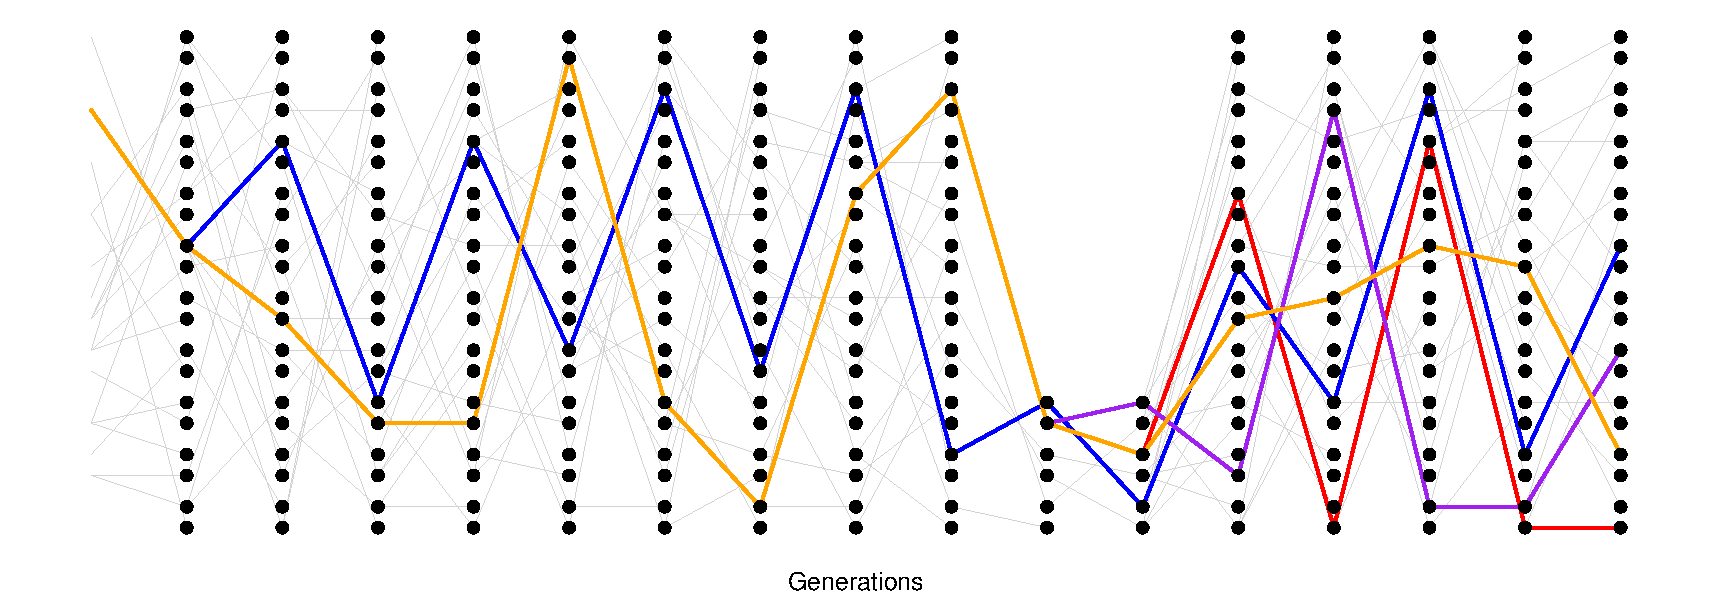
\includegraphics[width = \textwidth]{figures/Genetic_drift/Demography/Crash_genealogy.pdf}
\end{center}
\caption{} \label{fig:Genealogy_crash}
\end{figure}
Looking at a sample of lineages drawn from the population today, if
the bottleneck was somewhat recent, $\ll N_{\textrm{Big}}$ generations
in the past, many of our lineages will not have coalesced by the time
the bottleneck moving backward in time. But during the bottleneck our
lineages coalesce at a much higher rate, such that many of our
lineages will coalesce if the bottneck lasts long enough
($\sim N_{\textrm{Small}}$ generations). If the bottleneck is very
strong then all of our lineages will coalesce during it, and this may
look very like our population growth model (with an excess of rare
alleles). However, if some pairs of lineages escape coalescing during
the bottleneck they will coalesce much more deeply in time (e.g. the
blue and orange ancestral lineages in
\ref{fig:Genealogy_crash}). 
\begin{figure}
\begin{center}
  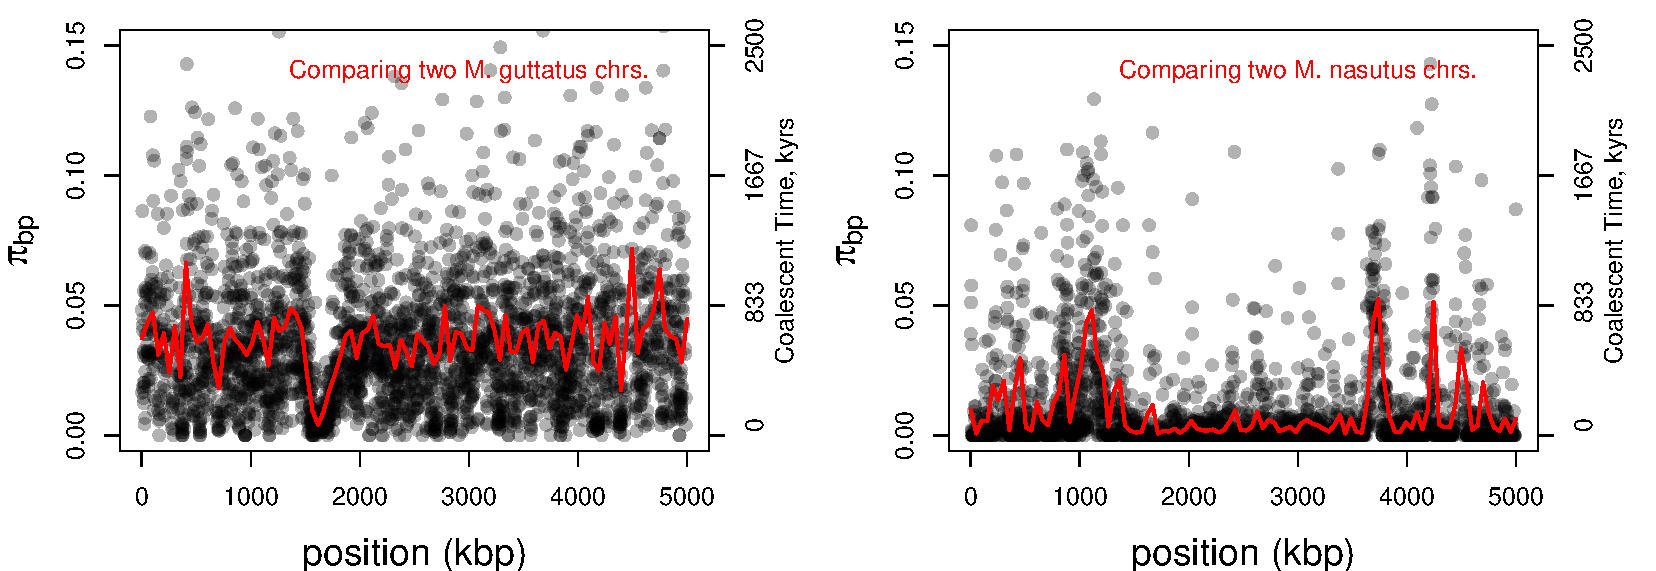
\includegraphics[width = \textwidth]{figures/Genetic_drift/Demography/Mimulus_coalescent_times.pdf}
\end{center}
\caption{Black dots give $\pi$ in 1kb windows, the red line is a
  moving average (data from  \citeauthor{brandvain:14}). Pairwise coalescent times ($t$) estimated assuming $\pi = 2 t
  \mu$m using $\mu_{BP}=10^{-9}$.} \label{fig:Mimulus_bottleneck}
\end{figure}
An example of this is shown Figure
\ref{fig:Mimulus_bottleneck}, data from \citeauthor{brandvain:14}. {\it Mimulus nasutus} is a selfing
species that arose recently from out-crossing progenitor {\it M.
  guttatus}, and experienced a strong bottleneck. {\it M. guttatus} has a very high levels of genetic diversity
($\pi=4\%$ at synonymous sites), but {\it M. nasutus} has lost much 
of this diversity ($\pi =1\%$). Looking along the genome, between a
pait of {\it M. guttatus} chromosomes, levels of
diversity are fairly uniformly high.
\begin{marginfigure}
\begin{center}
  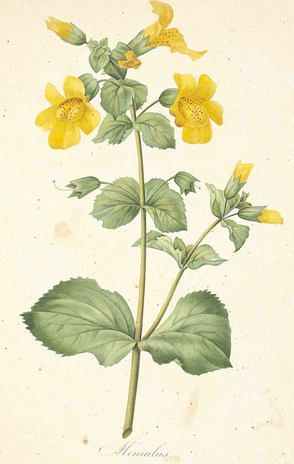
\includegraphics[width = 0.75 \textwidth]{illustration_images/Genetic_drift/Mimulus/Mimulus.png}
\end{center}
\caption{{\it M. guttatus} by Pierre-Joseph
  Redout\'e.} \label{fig:Human_growth}  %é
\end{marginfigure}
 But in comparing two {\it
  M. nasutus} diversity is low because the pair of lineages coalesce
recently; in a few places we see levels of diversity comparable to
{\it M. guttatus}, these regions correspond to our pair of lineages
failing to coalesce during the bottleneck and subsequently coalescing
much more deeply in the ancestral {\it M. guttatus} population.


Mutations that arise on these deeper lineages will be at intermediate frequency in our sample, and so mild bottlenecks
can lead to an excess of intermediate frequency alleles compared to
the standard constant-population model. This can result in skew 
Tajima's D, see eqn \ref{eqn_Tajimas_D}, towards positive values and away from its expectation of
zero . One example of this skew is shown in Figure
\ref{fig:maize_Tajimas_D}. Maize ({\it Zea mays}) was domesticated
  from its wild progenitor teosinte ({\it Z. }) roughly ten thousand years ago. We can see how the
 bottleneck associated with domestication as resulted in a loss of
 genetic diversity in maize and a skew
 towards intermediate frequency polymorphisms and so more positive
 values of Tajima's D.


\begin{figure}
\begin{center}
  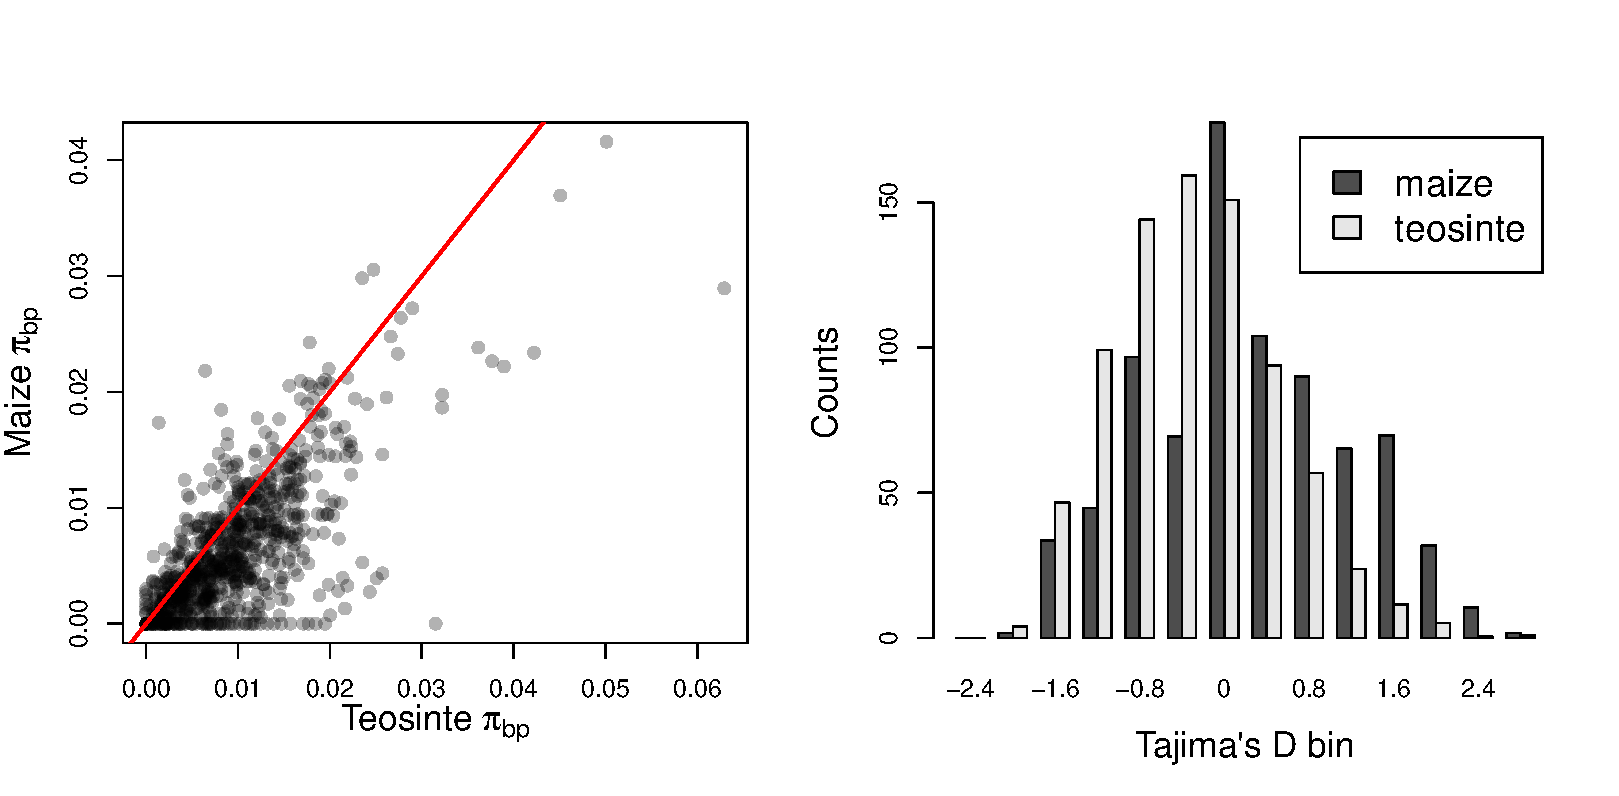
\includegraphics[width = 0.75 \textwidth]{Journal_figs/genetic_drift/Maize_bottleneck/Wright_Tajima_D.pdf}
\end{center}
\caption{Data for polymorphism from Maize and Teosinite 774
  genes redrawn from \citeauthor{Wright:05}{\bf Left)} Genetic
  diversity levels in maize and and Teosinte at each of these genes.
Note how diversity levels are lower in maize than teosinte, i.e. most
points are below the red $x=y$ line.  
. {\bf Right)}The distribution of Tajima's D in maize and teosinte. } \label{fig:maize_Tajimas_D}  %é
\end{figure}

\begin{marginfigure}
\begin{center}
  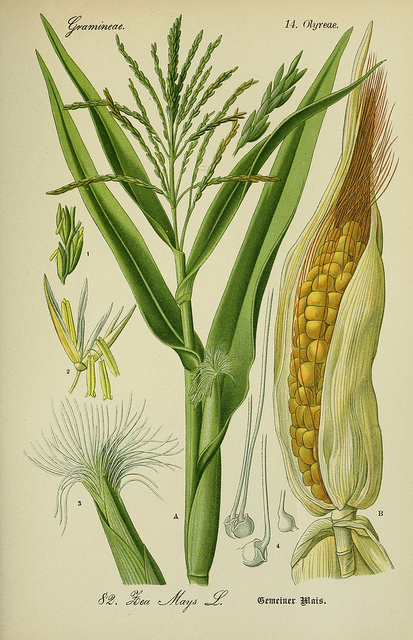
\includegraphics[width = \textwidth]{illustration_images/Genetic_drift/maize/7845339168_66aa3d8ccc_z.jpg}
\end{center}
\caption{Maize ({\it Zea mays}.) Prof. Dr. Thomé's Flora von
  Deutschland. 1886. Thomé, O. W. } \label{fig:maize}  %é
\end{marginfigure}



\section{Molecular Evolution and the fixation of neutral alleles} 
It is very unlikely that a rare
neutral allele accidentally drifts up to fixation; more likely, such an allele
will be eventually lost from the population. However, populations experience a
large and constant influx of rare alleles due to mutation, so even if it is
very unlikely that an individual allele fixes within the population, some
neutral alleles will fix by chance.  \\


%We'll first consider the probability that a neutral allele fixes
%within the population, starting from it just enters a diploid
%population as a newly mutated allele at frequency $1/(2N)$.

%so for an allele to be fixed in the population it
%must have been that allele

\paragraph{Probability of the eventual fixation of a neutral allele}
% TODO: tried to clean up this section, needs more work
An allele which reaches fixation within a population is an ancestor to the
entire population. In a particular generation there can be only single allele
that all other alleles at the locus in later generation can claim as an
ancestor. A neutral locus, the actual allele does not affect the number of
descendents that the allele has (this follows from the definition of
neutrality: neutral alleles don't leave more or less descendents on average).
An equivalent way to state this is that the allele labels don't affect
anything; thus the alleles are \emph{exchangeable}. As a consequence of this,
any allele is equally likely to be the ancestor of the entire population.  In a
diploid population size of size $N$, there are $2N$ alleles all of which are
equally likely to be the ancestor of the entire population at some later time
point. So if our allele is present in a single copy, the chance that it is the
ancestor to the entire population in some future generation is
$\nicefrac{1}{(2N)}$, i.e. the chance our neutral allele is eventually fixed is
$\nicefrac{1}{(2N)}$.  See Figure \ref{fig:subs_simulation}, our orange allele
in the first generation is one of 10 differently coloured alleles, and so has a
$1/10$ chance of being the ancestor of the entire population at some later time
point (as it is by the 9th generation).\\

More generally if our neutral allele is present in $i$ copies in the
population, of $2N$ alleles, the probability that this allele is fixed is
$\nicefrac{i}{(2N)}$, i.e. the probability that a neutral allele is eventually
fixed is simply given by its frequency ($p$) in the population.  (We can also
derive this result by letting $Ns \rightarrow 0$ in eqn.
\eqref{eqn:prob_fixed}, a result we'll encounter later.)

\begin{figure}
\begin{center}
  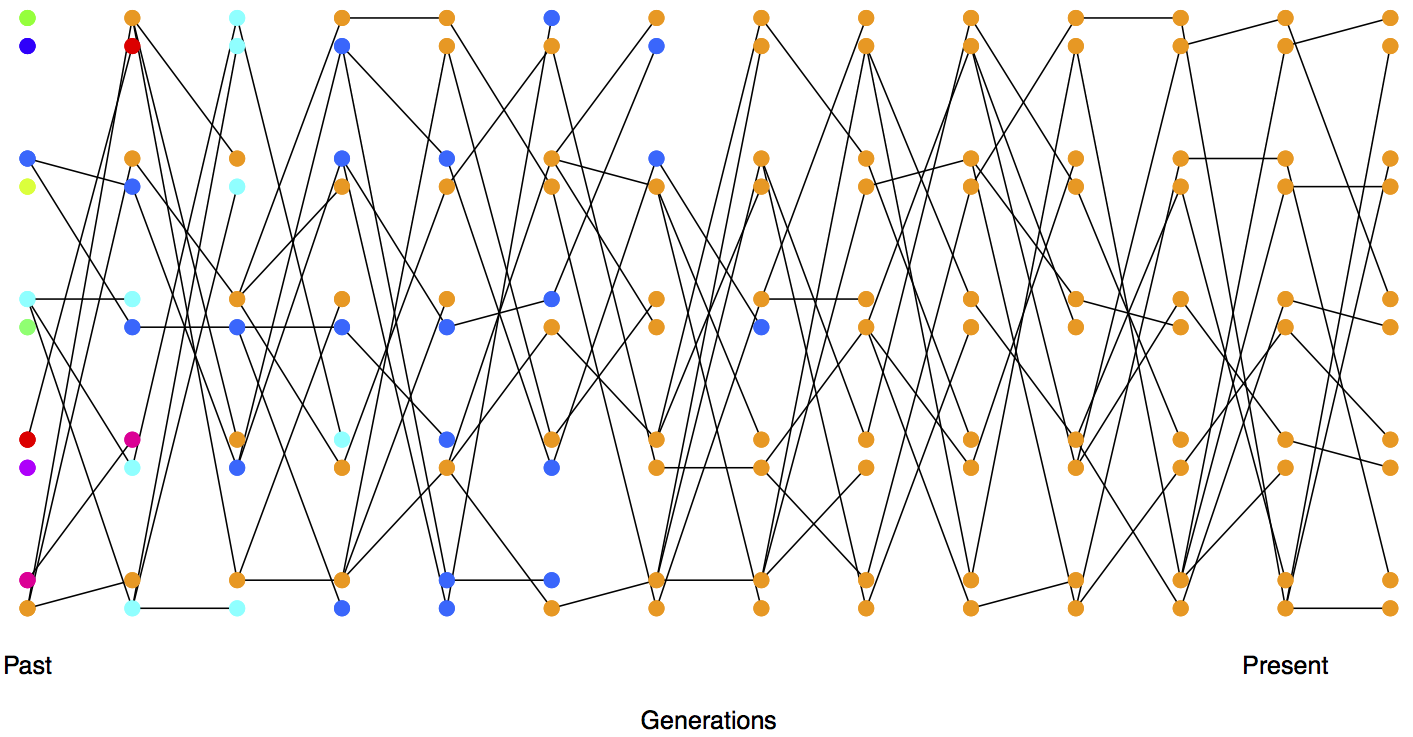
\includegraphics[width = \textwidth]{figures/Substitution_sim.png}
\end{center}
\caption{Each allele initially present in a small diploid population is
  given a different colour so we can track their descendants over
  time. By the 9th generation all of the alleles present in the
  population can trace their ancestry back to the orange allele.} \label{fig:subs_simulation}
\end{figure}


% TODO
An allele newly arisen mutation only becomes a fixed difference if it is lucky
enough to be the ancestor of the entire population. As we saw above this occurs
with probability $\nicefrac{1}{(2N)}$. How long does is take on average for
such an allele to fix within our population? Well in developing
equation \eqref{TMRCA_neutral} we've seen that it takes $4N$
generations for a large sample of alleles to all trace their ancestry back to a
single most recent common ancestor. Thus it must take roughly $4N$ generations
for a neutral allele present in a single copy within the population to the
ancestor of all alleles within our population. This argument can be made more
precise, but in general we would still find that it takes $\approx 4N$
generations for a neutral allele to go from its introduction to fixation with
the population.   \\

\paragraph{Rate of substitution of neutral alleles}

A substitution between populations that do not exchange gene flow is simply a
fixation event within one population. The rate of substitution is therefore the
rate at which new alleles fix in the population, so that the long-term
substitution rate is the rate at which mutations arise that will eventually
become fixed within our population.\\

Assume that there are two classes of mutational changes that can occur with a
region, highly deleterious mutations and neutral mutations. A fraction $C$ of
all mutational changes are highly deleterious, and can not possibly contribute
to substitution nor polymorphism (i.e. $Ns \gg 1$).  The other $1-C$ fraction
of mutations are neutral. If our mutation rate is $\mu$ per transmitted allele
per generation, then a total of $2N \mu (1-C)$ neutral mutations enter our
population each generation.\\

Each of these neutral mutations has a $\nicefrac{1}{(2N)}$ probability chance of
eventually becoming fixed in the population. Therefore, the rate at
which neutral mutations arise that eventually become fixed within our
population is  
\begin{equation}
2N\mu(1-C)\frac{1}{2N} = \mu(1-C)
\end{equation}
thus the rate of substitution under a model where newly arising alleles are either
highly deleterious or neutral, is simply given by the mutation rate
towards neutral alleles, i.e. $\mu(1-C)$.\\

Consider a pair of species have diverged for $T$ generations, i.e. orthologous sequences shared between the species last shared a common ancestor $T$ generations ago. If they have maintained a constant $\mu$ over that time, will have accumulated an average of
\begin{equation}
2\mu(1-C)T
\end{equation}
neutral substitutions. This assumes that $T$ is a lot longer than the time it
takes to fix a neutral allele, such that the total number of 
alleles introduced into the population that will eventually fix is the
total number of substitutions. We'll see below that a neutral allele
takes on average $4N$ generations to fix from its introduction into
the population.\\

This is a really pretty result as the population size has completely canceled
out of the neutral substitution rate. However, there is another way to see this
in a more straight forward way. If I look at a sequence in me compared to say a
particular chimp, I'm looking at the mutations that have occurred in both of
our germlines since they parted ways $T$ generations ago. Since neutral alleles
do not alter the probability of their transmission to the next generation, we
are simply looking at the mutations that have occurred in $2T$ generations
worth of transmissions. Thus the average number of neutral mutational
differences separating our pair of species is simply $2\mu (1-C) T$.\\

\begin{marginfigure}
\begin{center}
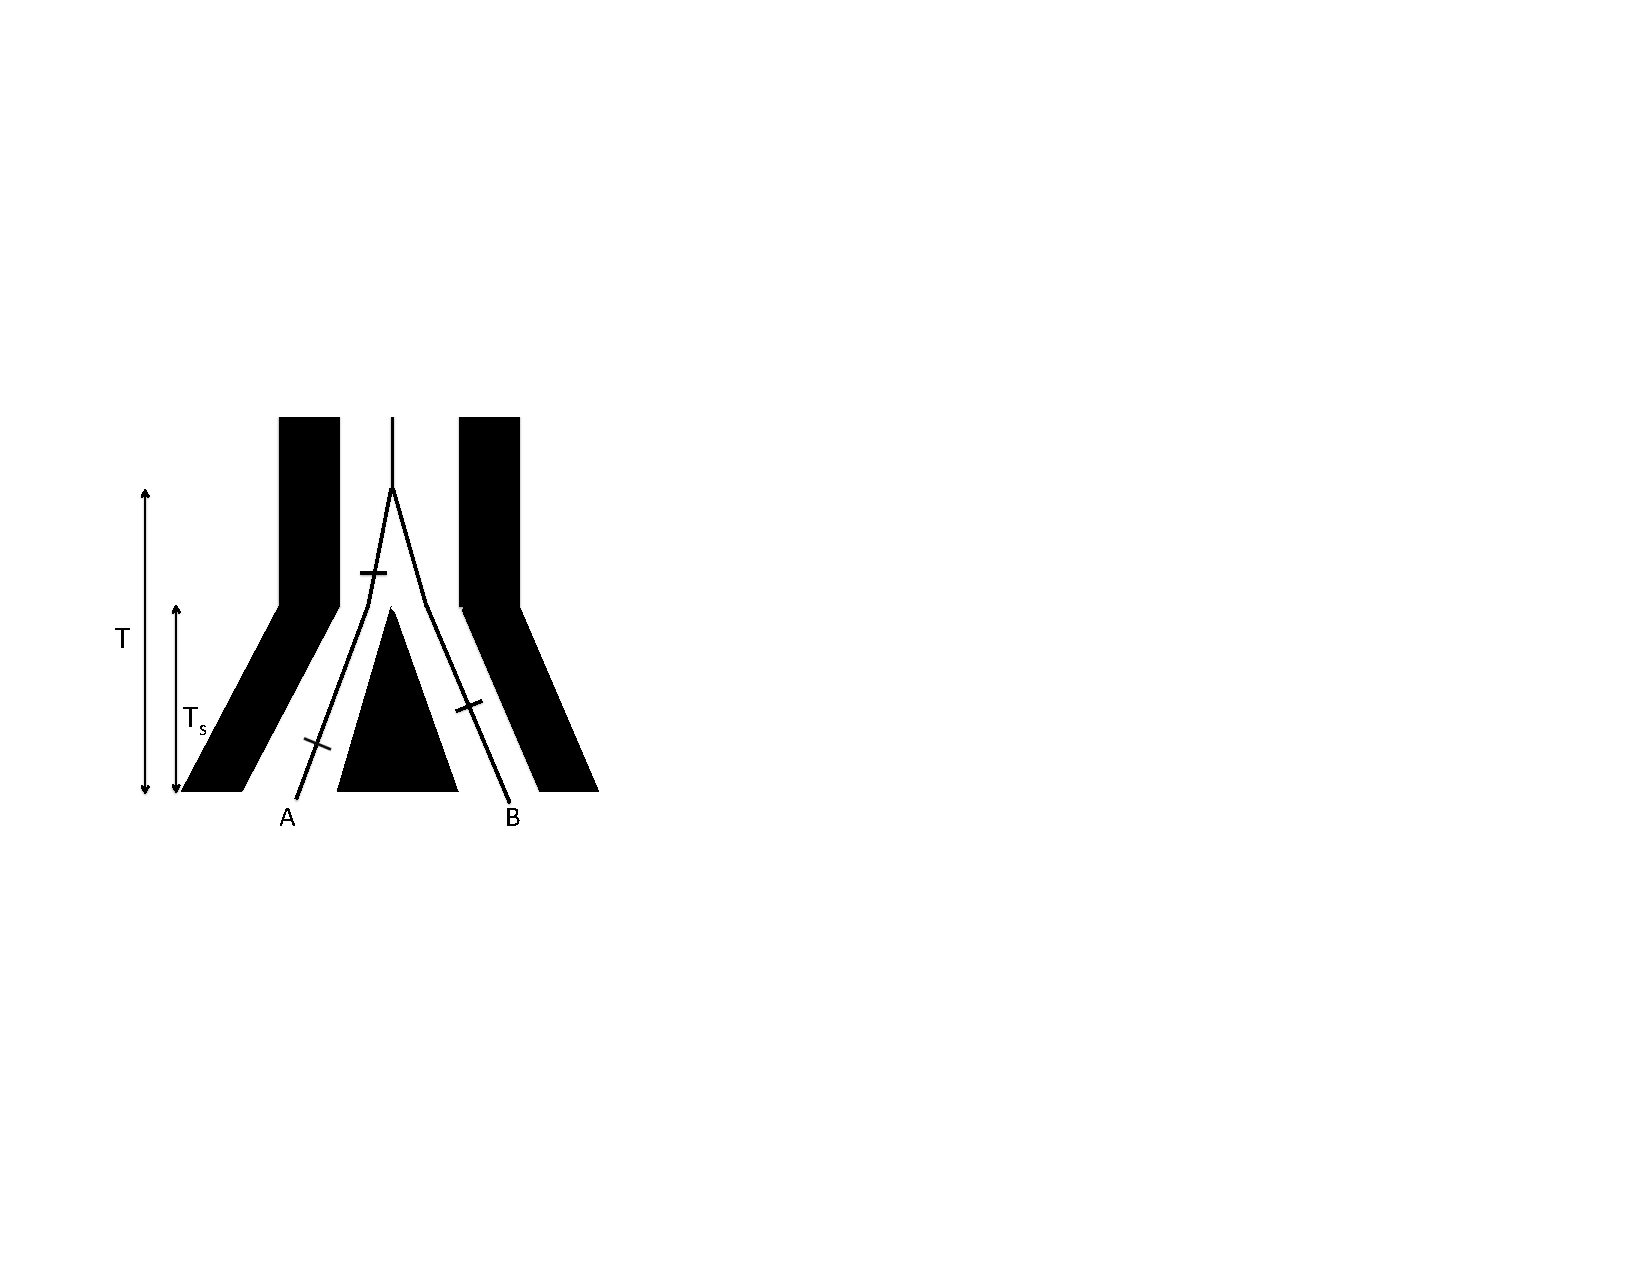
\includegraphics[width=0.8 \textwidth]{figures/Genetic_drift/ILS/split_anc_pop.pdf}
\end{center}
\caption{} \label{fig:split_anc_pop}  
\end{marginfigure} 


If we are considering $T$ to represent the divergence between long
separated species, then we can think of $T$ as the time that the
species split. However, for more recently diverged populations and
species, we need to include the fact that the sorting of ancestral
polymorphism contributes to divergence among species. In Figure 
\ref{fig:split_anc_pop}, we see a lineage selected from population A
and B, with three mutations that separate them shown as dashes. Our two populations split $T_s$ generations ago.  However, the
coalescence of our A and B lineage is necessarily deeper in time than
$T_s$. The top mutation was polymorphic in the ancestral population
but now contributes to the divergence between A and B. Assuming that
our ancestral population had effective size of $N_A$ individuals, and
that our populations split cleanly with no subsequent gene flow, then
\begin{equation}
T = T_s + 2N_A.
\end{equation}
Therefore, polymorphism in the ancestral population can make up a
sizable proportion of the divergence between closely related
species/populations. \graham{lineup split time in this section w. FST section.}



\begin{question}
For this, and the next question, assume that humans and chimp diverged
\graham{Update numbers?}
around 5.5$\times 10^6$ years, a generation time ~20 years, that the speciation occurred instantaneously in allopatry with no subsequent gene flow, and the ancestral effective population size of the human and chimp common ancestor population was 10,000 individuals.\\
Nachman and Crowell sequenced 12 pseudogenes in human and chimp found substitutions at 1.3\% of sites. \\
{\bf A) } What is the mutation rate per site per generation at these genes?\\
{\bf B)} All of the pseudogenes they sequenced are on the autosomes. What
would you prediction be for pseudogenes on the X and Y chromosomes,
given that there are fewer rounds of replication in the female
germline than in the male germline.
\end{question}

\section{Tests of molecular evolution.}

\subsection{Comparing the rates of non-synonymous to synonymous
substitutions $\dNdS$}
A common test molecular evolution is to compare the ratio of the rates of non-synonymous to synonymous
substitutions. The simplest way to calculate $d_N$ is to 
count up the non-synonymous changes and divide by the total number of
positions in the gene where a non-synonymous change could occur. We
can do likewise for $d_S$, and then take the ratio. This is a helpful
conceptual way to think about what $\dNdS$ represents, however, this
ignores the fact that particular changes are more likely to occur by
mutation and also does not account for multiple hits. Therefore, in
practice $\dNdS$ is more usually calculated by model-based
likelihood and bayesian methods
that can account for these features (see \gc{XX}). 

For the vast majority of genes in the genome we see that $\dNdS < 1$, this is consistent with the view
that non-synonymous sites are much more constained than synonymous,
i.e. that most non-synonymous mutations are deleterious and quicky
removed from the population. If we are willing to make the assumption that all synymous changes are
neutral, $d_S=2T \mu$, then we can estimate the degree of constraint. (Note that synonymous changes can sometimes be subject to
both positive and negative selection, but we have to start somewhere.) 

Assuming that a fraction $C$ of non-synonymous changes are too
deleterious to contribute to polymorphism then, if $T$ generations of divergence have
elapsed between the two populations we expect
\begin{equation}
d_N = 2T (1-C) \mu  
\end{equation}
Then
\begin{equation} 
\dNdS = (1-C) 
\end{equation}
therefore, if we assume that non-synonymous mutations can only be
strongly deleterious or neutral, we estimate the fraction of mutational changes that
are constrained by negative selection as $C= 1- \dNdS$. This has the
interpretations of being the fraction of non-synonymous mutations that
are quickly weeded out of the populaiton by selection, and so do not
contribute to divergence among species. 

\paragraph{Loss of constraint at pseudogenes.}

\begin{marginfigure}
\begin{center}
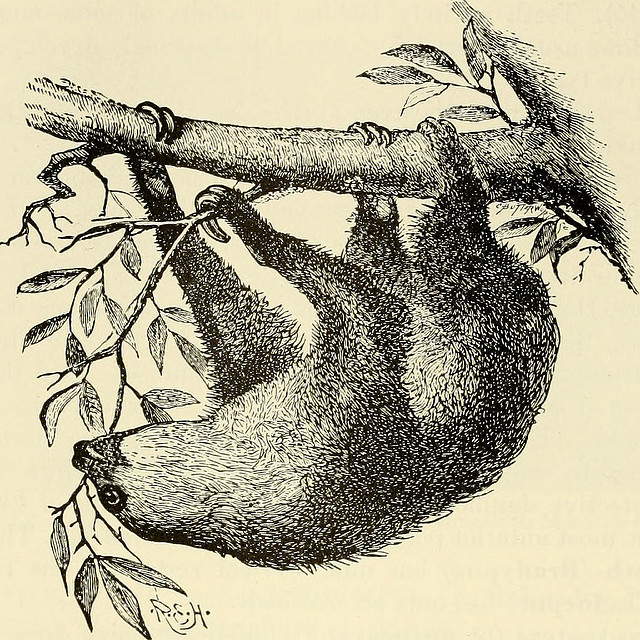
\includegraphics[width=\textwidth]{illustration_images/Genetic_drift/sloth/20423856040_6e4360df9c_z.jpg}
\end{center}
\caption{} \label{fig:sloth}  
\end{marginfigure} 

While most genes evolve under constraint, we can find examples of
genes that are evolving in a less constrained manner. The simplest
example of this is where the gene has lost function, e.g. has recently
become pseudogenized. When a gene completely loses function there will be no
selection against non-synoynous changes and so they are just as free
to accumulate as synonymous changes, and so $\dNdS=1$.
Genes can lose function because of inactivating mutations that stop
them being transcribed or translated into functional proteins, such genes are
called pseudogenes. Our genomes are filled with old pseudogenes whose
meaning are slowly being eroded through the accumulation of neutral substitutions.
One nice example of as gene that has been repeatedly lost function,
i.e. become repeatedly psuedogenized, is
the Enamlin gene from the study of \citeauthor{Meredith:09}.

\begin{figure}
\begin{center}
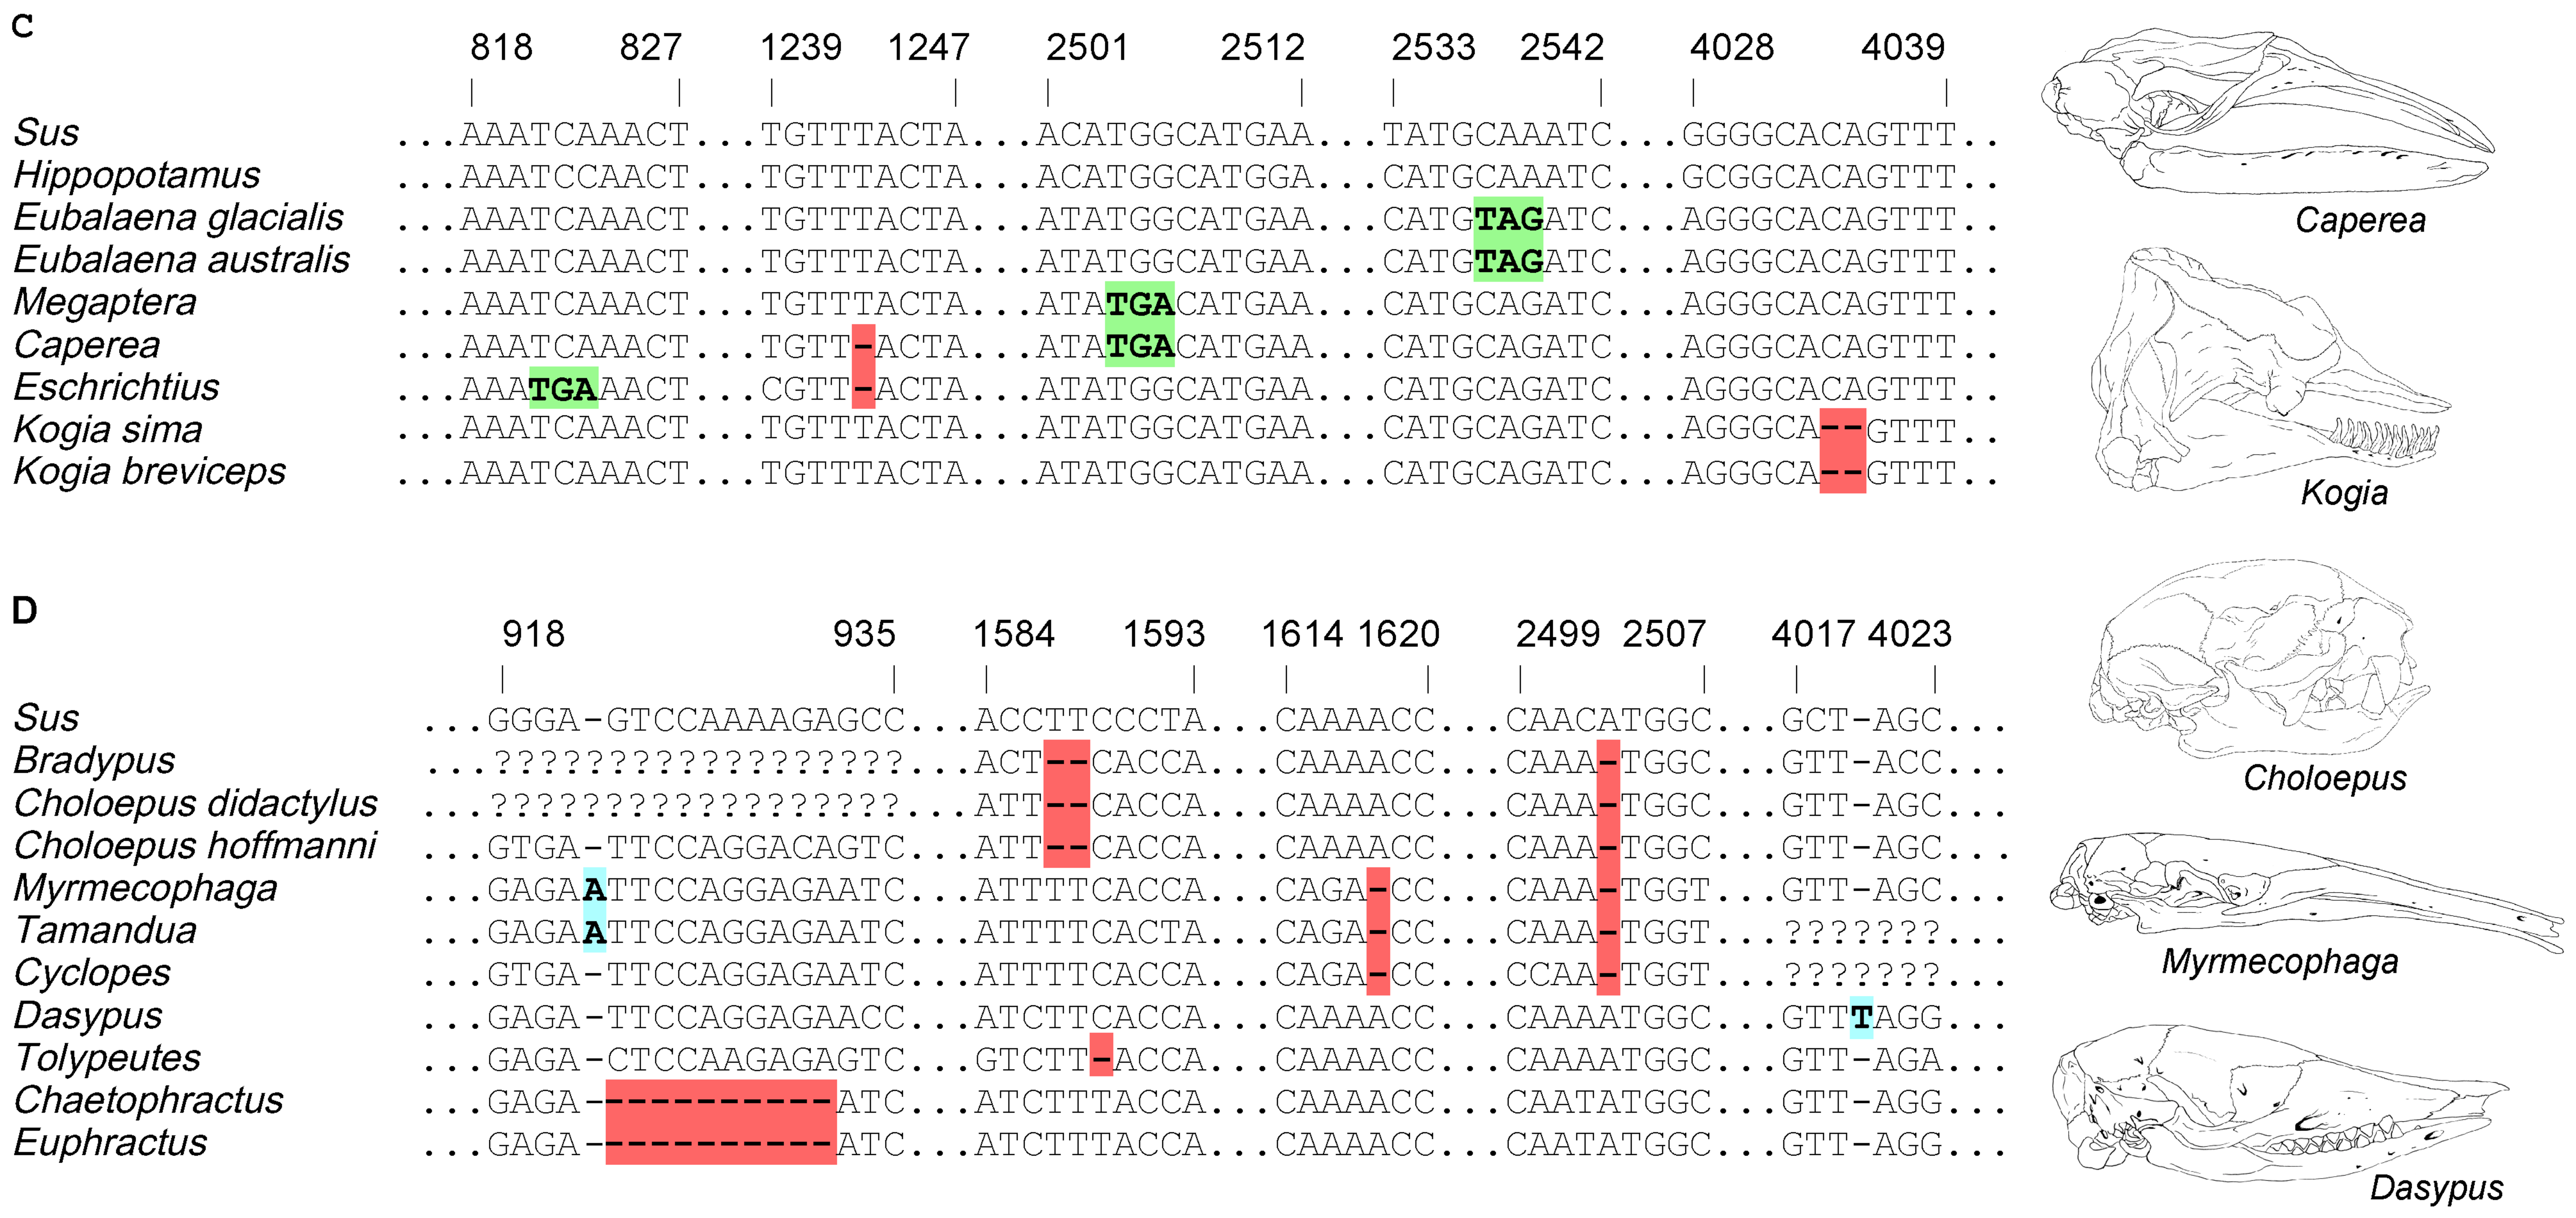
\includegraphics[width=\textwidth]{Journal_figs/genetic_drift/Enamelin/Enamlin.pdf}
\end{center}
\caption{Examples of frameshift mutations (insertions blue, deleteions
  red) and premature stop codons in Enamlin in Cetacea and
  Xenarthra. Figure taken from \citeauthor{Meredith:09}} \label{fig:Enamlin_coding}  
\end{figure} 

\marginnote{
``Rudimentary organs may be compared with the letters in a word, still
retained in the spelling, but become useless in the pronunciation, but
which serve as a clue .. for its derivation.''
}

The protein Enamlin is a key structural protein involved in the outer cap of enamel on teeth. Various mammals have
secondarily evolved to lack enamel on their teeth, because their diet does not
demand hard teeth, e.g. : two-toed sloths ({\it Choloepus}); Pygmy sperm whales ({\it Kogia}); aardvark 
{\it Orycteropus}). While others have lost their teeth entirely: giant anteaters ({\it Myrmecophaga}); Baleen whales, including 
or lack enamel on their teeth.
Due to this loss of selective function
pseudogenizing substitutions, premature stop codons and frameshift mutations, have
accumulated in the gene Enamlin (see Figure \ref{fig:Enamlin_coding}
for examples).  \citeauthor{Meredith:09} sequenced Enamlin across a
range of species and found that none of the species with Enamel have frameshift
mutations in Enamlin, while 17/20 of species that lack Enamel or teeth have
frameshifts in Enamlin and all of them carry premature stop codons
(Figure \ref{fig:Enamlin_phylo}). 

\begin{figure}
\begin{center}
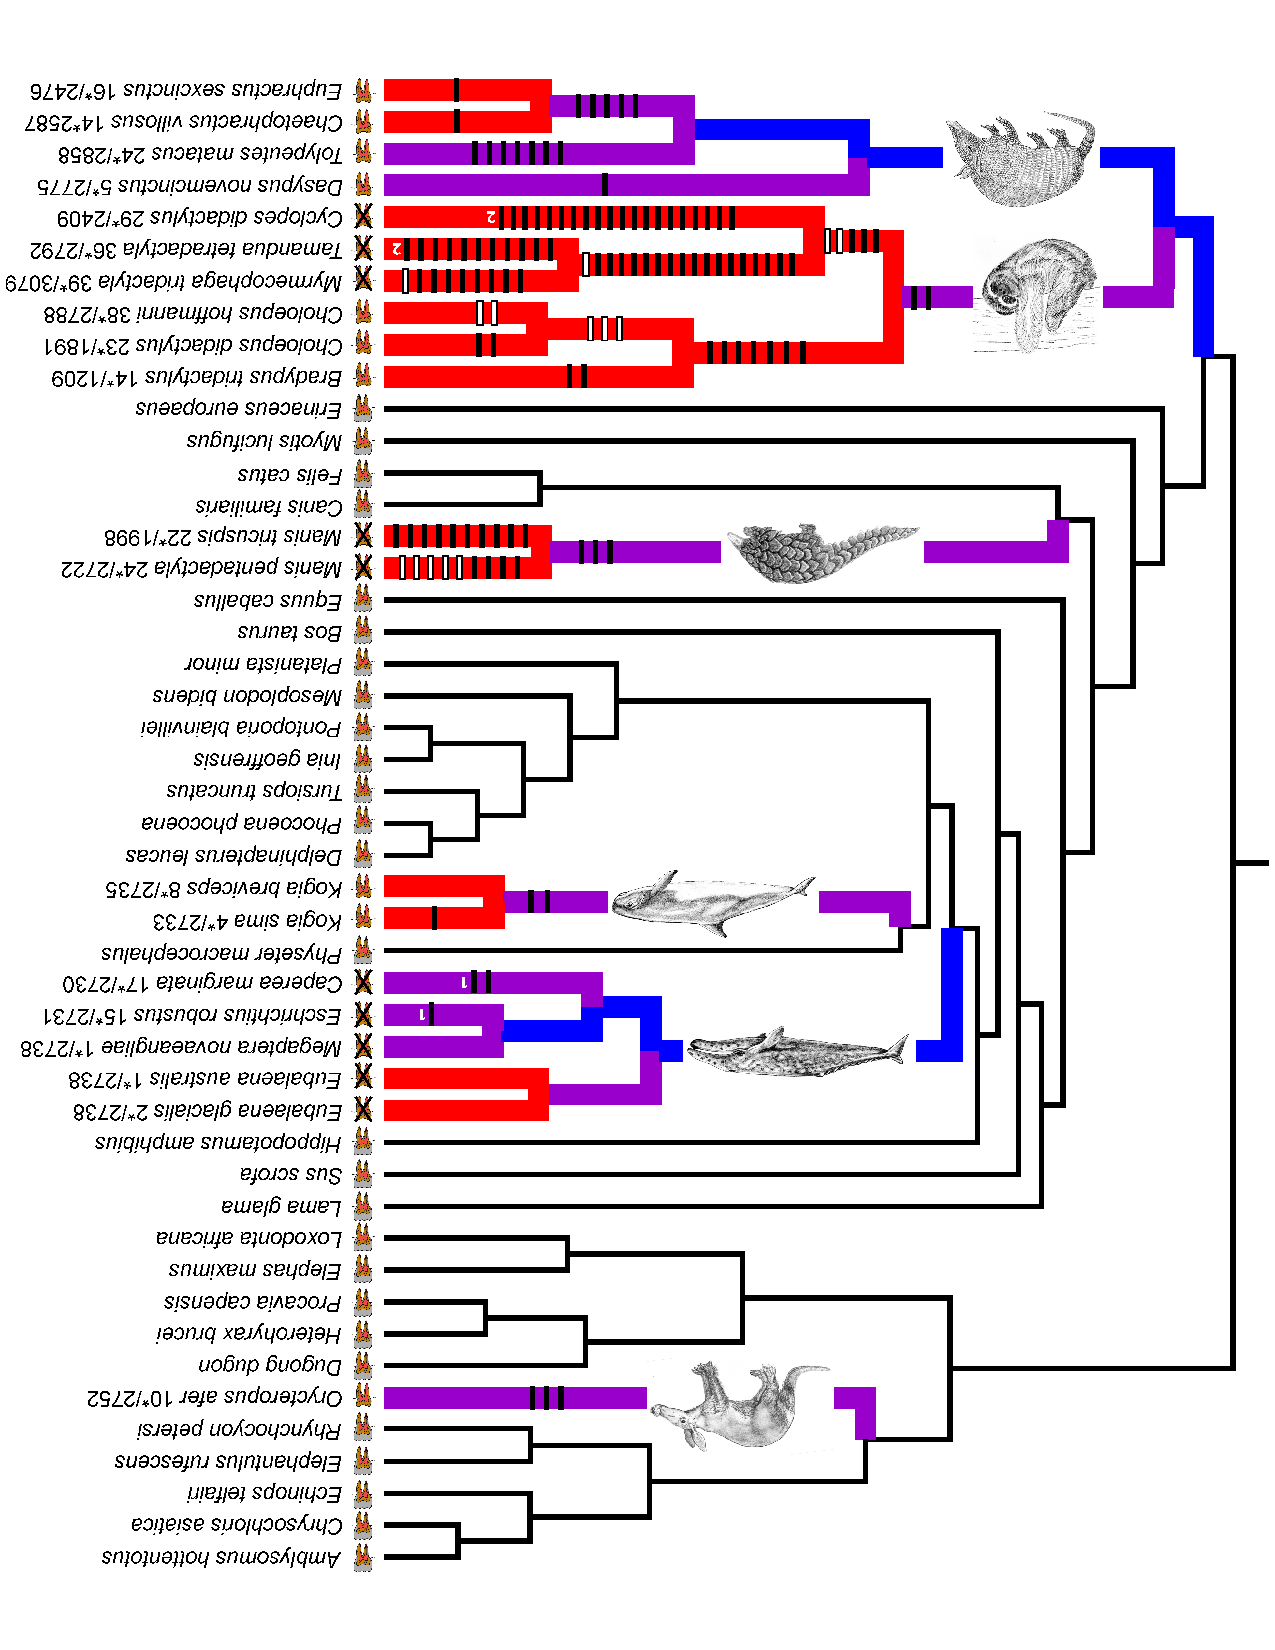
\includegraphics[width=0.8 \textwidth]{Journal_figs/genetic_drift/Enamelin/Enamlin_phylo.pdf}
\end{center}
\caption{The tooth symbol next to each taxon shows whether they have
  teeth, lack enamel, or lack teeth. Branches of the phylogeny are coloured by whether their
  Enamlin is functional (black), pre-mutation (blue), mixed (purple),
  and pseudogenic (red). The black and white vertical bars on branches show frameshift
  mutations.  The Numbers after taxon names indicate minimum number of
  stop codons in the sequence /  the length of the sequence.} \label{fig:Enamlin_phylo}  
\end{figure} 

The branches of the Enamlin phylogeny with a functional Enamlin gene (black)
had an estimated $\dNdS= 0.51$ consistent with the protein evolving in
a constrained manner. While the branches with a pseudogenized Enamlin
had $\dNdS = 1.02$ consistent with the gene evolving an unconstrained
way. The branches where the gene was likely transitioning from a functional
to non-function state (premutation and mixed, blue and purple) had an intermediate values of
$\dNdS=0.83-0.98$ consistent with them transitioning from a
constrained to unconstrained mode of protein evolution.


\paragraph{Adaptive evolution and $\dNdS$.}
Clearly genes are not only subject to neutral and deleterious
mutations, as beneficial mutations must also arise from time to time. 
Lets assume that a fraction $B$ of non-synonymous mutations that arise are
beneficial, and that they fix with probability $f_B$. This fixation
probability may be much higher than that of neutral mutations (we'll
discuss how to calculate the fixation probability for beneficial
alleles in Chapter \ref{Selection_Stochasticity}).  If $T$ generations of divergence have
elapsed between the two populations 
\begin{equation}
2T (1-C - B) \mu  + 2T B f_B \mu
\end{equation}
Then
\begin{equation} 
\dNdS = (1-C-B) +  B f_B
\end{equation}
Note that this means that our estimates of $C$ using $1-\dNdS$ will be
a  lower bound on the true constraint if even a small fraction of
mutations are beneficial.
However, genes may still evolve in a constrained way
(i.e. $\dNdS<1$)  if adaptive substitutions are common at a gene if
they are outweighed by the loss of potential subsitutions to negative selection.

While most genes evolve under constraint, we can find examples of
genes that are evolving in a less constrained manner. The simplest
example of this is where the gene has lost function, e.g. has recently
become pseudogenized. Along branches of the phylogeny where all the
constraint against non-synonymous mutation has
been lost then $\dNdS=1$. We can also identify cases where the gene
is evolving more rapidly at the protein level than at synonymous
sites, i.e. $d_N/d_S > 1$, corresponding to cases of rapid change due
to positive selection. 

\begin{figure}
\begin{center}
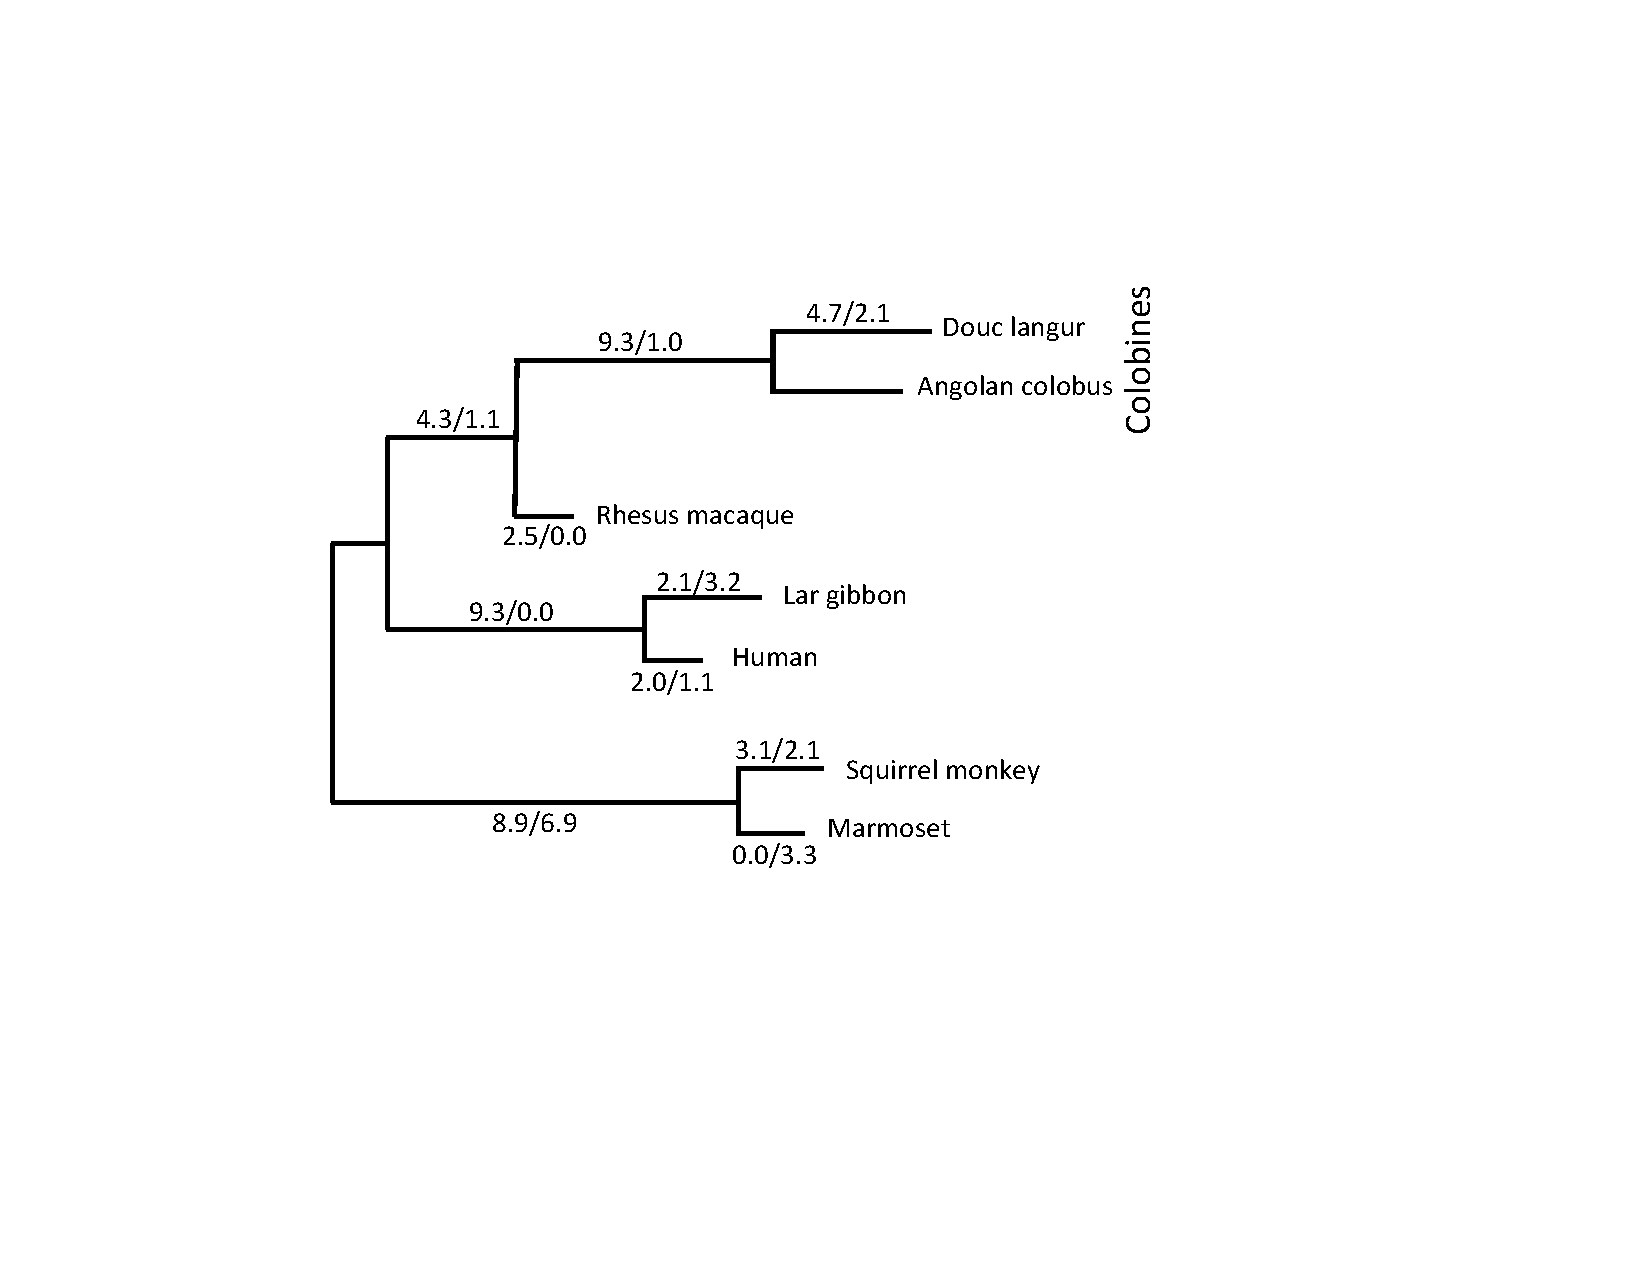
\includegraphics[width=0.8 \textwidth]{Journal_figs/genetic_drift/Yang_lysozyme/Yang_lysozyme.pdf}
\end{center}
\caption{A phylogram for the primate lysozyme gene redrawn from
  \citeauthor{Yang:98}. For each branch the numbers give the estimated average
number of non-synonymous to synonymous changes in the lysozyme protein.} \label{fig:lysozyme}  
\end{figure} 

\begin{marginfigure}
\begin{center}
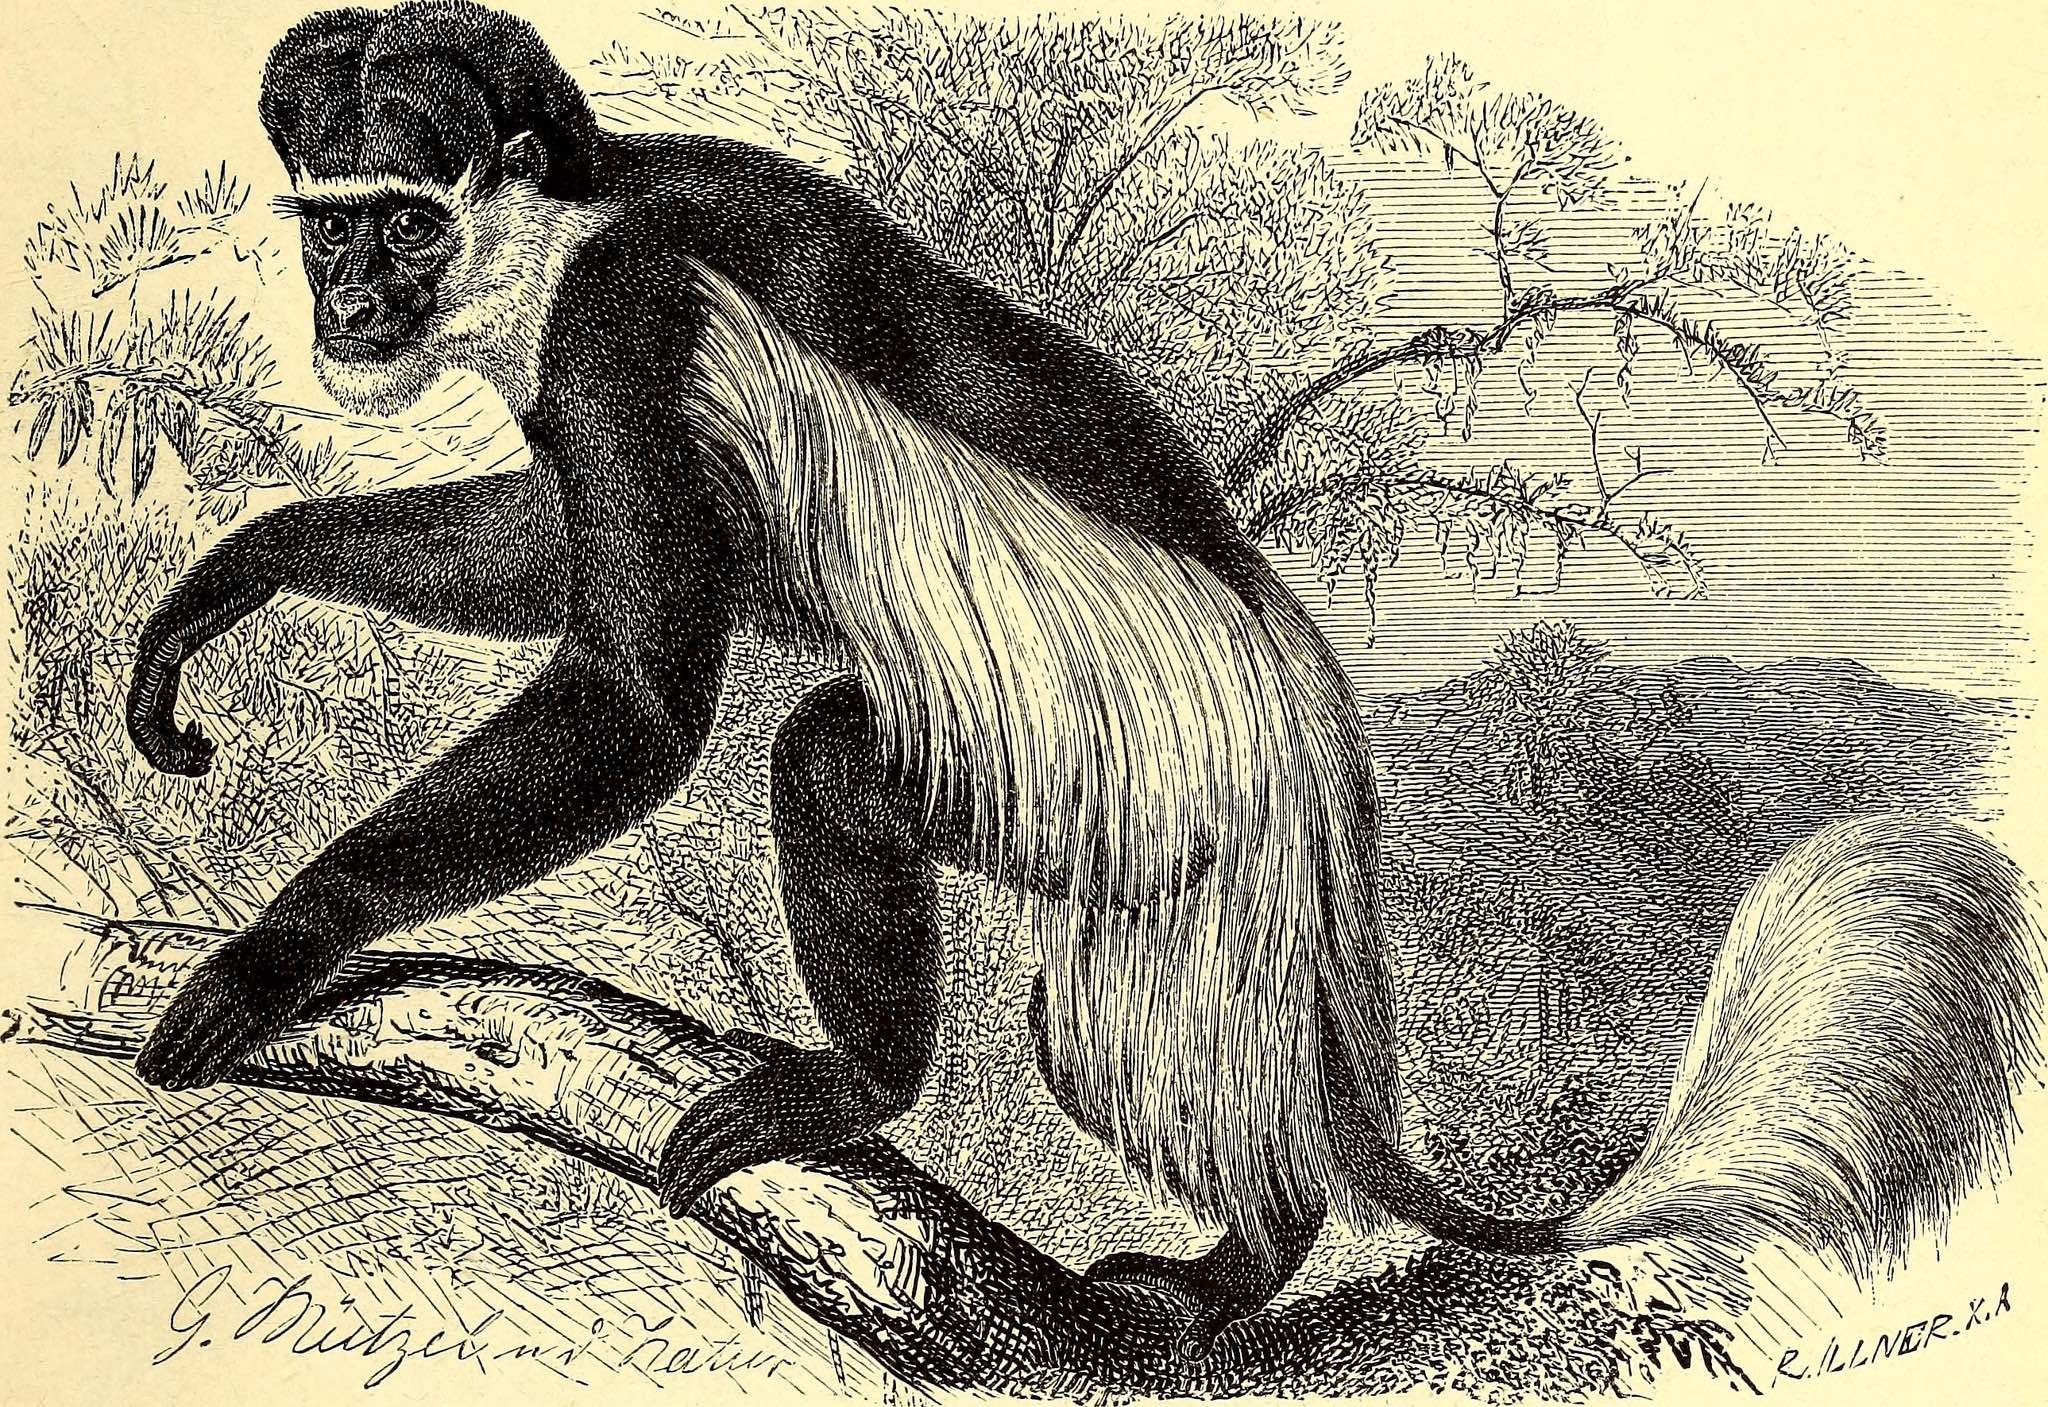
\includegraphics[width=0.8 \textwidth]{illustration_images/Genetic_drift/Colobus/19792029373_fcce706e67_k.jpg}
\end{center}
\caption{Abyssinian black-and-white colobus ({\it Colobus guereza}). Brehm's Tierleben,  Brehm,
  A.E. 1893. A member of the leaf-eating Colobines.} \label{fig:Colobus}  
\end{marginfigure} 

\begin{marginfigure}
\begin{center}
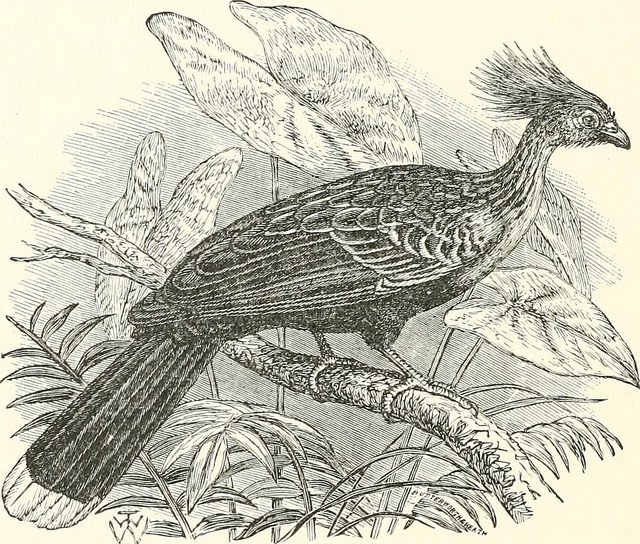
\includegraphics[width=0.8  \textwidth]{illustration_images/Genetic_drift/Hoatzin/14747388314_85798ba97e_z.jpg}
\end{center}
\caption{ (hoatzin ({\it Opisthocomus hoazin}). A history of birds
  Pycraft, W.P. 1910.  A leaf-eating bird.} \label{fig:hoatzin}  
\end{marginfigure} 
A classic example of looking for adaptive evolution using dN/dS is the
evolution of the lysozyme protein in primates \citep{Messier:97,Yang:98}, see
the phylogeny in Figure \ref{fig:lysozyme}. The lysozyme protein is
a key component for the breakdown of bacterial walls. It shows very
fast protein evolution notably on the lineages leading to apes (e.g. gibbons
and humans) and Colobines (e.g. colobus and langur monkeys). Colobines have leaf-based diets. They digest
these leaves by fermentation with bacteria in their foregut, and use lysozymes to break down the bacteria to extract energy from the
leaves. In Colobines the lysozyme protein has evolved to work well in the high-PH environment of the stomach. Remarkably the Colobine
lysozyme has convergently evolved this activity via very similar
amino-acid changes at 5 key residuals as in cows and Hoatzins (a leaf
eating bird). 

\paragraph{The Mcdonald-Kreitman test}
\citet{mcdonald:91} devised a simple test of the neutral theory of molecular
evolution at a gene (building on the conceptually similar HKA
test\cite{HKA}. They partitioned polymorphism and fixed differences into 
nonsynonymous and synonymous changes:
\begin{center}
%\begin{table}
\begin{tabular}{ccc}
 & Poly. & Fixed \\
\hline 
Non-Syn. &    $P_N$  &   $D_N$  \\
Syn. &    $P_S$   &     $D_S$   \\
Ratio & $P_N/P_S$ & $D_N/D_S$
\end{tabular}
\end{center}

Under neutral theory we expect a smaller number of non-synonymous to
synonymous fixed differences ($P_N/P_S < 1$) but exactly the same
expectation holds for polymorphism
($P_N/P_S$). To see this denote the total time on the coalescent genealogy within the species as
$T_{tot}$ and the total time for fixed differences by $T_{div}'$ then:

\begin{marginfigure}
\begin{center}
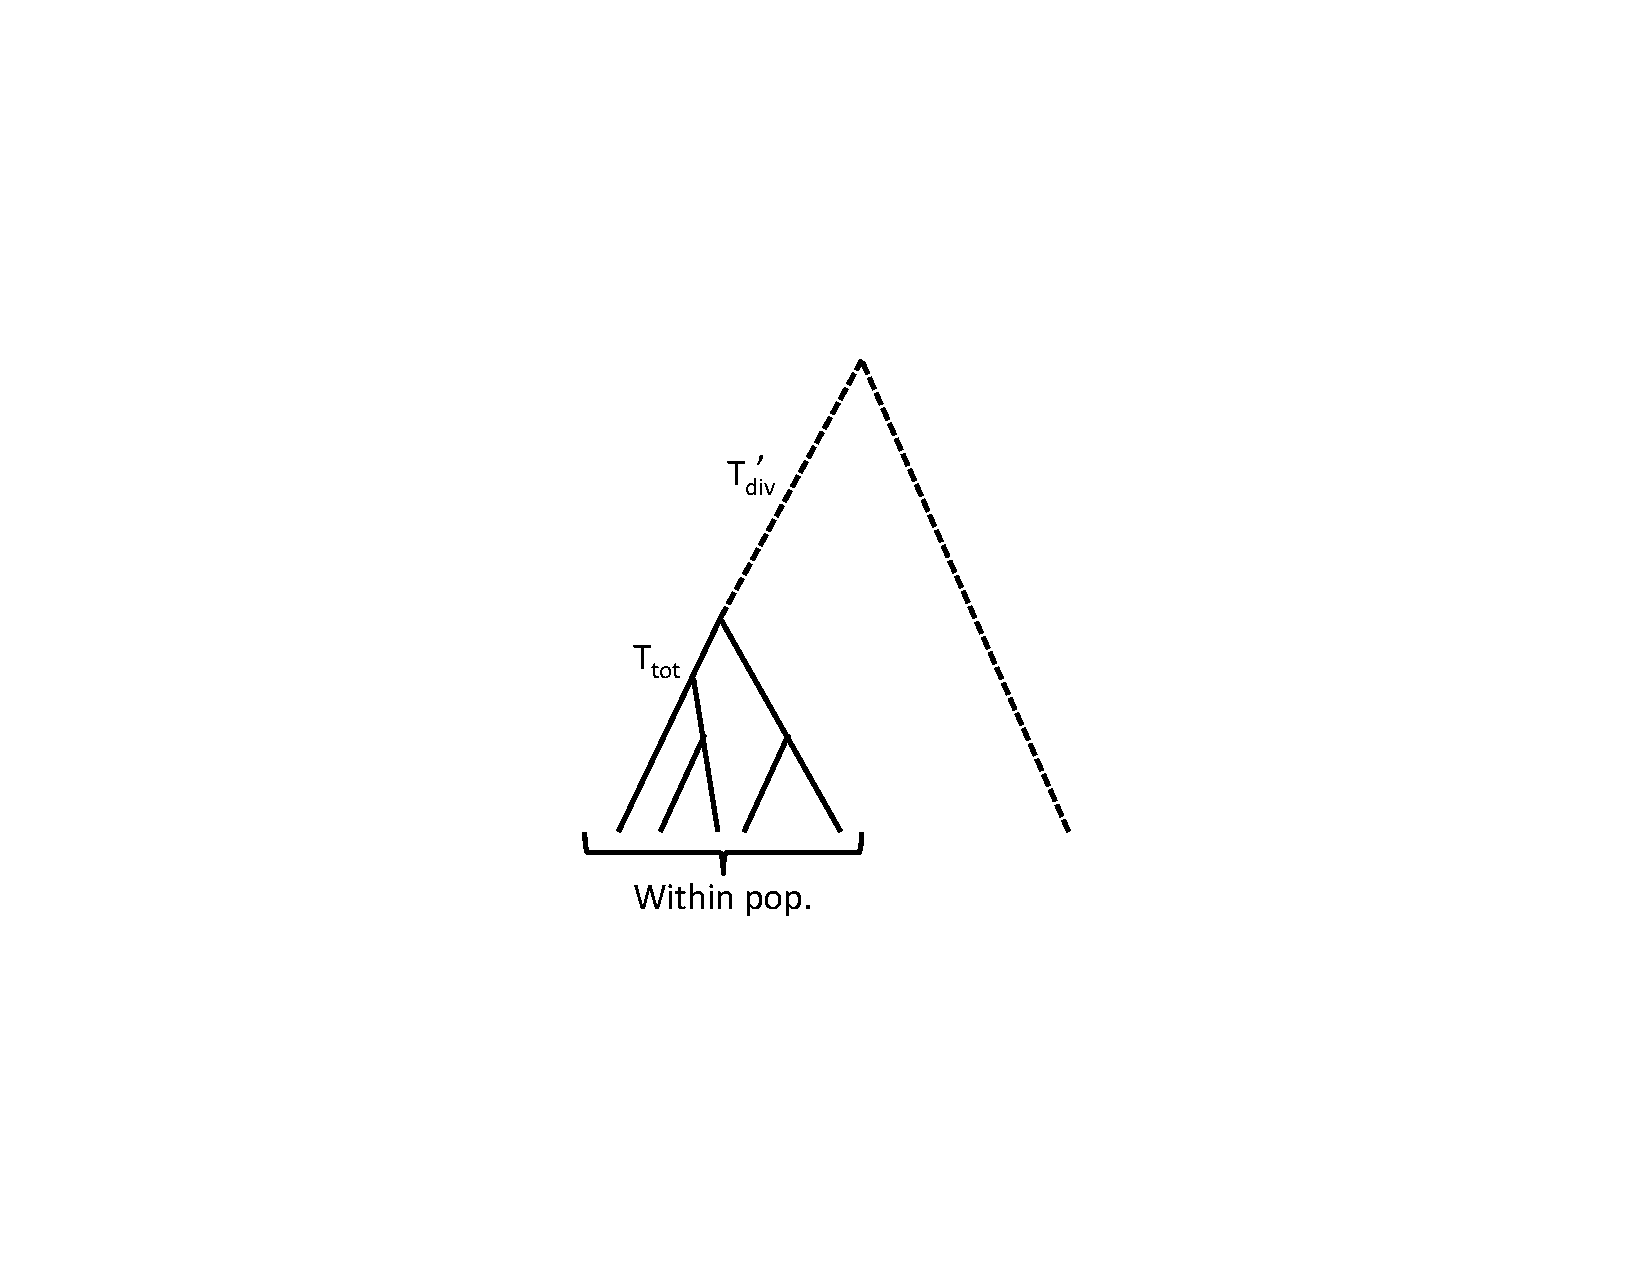
\includegraphics[width=0.8 \textwidth]{figures/Coalescent/MK_tree.pdf}
\end{center}
\caption{ } \label{fig:MK_tree}
\end{marginfigure}

\begin{center}
\begin{tabular}{ccc}
 & Poly. & Fixed  \\
 \hline
Non-Syn. &    $\mu_N T_{tot}$  &   $\mu_N  T_{div}'$ \\
Syn. &    $\mu_S T_{tot}$   &     $\mu_S  T_{div}'$  \\
Ratio & $\mu_N/\mu_S$  & $\mu_N/\mu_S$
\end{tabular}
\end{center}
Therefore, we expect the ratio of non-synonymous to synonymous changes
to be the same for polymorphism and divergence. We can test this expectation of equal ratios via the standard G-test of a $2
\times 2$ table.

\subsection{Neutral diversity and population structure}
%%this section was moved from the coalescent chapter
Up to now we have assumed that our alleles that we have modelled in the
coalescent setting are drawn from a randomly mating population such
that any pair of lineages is equally likely to coalesce with each
other. However, when there is population structure this assumption is
violated. \\

We have previously written the measure of population structure
$\fst$ as
\begin{equation}
\fst = \frac{H_T-H_S}{H_T}
\end{equation}
where $H_S$ is the probability that two alleles sampled at random from a
subpopulation differ, and $H_T$ is the probability that two alleles
sampled at random from the total population differ. 

\paragraph{A simple population split model}
Imagine a population of constant size of $N_e$ diploid individuals that
$\tau$ generations in the past split into two daughter populations (sub-populations)
each of size $N_e$ individuals, who do not subsequently exchange
migrants. In the current day we sample an equal number of alleles
from both subpopulations.

Consider a pair of alleles sampled within one of our
sub-populations, they have experienced a population of size $N_e$
and so the probability that they differ is $H_S = \theta/(1+\theta)$
(where $\theta=4N_e\mu$).
The heterozygosity in our total population is a little more tricky to
calculate. Assuming that we equally sample both sub-populations, when we draw two alleles from our total
sample, $50\%$ of the time they are drawn from the same
subpopulation and $50\%$ of the time they are drawn from different
subpopulations. Therefore, our total heterozygosity is given by
\begin{equation}
H_T = \half H_S + \half H_B
\end{equation}
where $H_B$ is the probability that a pair of alleles drawn from our
two different sub-populations differ from each other. Our pair of
alleles can not find a common ancestor with each other for at least $\tau$
generations into he past as they are in distinct populations (not
connected by migration). The probability that one or other of them
mutates in this time is $1-(1-\mu)^{2T}$. With probability
$(1-\mu)^{2T} $ neither of our alleles mutate in the $T$ generations
back in time before they find themselves back in the combined ancestral 
population. Conditional on failing to mutate before the combined ancestral
population, the probability that they do manage to mutate before
coalescing in that population of size $N_e$ is
$\theta/(\theta+1)$. Putting these components together
\begin{equation}
H_B = \left( 1-(1-\mu)^{2T} \right) + (1-\mu)^{2T}
  \frac{\theta}{\theta+1} 
\end{equation}
We can plug this into our expression for $H_T$, and then that in turn
into $\fst$.

\begin{figure}
\begin{center}
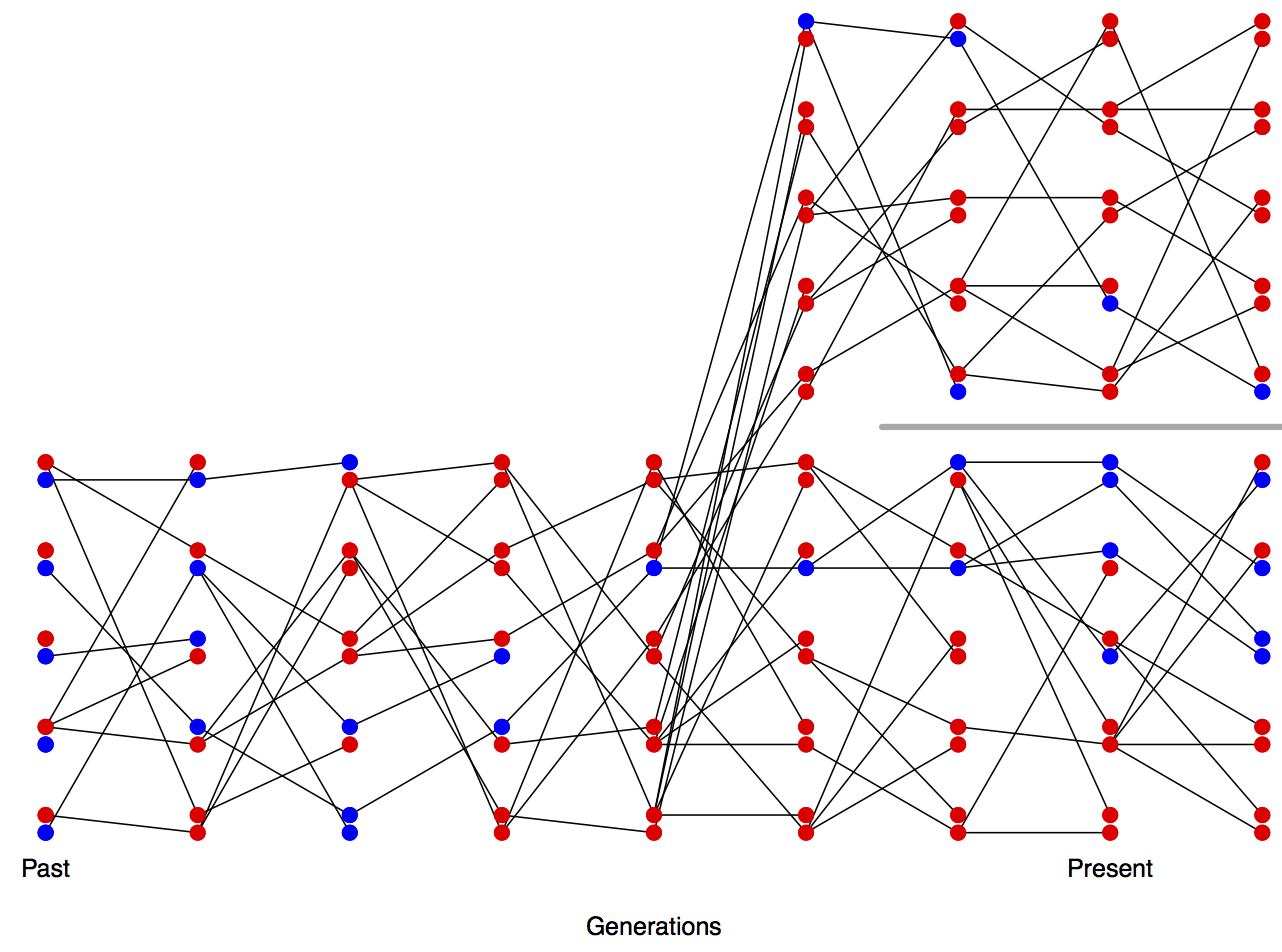
\includegraphics[width= 0.8 \textwidth]{figures/drift_split.png}
\end{center}
\caption{Change in allele frequencies following a population split.} \label{fig:drift_split}  
\end{figure} 

To understand this better we can make a simple
approximation based on our mutation rate being very low, such that
$N_e \mu \ll 1$ so $H_S \approx
4N_e\mu$, and that $\mu \ll 1$ and $\mu T \ll 1$. Assuming this, then  
\begin{equation}
H_B \approx 2 \mu T + 4N_e\mu. 
\end{equation}
So that 
\begin{equation}
\fst \approx \frac{ \mu T}{\mu T +  4N_e\mu }  %= \frac{ T}{ T +  4N_e }
\end{equation}
note that $\mu$ cancels out of this. In this simple toy model $\fst$
is increasing because the amount of between population diversity 
increases with the divergence time of the two populations (initially
linearly with $T$). It does so at a rate
give by $\nicefrac{T}{(4N_e)}$ so that differentiation will be higher
between populations separated by long divergence times or with small
effective population sizes.

\begin{question}
The gorilla lineage split from the human-chimp lineage $\sim$7 million years ago. Let’s assume that this speciation event occurred instantaneously in allopatry with no subsequent gene flow. \\
{\bf A)}	What is the probability of that gorilla is not an outgroup to human and chimp at a single locus?\\
{\bf B)}	It has been estimated that the gorilla lineage is not an outgroup at around ~30\% of autosomal loci. What effective population size would you need to assume to explain this observation? Is that only plausible explanation?\\
{\bf C)}	The gorilla lineage is an outgroup for large portions of the X chromosome, what is a plausible explanation for this finding?
\end{question}

\paragraph{A simple model of migration between an island and the mainland.}
We can also use the coalescent to think about patterns of
differentiation under a simple model of migration drift
equilibrium. Lets consider a small island population that is relatively isolated
from a large mainland population, and that both of these populations
are constant in size. We'll assume that the expected heterozygosity
for a pair of alleles sampled on the mainland is $H_M$.

Our island has a population size
$N_{I}$ that is very small compared to our mainland population.
Each generation some low fraction $m$ of our individuals on the
island have migrant parents from the mainland the generation
before. Our island may also send migrants back to the mainland, but
these are a drop in the ocean compared to the large population size on
the mainland and their effect can be ignored. 


If we sample an allele on the island back and trace its ancestral
lineage backward in time, each generation our ancestral allele have a low
probability $m$ of being descended from the mainland in the proceeding
generation (if we go far enough the allele eventually has to be
descended from an allele on the mainland). The probability that a pair of alleles sampled on the
island are descended from a shared recent common ancestral allele on the island, is the
probability that our pair of alleles coalesce before either lineage
migrates. For example, the probability that our pair of alleles
coalesce $t+1$ generations back is 
\begin{equation}
\frac{1}{2N_I}(1-m)^{2(t+1)} \left(1-\frac{1}{2N_I} \right)^{t} \approx
\frac{1}{2N_I} \exp\left( -t\left (\frac{1}{2N_I} + 2m\right) \right),
\end{equation}
with the approximation following from assuming that $m \ll 1$ \& $\frac{1}{(2N_I)}
\ll 1$ (note that this is very similar to our derivation of
heterozygosity above). The probability that our alleles coalescence before either one
of them migrates off the island, irrespective of the time, is
\begin{equation}
\int_0^{\infty} \frac{1}{2N_I} \exp\left( -t\left (\frac{1}{2N_I} +
2m\right) \right) dt = \frac{\nicefrac{1}{(2N_I)}}{\nicefrac{1}{(2N_I)} +
    2m}.
\end{equation}

Lets assume that the mutation rate is very low such as it is very
unlikely that the pair of alleles mutate before they coalesce on the
island. Therefore, the only way that the alleles can be different from
each other is if one or other of them migrates to the mainland, which
happens with probability  
\begin{equation}
  1 - \frac{\nicefrac{1}{(2N_I)}}{\nicefrac{1}{(2N_I)} + 2m}
\end{equation}
Conditional on one or other of our alleles migrating to the mainland,
both of our alleles represent independent draws from the mainland and
so differ from each other with probability $H_M$. Therefore, the level of
heterozygosity on the island is given by
\begin{equation}
  H_I = (1 - \frac{\nicefrac{1}{(2N_I)}}{1/(2N_I) + 2m})H_M
\end{equation}
So the reduction of heterozygosity on the island compared to the
mainland is
\begin{equation}
  F_{IM} = 1- \frac{H_I}{H_M} = \frac{\nicefrac{ 1}{(2N_I)}}{\nicefrac{1}{(2N_I)} + 2m} = \frac{ 1 }{1 + 4N_Im}.
\end{equation}
The level of inbreeding on the island compared to the mainland will
be high in the migration rate is low and the effective population size
of the island is low, as allele frequencies on the island are drifting
and diversity is not being replenished on the island by migration. The
key parameter here is the number individuals on the island replaced by
immigrants from the mainland each generation ($N_I m$).

We have framed this as being about the reduction in genetic diversity on the
island compared to the mainland. However, if we consider collecting 
individuals on the island and mainland in proportion to population
sizes the total level of heterozygosity would be $H_T=H_M$, as samples
from our mainland would greatly outnumber those from our
island. Therefore, considering our island our sub-population we have
derived another simple model of $F_{ST}$.

\begin{question}
You are investigating a small river population of sticklebacks, which receives infrequent migrants from a very large marine population. At a set of (putatively neutral biallelic markers the freshwater population has frequencies:\\
0.2, 0.7, 0.8\\
at the same markers the marine population has frequencies:\\
0.4, 0.5 and 0.7.\\
 From studying patterns of heterozygosity at a large collection of markers, you have estimated the long term effective size of your freshwater population is 2000 individuals.\\
What is your estimate of the migration rate from the marine
populations into the river?
\end{question}

\paragraph{Incomplete lineage sorting}

Because it can take a long time for an polymorphism to drift up or down in
frequncy, multiple population splits may occur during the transit of
an allele. This can lead to incongruence between the overall
population tree  and the information about relationships present at
individual loci. In Figure \ref{fig:NoILS_poly} and \ref{fig:ILS_poly}
we show a simulations
of three populations where the bottom population splits off from the
other two first, followed by the subsequent spliting of the the top
and the middle population. We start both simulations with a newly
introduced red allele being polymorphic in the combined ancestral
polymorphism. The most likely fate of this allele is that it is
quickly lost from the population, but sometimes the allele can drift
up in frequency and be polymorphic when the populations split, as the
alleles in our two figures have done. If the allele is lost/fixed in
the descendent populations before the next population split our allele
configuration will agree with the population tree, as it does in
Figure  \ref{fig:NoILS_poly}. However, if the allele persists as a
polymorphism in the ancestral population till the top and the middle
populations split, then the allele can fix in one of these populations
and not the other. Such an event can lead to a substitution pattern
that disagrees with the population tree, as in \ref{fig:ILS_poly}.  If
we were construct a phylogeny using the variation we would see a
disagreement between the gene tree and species tree.

\begin{figure}
\begin{center}
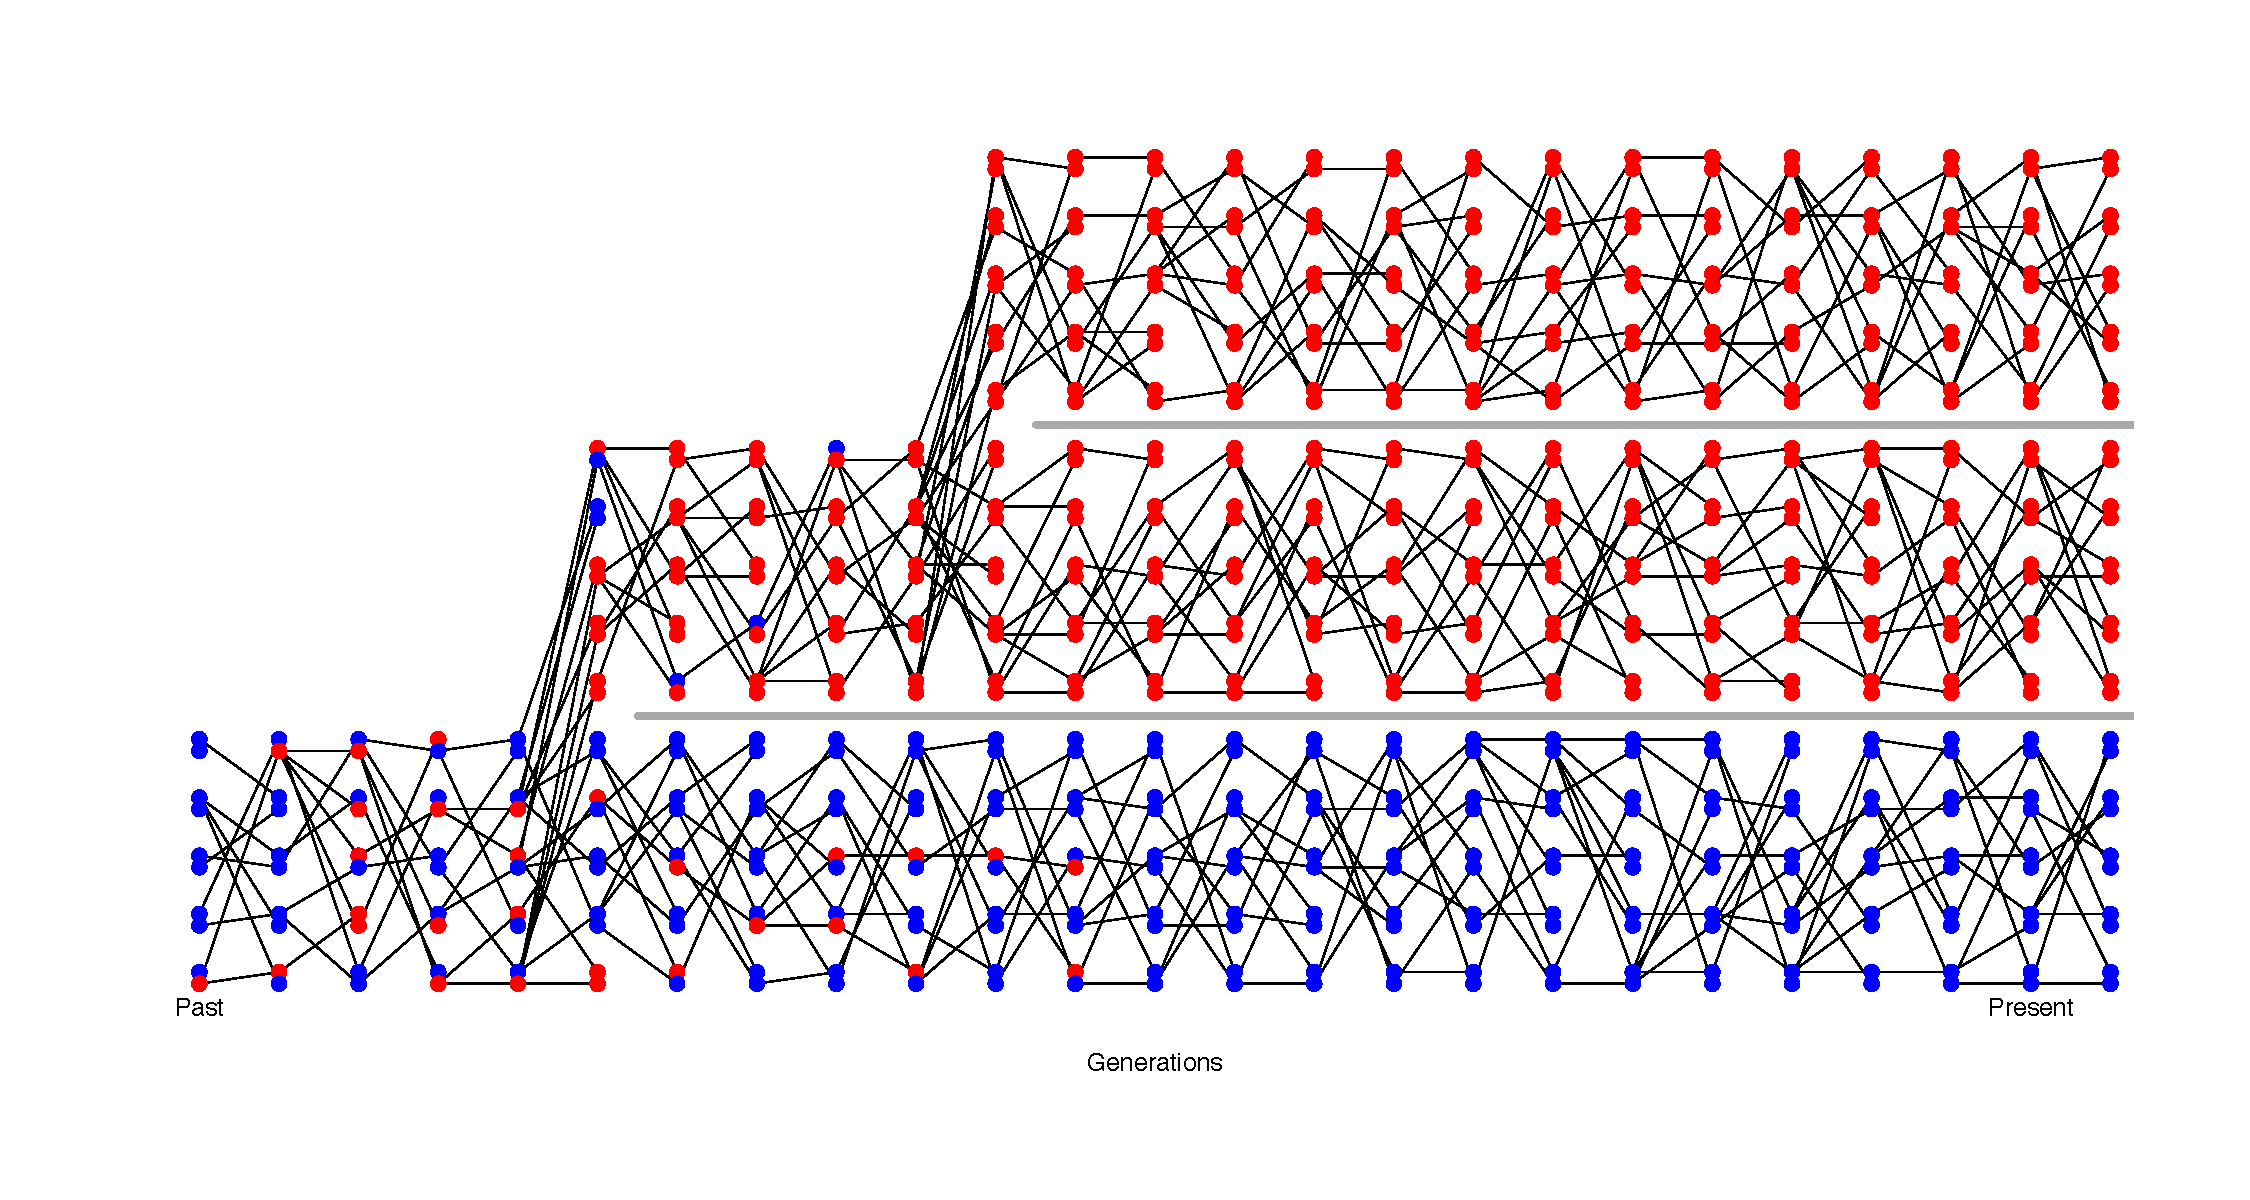
\includegraphics[width=\textwidth]{figures/Genetic_drift/ILS/no_ILS.pdf}
\end{center}
\caption{  } \label{fig:NoILS_poly} 
\end{figure}

\begin{figure}
\begin{center}
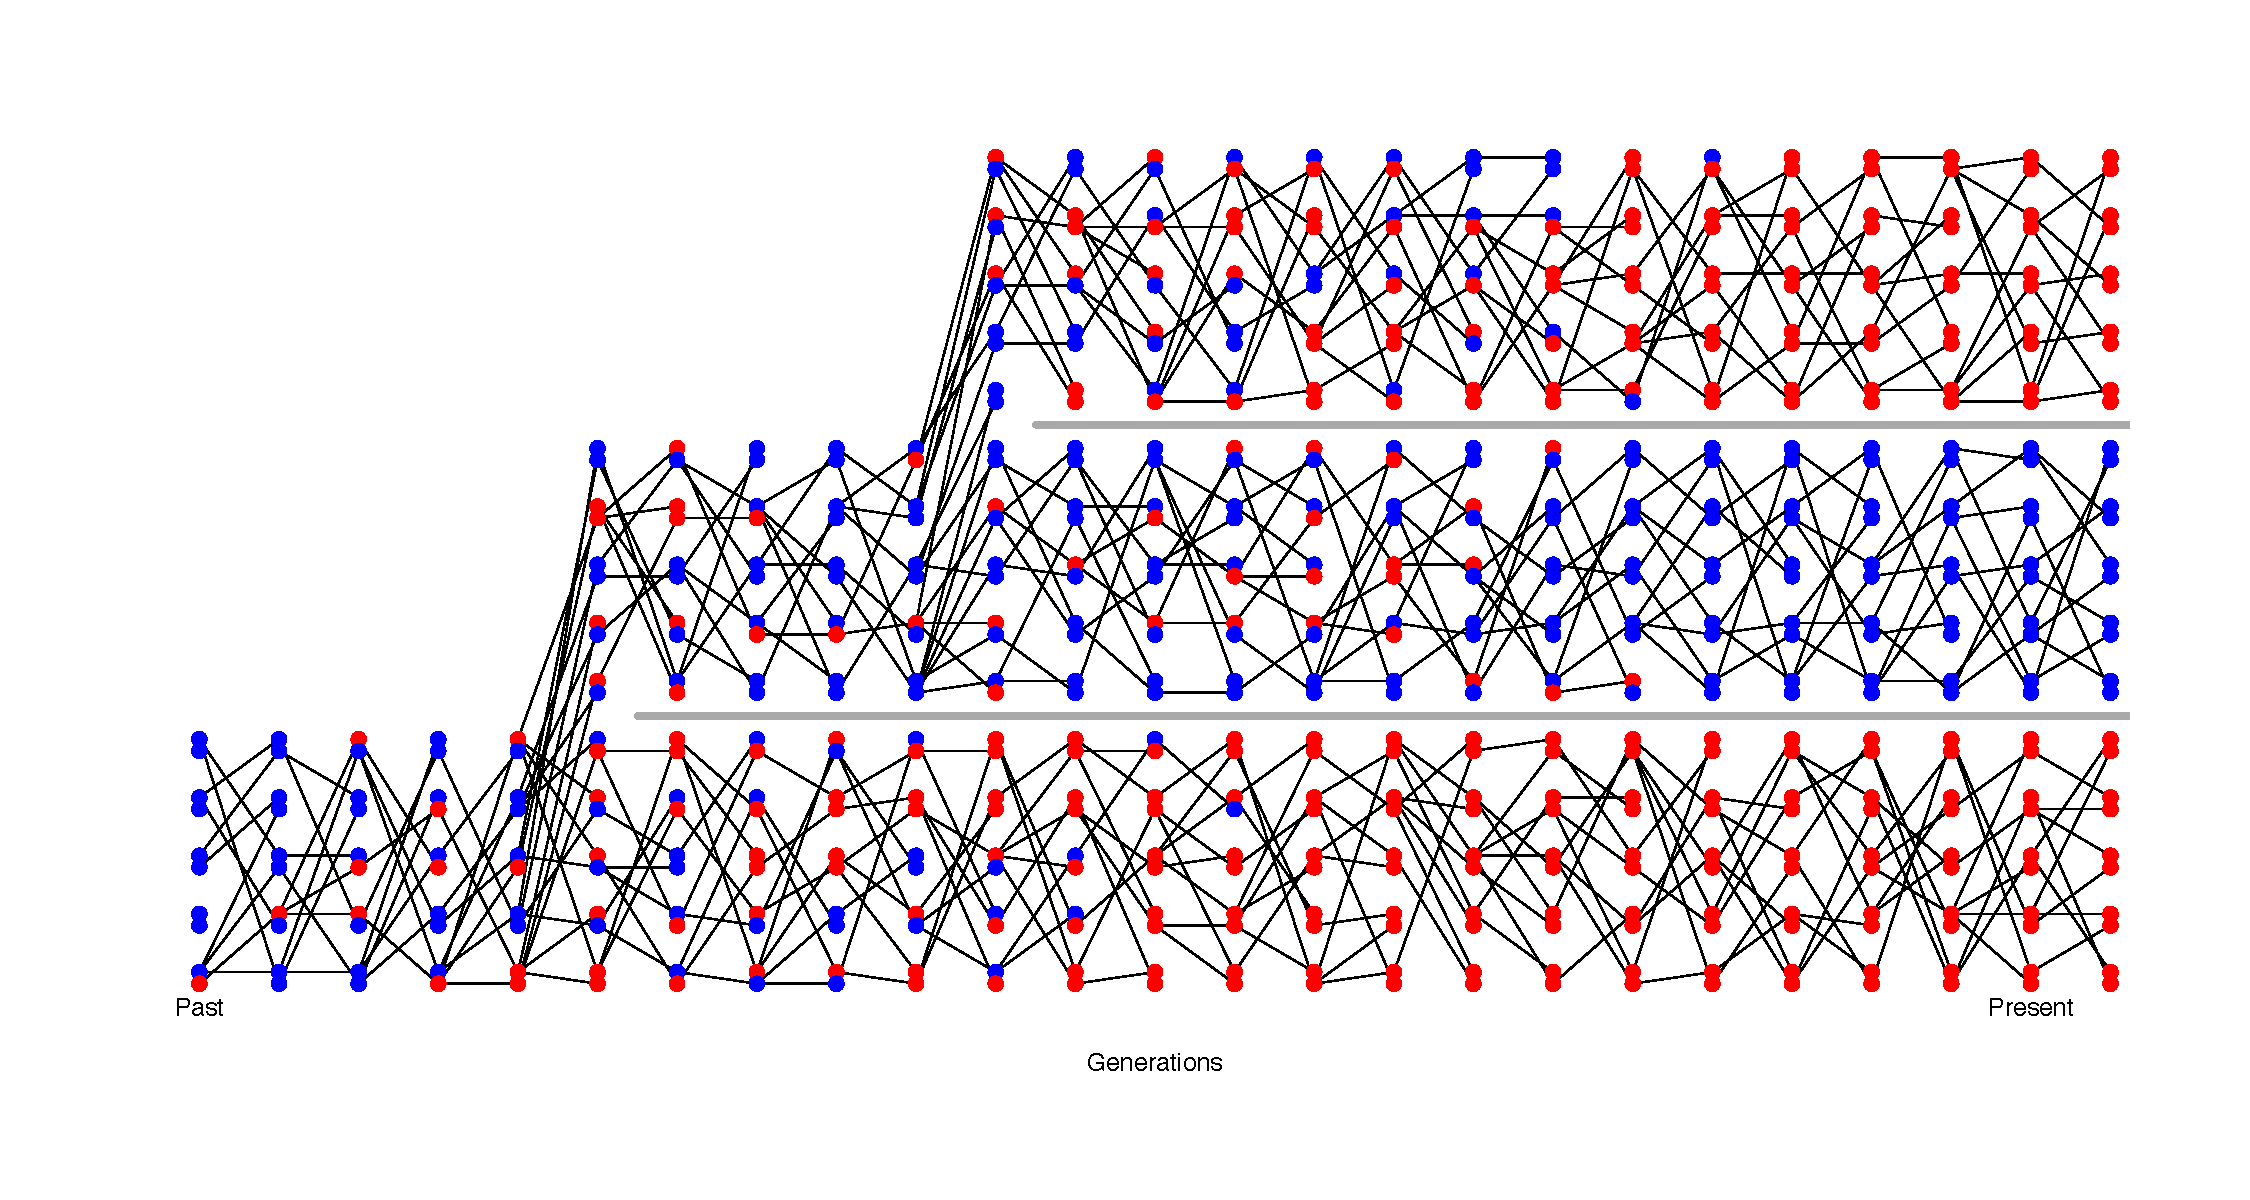
\includegraphics[width=\textwidth]{figures/Genetic_drift/ILS/ILS.pdf}
\end{center}
\caption{  } \label{fig:ILS_poly} 
\end{figure}

A natural, pedigree analogy to this is the fact that while two
biological siblings are morely closely related to each other than
either is to their cousin, at any given locus one of the siblings can
shared an allele IBD with their cousin that they do not share with
their own sibling, due to the randomness of mendelian segregating down their
pedigree. The average relatedness of the individuals/population disagrees
with the patterns of relatedness at a particular locus.

\begin{marginfigure}
\begin{center}
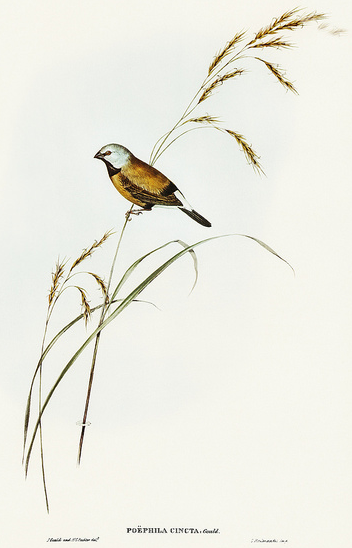
\includegraphics[width=\textwidth]{illustration_images/Genetic_drift/Poephila_cincta_finch/Poephila_cincta_finch.png}
\end{center}
\caption{Banded Grass Finch ({\it P. cincta}). Illustration by
  Elizabeth Gould. Birds of Australia Gould J. 1840. } \label{fig:Poephila_cincta} 
\end{marginfigure}

\citeauthor{jennings:05} sequenced a single allele from three
different species of Australian grass finches (Poephila); two sister species
of long-tailed finches ({\it Poephila acuticauda} and {\it P. hecki})
and the black-throated finch ({\it Poephila cincta}, see Figure \ref{fig:Poephila_cincta}). They collected
sequence data for 30 genes, and constructed phylogenetic gene trees
at each of these loci, resulting in 28 well resolved gene trees. 
16 gene trees of the gene trees showed {\it
  P. acuticauda} and {\it P. hecki} as sisters with {\it P. cincta})
(the tree ((A,H),C)~). While for twelve genes the gene tree was
discordant with the population tree: for seven of their genes  {\it P. hecki}
fell as an outgroup to the other two; and at five {\it P. acuticauda} fell as an outgroup (the trees ((A,C),H) and
((H,C),A) respectively). 

\begin{figure}
\begin{center}
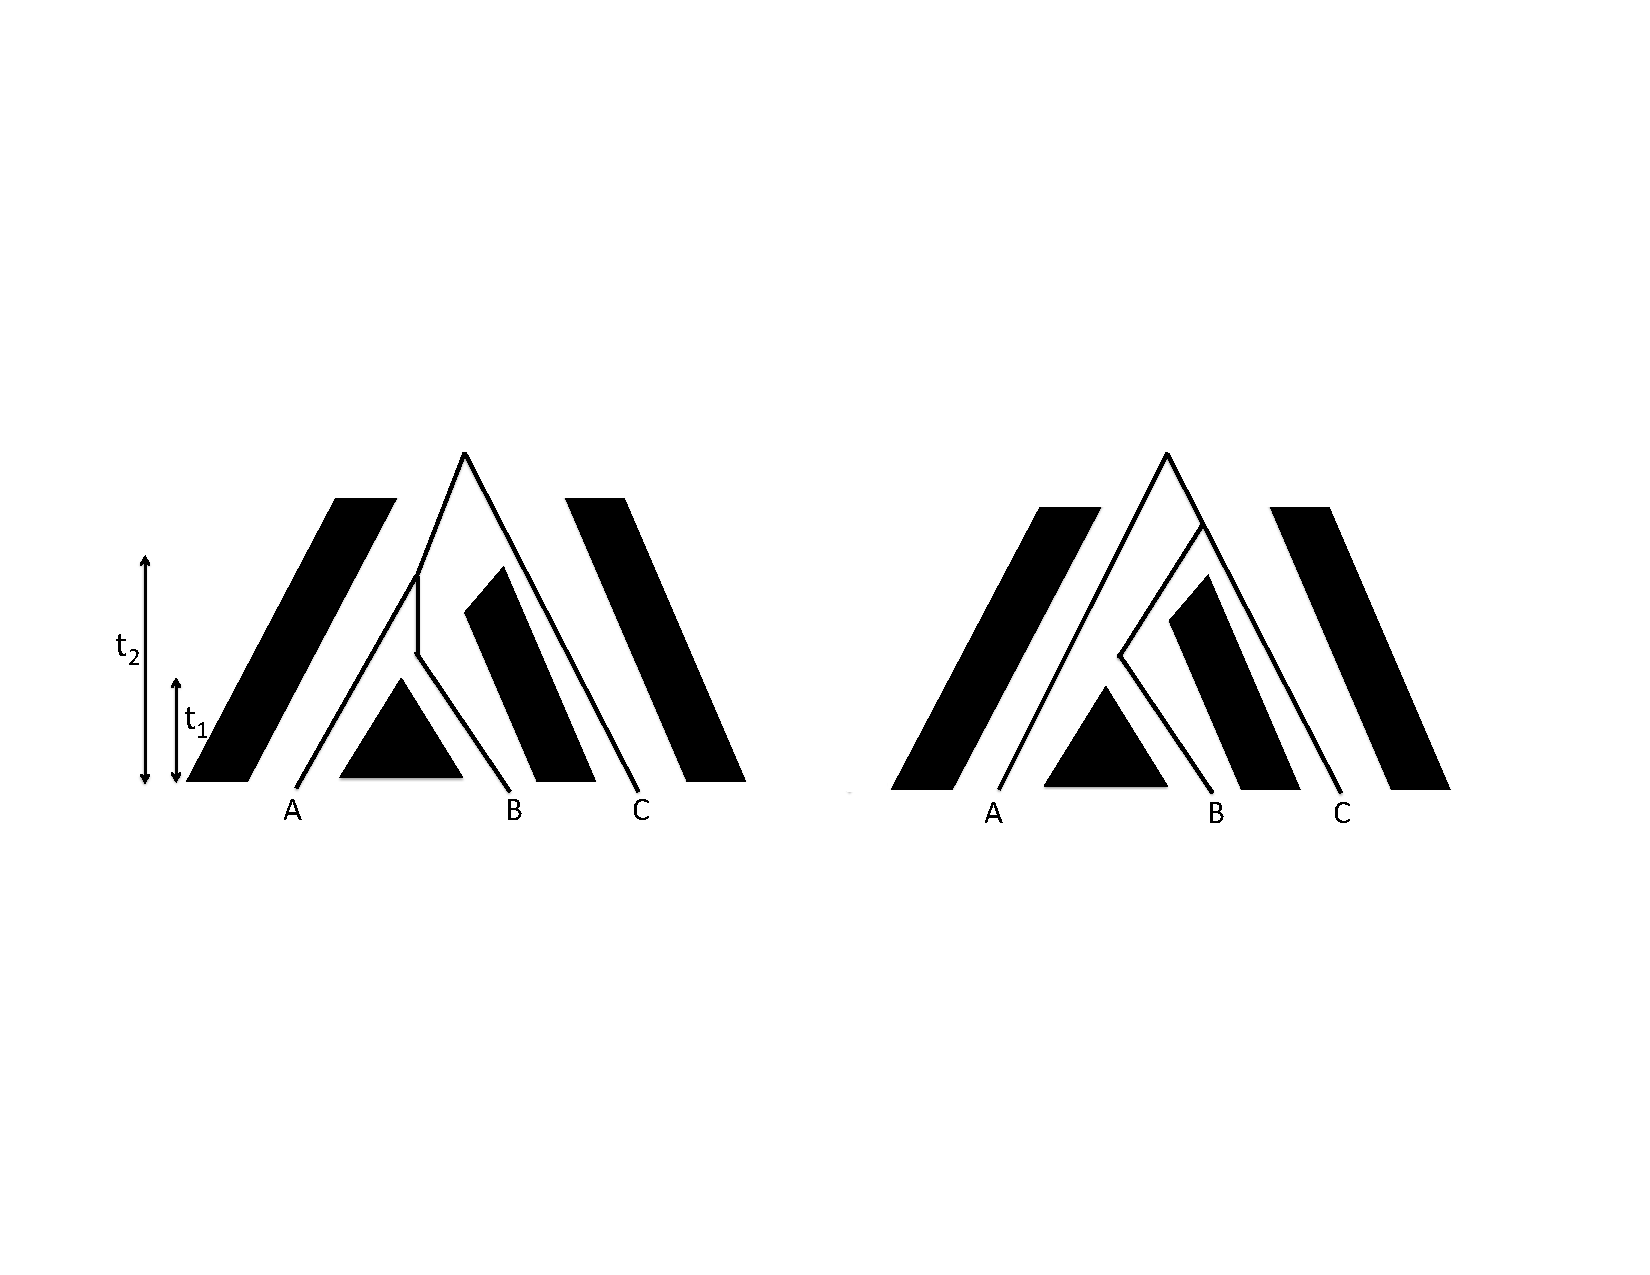
\includegraphics[width=\textwidth]{figures/Genetic_drift/ILS/ILS_coal_cartoon.pdf}
\end{center}
\caption{The population tree of three populations ((A, B), C) is shown
blocked out with black shapes. Two different coalescent trees are
relating a single allele drawn from A, B, and C are shown with thinner lines.} \label{fig:ILS_cartoon} 
\end{figure}
Lets use the coalescent to understand this discordance between gene
trees and species trees. Lets assume that two sister populations
(A \& B) split $t_1$ generations in the past, with a
deeper split from a third outgroup population (C) $t_2$ generations in the
past. We'll assume that there's no gene flow among our populations
after each split. We can trace back the ancestral lineages of our three alleles. The
first opportunity for the A \& B lineages to coalesce is $t_1$
generations. If they coalesce with each other in their shared
ancestral population before $t_2$ in the past, left side of
\ref{fig:ILS_cartoon}, their gene tree will
definitely agree with the population tree. So the only way for the gene
tree to disagree with the population tree is for the A \& B lineages
to fail to coalesce in their shared ancestral population, this happens
with probability $\left(1 - \nicefrac{1}{2N}\right)^{t_2-t_1}$. We'll
get a discordant gene tree, if A
\& B make it back to the shared ancestral population with C without
coalescing, and then one or other of them coalesces with the C
lineage first. This happens with probability $2/3$, as at the first
pairwise-coalescent event there are are three possible pairs two of
which (A \& C  and B \$ C ) result in a discordant tree. So the
probability that we get a coalescent tree that is discordant with the
population tree is
\begin{equation}
\frac{2}{3} \left(1 - \nicefrac{1}{2N}\right)^{t_2-t_1}.
\end{equation}
Thus we should expect gene-tree population-tree discordance when
population split in rapid succession, and/or population sizes are
large. 
\begin{question}
Lets return to \citeauthor{jennings:05}'s Australian grass finches
example, they estimated that the ancestral population size of our two
long-tailed finches was four hundred thousand. What is your best
estimate of the inter-speciation time, i.e. $t_2-t_1$? 
\end{question}

\paragraph{Testing for gene flow.} 

We often want to test whether gene flow has occurred between populations. For example, we might want to establish a case
that interbreeding between humans and Neanderthals occurred or demonstrate that
gene flow occurred after two populations began to speciate. 
A broad range of methods have been designed to test for gene flow, and
toestimate gene flow rates, based on neutral expectations. Here'll we
briefly just discuss one method based on
some simple coalescent ideas.  Above we assumed that gene-tree population-tree discordance was due to
incomplete lineage sorting due to populations rapidly
spliting. However, gene flow among populations can also lead to gene-tree discordance.
While both ILS and gene flow can lead to discordance, under
simplifying assumptions ILS implies more symmetry in how these
discordancies manifest themselves.\\


\begin{figure}
\begin{center}
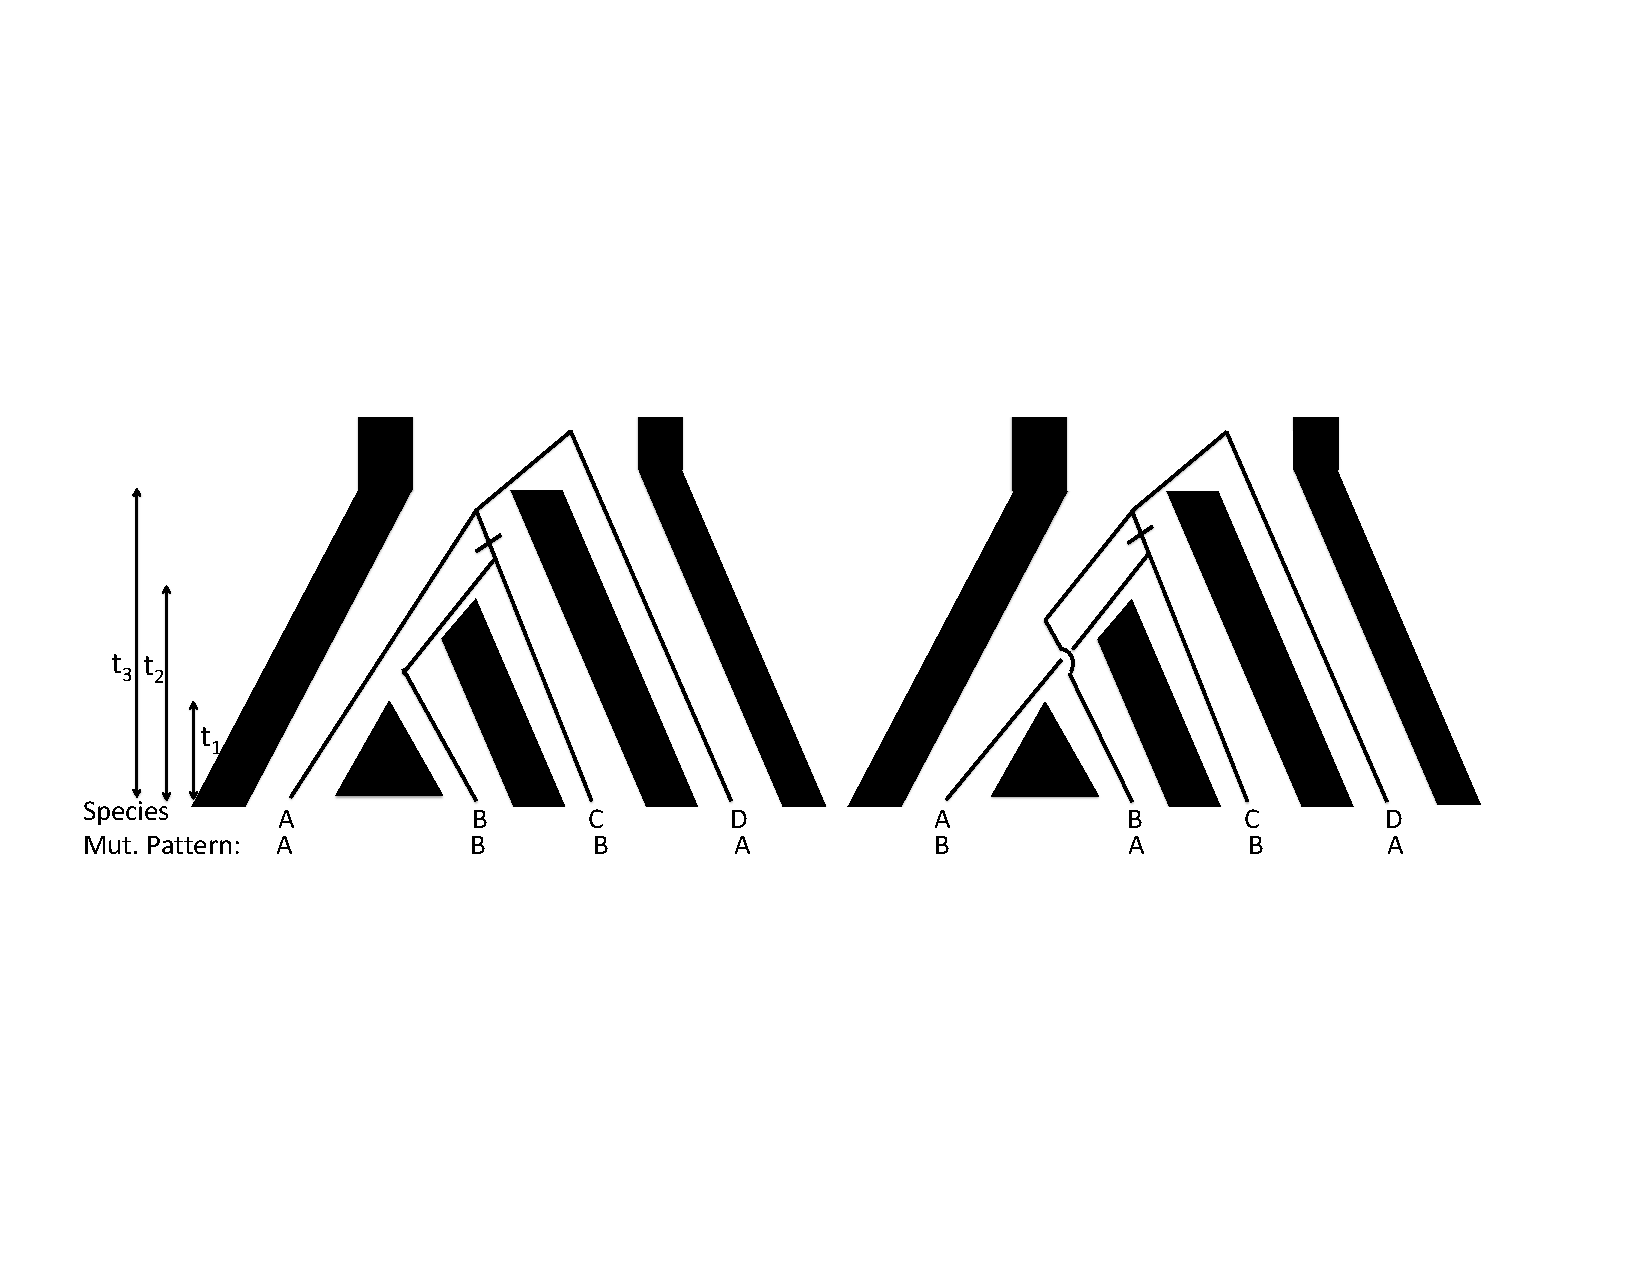
\includegraphics[width=\textwidth]{figures/Genetic_drift/ILS/ABBA_BABA_coal.pdf}
\end{center}
\caption{ In boh the left and and right trees ILS has occurred between our single lineages sampled from populations A, B, and C. Imagine that population D, is an somewhat distant outgroup
such that the lineages from A-C (nearly) always coalesce with each
other, before coalescing with D. The small dash on the branch
indicates the mutation A$\rightarrow$B occuring, giving rise to the
mutational patter shown at the bottom. } \label{fig:ABBA_BABA} 
\end{figure}

Take a look at Figure \ref{fig:ABBA_BABA}. \graham{switch to
  1-4?}. In both cases the lineages from A and B fail to coalesce in
their initial shared ancestral population, and one or other of them
coalesces with the lineage from C first. Each option is equally
likely, therefore the mutational patterns ABBA and BABA are equally
likely to occur under ILS.  \sidenote{here we have to assume no
  structure in the ancestral population.}

However, if gene flow occurs from population C into population B the
lineage from B can more recently coalesce with lineage C, and so we
should see more ABBAs than BABAs. To test for this we can sample four
sequences from our populations and count up the number of sites that
show the two mutational patterns consistent with the gene-tree discordance $n_{ABBA}$ and
$n_{BABA}$ and take 
\begin{equation}
\frac{n_{ABBA}-n_{BABA}}{n_{ABBA}+n_{BABA}}
\end{equation}
this statistic will have expectation zero if the gene-tree discordance
is due to ILS, and be skewed negative if gene flow
occurred from C into B (positive if gene flow occurred from C into A).

